\documentclass[a4paper,twoside,11pt]{article}
\usepackage{txfonts}
\usepackage{color}
\usepackage{acronym}
\usepackage{textcomp}
\usepackage{enumerate}
\usepackage{upquote} % verbatim apostrophes display as '
\usepackage[hidelinks,hyperfootnotes=false]{hyperref}
\NeedsTeXFormat{LaTeX2e}
\setcounter{tocdepth}{5}
\setcounter{secnumdepth}{5}
%% Include layout, additional commands and abbreviations
%%
%% Layout definitions
%%

\usepackage[english]{babel}
\usepackage{lastpage}
\usepackage{multirow}
\usepackage{longtable}
\usepackage{supertabular}
\usepackage{fancyhdr}
\usepackage{graphicx}
\usepackage{makeidx}
\usepackage[figuresright]{rotating}

\usepackage{times}
\usepackage{verbatim}
\usepackage{dmd-doc}

\renewcommand{\encodingdefault}{T1}

\makeatletter
\renewcommand\paragraph{\@startsection{paragraph}{4}{\z@}%
  {-3.25ex\@plus -1ex \@minus -.2ex}%
  {0.2ex \@plus 0.2ex}%
  {\normalfont\normalsize\bfseries}}
\makeatother

%%% Local Variables: 
%%% mode: latex
%%% TeX-master: t
%%% End: 


%% $Id: shortcut.tex,v 1.3 2003/12/12 09:13:51 cizzo Exp $
%% Abbreviations and extra command definitions
%%

%%
%% Additional commands
%%
\newcommand{\cm}[1]{\marginpar{\scriptsize #1}}

\newcommand{\tbspa}{\rule[1ex]{0pt}{1.1ex}}
\newcommand{\tbspb}{\rule[-1.0ex]{0pt}{1.0ex}}


%%
%% Abbreviations
%%

\newcommand{\eg}{{\it e.g.}}
\newcommand{\ie}{{\it i.e.}}

\newcommand{\degr}{\hbox{$^\circ$}}
\newcommand{\arcmin}{\hbox{$^\prime$}}
\newcommand{\arcsec}{\hbox{$^{\prime\prime}$}}

\newcommand{\CPL}{\textit{Common Pipeline Library}}
\newcommand{\mf}{{\tt molecfit}}

% dependencies
\newcommand{\lnflv}{\ac{LNFL} v3.1}
\newcommand{\lblrtmv}{\ac{LBLRTM} v12.8}
\newcommand{\aerv}{\ac{AER} line database v3.6}
\newcommand{\aervs}{aer\_v\_3.6}
\newcommand{\gribv}{v1.9.9}

\newcommand{\molecpage}{http://www.eso.org/pipelines/skytools/molecfit}


% Added to standard shortcuts:
\newcommand{\radunits}
{${\rm phot\,s}^{-1}\,{\rm m}^{-2}\,$\textmu${\rm m}^{-1}\,{\rm arcsec}^{-2}$}

\newcommand{\mum}{\textmu m}

%%% Local Variables: 
%%% mode: latex
%%% TeX-master: t
%%% End: 


\dmdTitle{User Manual for {\tt molecfit}}
\dmdDocId{VLT--MAN--ESO--19550-5772}
\dmdIssue{3.11}
\dmdDate{2018--10--31}

\dmdPreparedBy{Innsbruck ESO In-Kind Team}
\dmdPreparedOn{2018--10--31}
\dmdApprovedBy{***TBD***}
\dmdApprovedOn{}
\dmdReleasedBy{***TBD***}
\dmdReleasedOn{}

\setlongtables
\makeindex                              % but currently no indexed terms...

\begin{document}
\pagenumbering{arabic}
\dmdmaketitle
\emptypage{This page was intentionally left blank}

\begin{center}
  \textbf{Change record}

  \tablehead{\hline
    \multicolumn{1}{|c|}{Issue/Rev.}\tbspa &
    \multicolumn{1}{|c|}{Date} &
    \multicolumn{1}{|c|}{Section/Parag.\ affected} &
    \multicolumn{1}{|c|}{Reason/Initiation/Documents/Remarks}\tbspb \\
    \hline}
  \tabletail{\hline}

  \begin{supertabular}{|l|l|l|l|}
    3.11\tbspa & 31/10/2018 & Sect. 4.9                                 &
              Known issues                                              \\
    3.10\tbspa & 13/04/2018 & Sect. 4.                                  &
              Environment variables                                     \\
    3.9\tbspa & 16/01/2018 & Sect. 4.9                                  &
              Known issues                                              \\
    3.8\tbspa & 21/12/2017 & All                                        &
              Major revision of the code                                \\
    3.7\tbspa & 01/04/2014 & Sect. 3, 7                                 &
              Updated installation instructions, documented expert mode \\
    3.6\tbspa & 31/10/2013 & Sect. 4.4, 4.5, 5.1,                       &
              Profiles, FITS keywords, and test updates                 \\
              &            & 6.1, 6.2, and 7.1.4                      & \\
    3.5\tbspa & 26/09/2013 & All                                        &
              RIXes for final review considered                         \\
    3.4\tbspa & 25/07/2013 & All                                        &
              Changes related to code-testing workshop,                 \\
       & & &  added appendix                                            \\
    3.3\tbspa & 27/05/2013 & Sect. 4.5                                  &
              Changes in parameter description                          \\
    3.2\tbspa & 30/04/2013 & Sect. 5.5.3                                &
              Change in input parameter restrictions                    \\
    3.1\tbspa & 28/03/2013 & All                                        &
              Changes related to midterm review and more                \\
    3.0\tbspa & 02/12/2012 & All                                        &
              Major revision of the code                                \\
    2.5\tbspa & 17/05/2012 & Sect. 4.4, 6.3, and 6.4                    &
              Discussing RFM problems and modified output files         \\
    2.4\tbspa & 03/05/2012 & Sect. 1, 2.2, 4.4.1, 6.5,                  &
              Discussing telluric absorption correction,                \\
              &            & and 7                                      &
              Figure 1 modified                                         \\
    2.3\tbspa & 21/03/2012 & Sect. 4 and 5.5.3                          &
              Voigt profile approximation added                         \\
    2.2\tbspa & 16/03/2012 & Sect. 5                                    &
              Updating information concerning GDAS profiles             \\
        & & & Comment about width zero components (convolution)         \\
    2.1\tbspa & 23/11/2011 & Sect. 4 and 5.5.3                          &
              Adding comments of Alain Smette                           \\
    2.0\tbspa & 06/04/2011 & All                                        &
              Second version                                            \\
    1.0\tbspa & 28/02/2011 & All                                        &
              First version                                             \\
  \end{supertabular}
\end{center}

%Temporary list concerning already considered RIXes and JIRA tickets:
%PIPE: 4701, 4702
%AMO: [4]
%ASM: 7, 8, 9, 1 (partly: section for manual gui installation to be done!)
%?: needs check, (): partly done, []: no change required

\begin{center}
\textbf{The authors of the Austrian ESO In-Kind Team Innsbruck:} \\
    Stefan Noll \\
    Wolfgang Kausch \\
    Marco Barden \\
    Cezary Szyszka \\
    Amy M. Jones \\
    Stefan Kimeswenger \\
    Institute for Astro- and Particle Physics, University of Innsbruck \\
    Technikerstr. 25/8, A-6020 Innsbruck / Austria \\
\end{center}
\begin{center}
\textbf{The authors of the European Southern Observatory:} \\
    Alain Smette \\
    Andrea Mehner \\
    Sabine M\"ohler \\
    Gurvan Bazin \\
    Jose A. Escart\'in \\
    European Southern Observatory, ESO Headquarters \\
    Karl-Schwarzschild-Str. 2, 85748 Garching bei M\"unchen / Germany \\
\end{center}

\emptypage{This page was intentionally left blank}

\cleardoublepage
\tableofcontents
\cleardoublepage
%-------------------------------------------------------------------------------
\section{Introduction}\label{sec:introduction}
%-------------------------------------------------------------------------------
This document is intended to be a user documentation/manual of the code
\mf{} developed in the framework of the Austrian ESO In-Kind project
SM-03 as described in the corresponding Detailed Specification Document
\cite{SM03DS}.

\mf{} aims at fitting tropospheric/stratospheric telluric features and
deriving correction functions for the removal of these features from spectra of
astronomical targets. The development of the \ac{CPL} workflows is based on an
\ac{IDL} prototype code by A.~Smette (ESO). A preceding version of the code was
developed in the framework of the Austrian ESO In-Kind DR06 project (see
\cite{DR06UM}). \mf{} is also available via a Reflex workflow
with a graphical user interface. A separate document describes this option
(\cite{MFGUI}).

This document is organised as follows: Section~\ref{sec:overview} gives a
brief overview of the project and the incorporated algorithms.
Section~\ref{sec:installation} provides information on the installation
procedures. Section~\ref{sec:running} contains a description on how to run the
code, the required input parameter file, and the output files. In
Section~\ref{sec:model} the atmospheric model and its adaptation to the
observed spectrum are described in detail. Finally, the code performance is
evaluated in Section~\ref{sec:evaluation}.

%-------------------------------------------------------------------------------
\section{Overview}\label{sec:overview}
%-------------------------------------------------------------------------------
\subsection{The project}\label{sec:project}
%-------------------------------------------------------------------------------
Ground-based astronomical observations suffer from emission and absorption
processes in the atmosphere, which deteriorate the quality of the obtained
data. At wavelengths longer than $2 - 2.5$\,$\mu$m, where thermal radiation
from molecules in the lower atmosphere dominates, the amount of this disturbing
background radiation can determine whether scientific observations are feasible
at all. For this wavelength regime, it is crucial to be able to estimate the
intensity of the atmospheric emission in advance. Such a prediction requires
good knowledge of the column densities of atmospheric constituents that
significantly contribute to the greenhouse effect. The most important molecules
are water (H$_2$O), carbon dioxide (CO$_2$), methane (CH$_4$), nitrous oxide
(N$_2$O), and ozone (O$_3$). In particular, a good knowledge of the water
abundance, \ie\ air humidity, is essential, since H$_2$O is the main
contributor to the IR atmospheric spectra. Moreover, it is much more variable
than the other important species. Due to the variability of molecular
abundances, the removal of telluric absorption features from astronomical
spectra depends on observations of telluric standard stars with relatively
smooth continua at similar time and airmass as the scientific target. Even if
those observations are available, the telluric absorption correction becomes
tricky in the near- and mid-IR, where wavelength regions with negligible
atmospheric absorptions are hardly present. In this case, a reliable
determination of the shape of the unabsorbed continuum is very difficult if
an interpolation approach is used. Therefore, a realistic model of the
atmospheric absorption for given observing conditions would make the telluric
absorption correction more reliable and could reduce the number of required
observations of telluric standard stars.

For a periodic monitoring of the abundances of crucial atmospheric constituents
as well as a high-quality correction of telluric absorption features in
astronomical spectra a fast, user-friendly, and reliable software tool is
needed. This project aims at providing such a tool. Thanks to the advances made
in modelling the Earth's atmosphere, it is possible to compute realistic
atmospheric emission and absorption spectra. Such model spectra can be fitted
to observed atmospheric spectra with relative deviations of a few percent only.
The code \mf{} represents such a fitting tool for a reliable
derivation of atmospheric transmission functions and molecular abundances. The
incorporated model spectra are generated by the radiative transfer code
\ac{LBLRTM} \cite{LBLRTM}. The basic input for the radiative transfer code is
an atmospheric profile, which is created from a standard atmosphere (containing
information on height, pressure, temperature, and chemical composition for
general tropical environments up to 120\,km), modelled meteorological \ac{GDAS}
data (containing pressure, temperature, and relative humidity for the region of
the observing site for elevations up to $\approx 25$\,km), and on-site
meteorological measurements by the \ac{EMM}. Using iterative techniques, the
input atmospheric profile is varied to obtain a model spectrum that well fits
the scientific input spectrum (see Section~\ref{sec:algorithm}). In this
process, it is also necessary to optimise the scaling, wavelength grid, and
resolution of the model. For computing radiance spectra reliably, grey body
radiation from the telescope itself has to be taken into account as well.

The resulting software product might be made accessible to the scientific
community. Once adopted by astronomers for atmospheric monitoring purposes, the
efficiency of astronomical instruments working in the thermal IR such as
CRIRES or VISIR could be significantly improved. Since strong molecular
absorption affects all observable wavelength regimes except for the visual,
many ESO instruments could benefit from an improved correction of telluric
features in spectra of astronomical targets. In this document, we will
demonstrate the performance of the code by using CRIRES and X-Shooter spectra
of bright sources and VISIR sky radiance spectra (see
Section~\ref{sec:evaluation}). The test spectra fulfil the minimum calibration
criterion, \ie, they are wavelength-calibrated one-dimensional (1D) spectra
provided as ASCII tables, FITS tables, or FITS images. See section
\ref{sec:inputspec} for more information about the format of the Molecfit input
files.

The C code \mf{} relies on third-party code (see
Section~\ref{sec:requirements}):
\begin{itemize}
    \item C version of the least-squares fitting library {\tt mpfit} by
          C.~Markwardt \cite{CMPFIT} based on the FORTRAN fitting routine
          MINPACK-1 by Mor\'e et al. \cite{MOR80}
    \item The radiative transfer code \lblrtmv. This publicly
          available software is developed within the Radiative Transfer Working
          Group of the \ac{AER}; see also Clough et al. \cite{CLO05},
          \cite{AER}, and \cite{LBLRTM}) for more details. It can handle all
          molecules incorporated in a line parameter database, \eg\ \ac{HITRAN}
          \cite{HITRAN}, and offers a wide range of possibilities to adjust
          input parameters. An additional part of this software is the
          \ac{LNFL}, which provides the required line information on the basis
          of the line parameter database.
    \item A line database of molecular parameters: Currently, the line
          parameter list \aervs{} delivered with the \lblrtmv{}
          package is included in the \mf{} package. This line
          parameter list is build from \ac{HITRAN} 2008 \cite{HITRAN} and
          contains some updates (see \cite{LBLRTM} for more details).
    \item An atmospheric profile valid for the time of observation: The profile
          is created from standard atmospheric profiles, on-site measurements
          by the \ac{EMM} \cite{meteomonitor}, and \ac{GDAS} data (a product of
          the \ac{NCEP} model, created by the \ac{ARL} of the \ac{NOAA}, see
          \cite{AER}, \cite{NOAA}, \cite{GDAS}). Such atmospheric profiles
          contain pressure, temperature, and humidity for a number of layers of
          the atmosphere, at any point on Earth for all recent dates (going
          back to December 2004), on a 3h-grid basis.
    \item Perl scripts {\tt get\_inv.pl} and {\tt get\_grib.pl} from the
          \ac{NCEP} NOMAD server \cite{GRIB} for fast download of \ac{GDAS}
          data in the GRIB2 format.
\end{itemize}

%-------------------------------------------------------------------------------
\subsection{Algorithm}\label{sec:algorithm}
%-------------------------------------------------------------------------------
Schematic graphs of the basic functionality of the software are shown in
Figures~\ref{fig:mf_overview} and ~\ref{fig:mf_detworkflow}, which provide a
general overview of the workflow and the structure of the \mf{}
routine in more detail, respectively.

%-------------------------------------------------------------------------------
\begin{figure}[ht]
\begin{center}
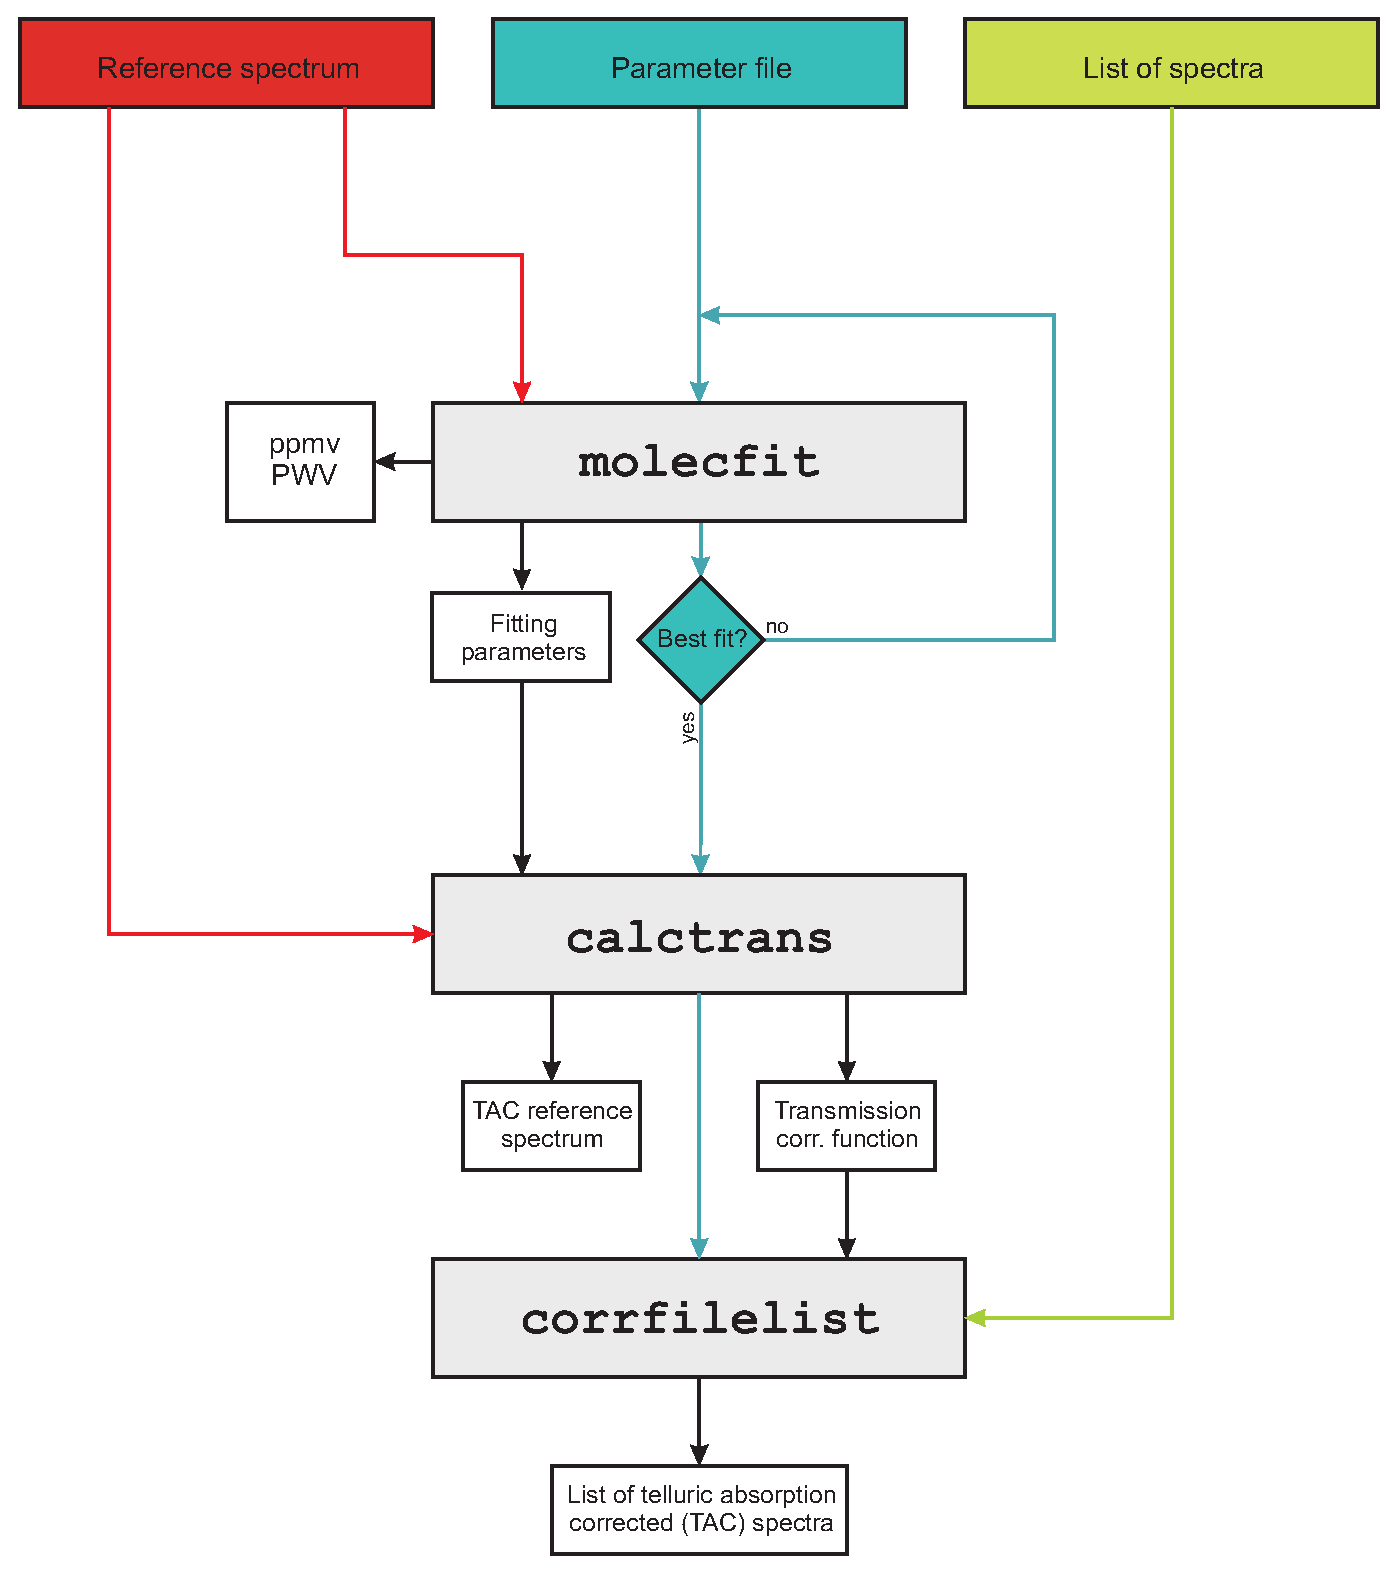
\psfig{file=figures/molecfit_workflow.eps,width=0.9\textwidth}
\caption{Overview of the software workflow. It shows the input and output for
the three executables \mf{}, {\tt calctrans}, and {\tt corrfilelist}
and the connection between these routines.}
\label{fig:mf_overview}
\end{center}
\end{figure}
%-------------------------------------------------------------------------------
%-------------------------------------------------------------------------------
\begin{figure}[ht]
\begin{center}
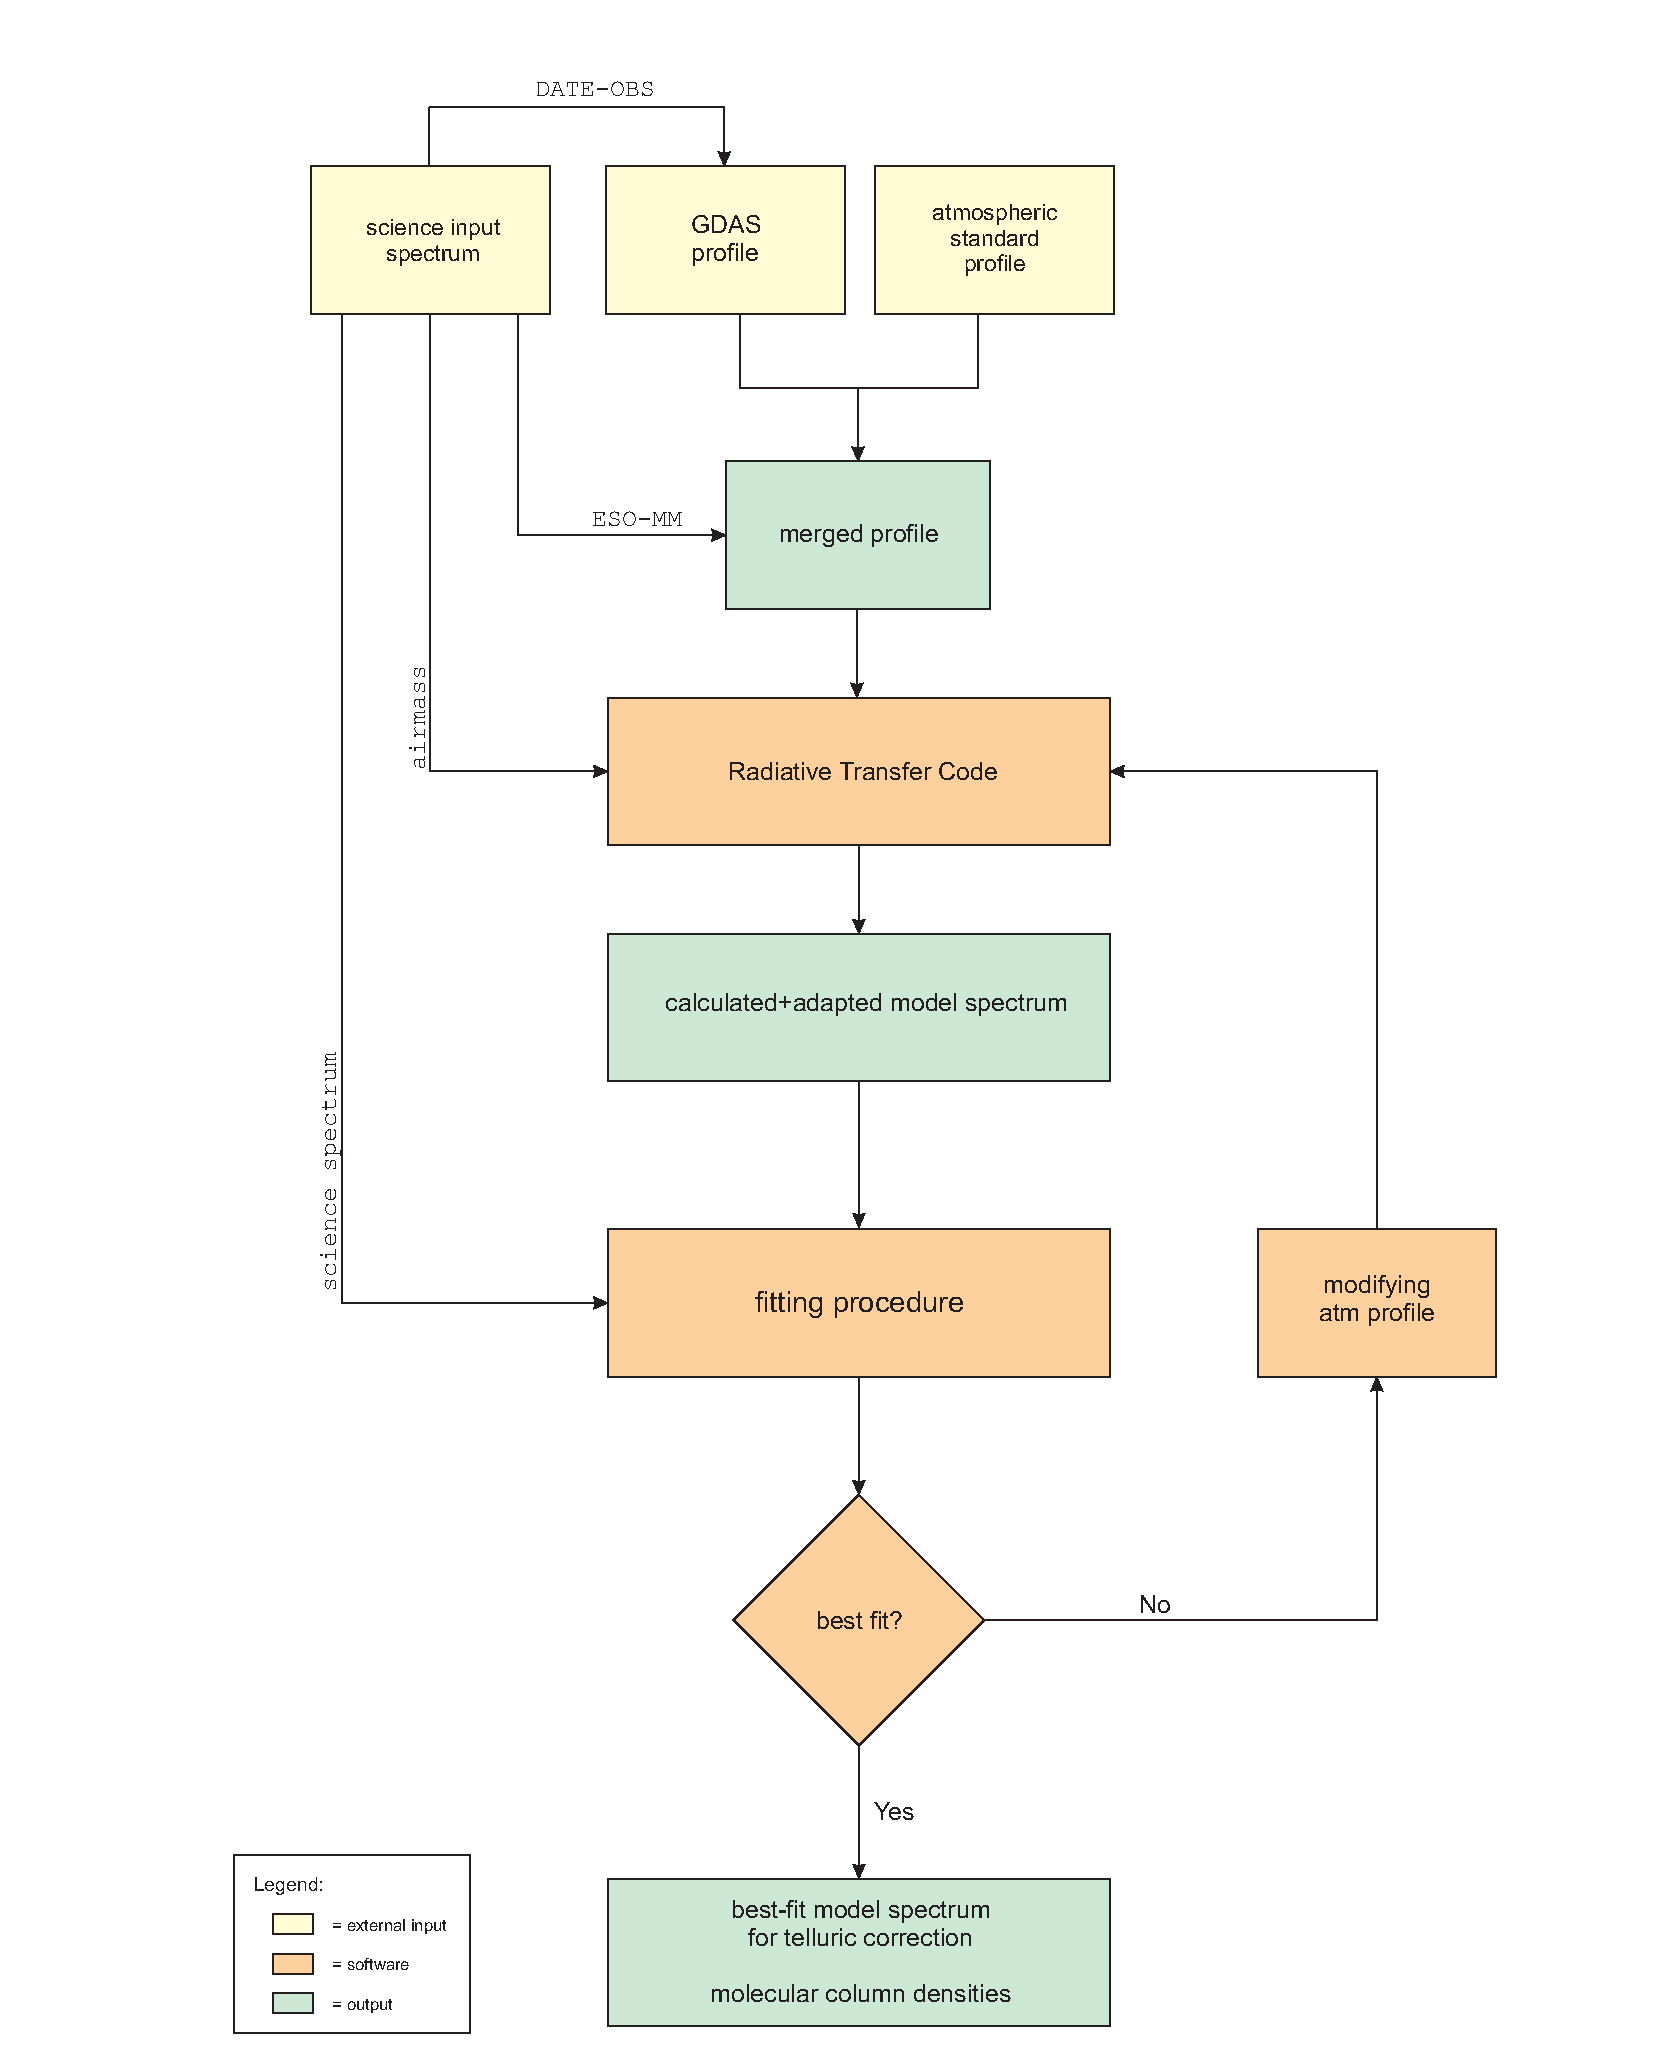
\psfig{file=figures/Overview_SM-03_molecfit.eps,width=0.9\textwidth}
\caption{Workflow of the \mf{} routine.}
\label{fig:mf_detworkflow}
\end{center}
\end{figure}
%-------------------------------------------------------------------------------

First, the code reads the science spectrum from an ASCII table, FITS table, or
FITS image. Furthermore, it reads an ASCII driver file with the user input. If
available, ESO keywords including EMM data are directly taken from a FITS
header. A single atmospheric profile is compiled from data from three sources:
a standard atmospheric profile for a given climate zone, an appropriate
\ac{GDAS} model profile for the time of the observation and the telescope site,
and the corresponding ground-based \ac{EMM} measurements (see
Section~\ref{sec:profiles} for more details). Input for the radiative transfer
model is the resulting merged atmospheric profile (with a possible
pre-selection of relevant molecules) and the target airmass at the time of
observation (see Section~\ref{sec:radcodes}). To match the observed spectrum,
the code adapts the atmospheric spectrum (either transmission or radiation; see
Section~\ref{sec:spectra}) further by flux scaling, wavelength grid correction,
and convolution with a suitable instrumental profile (see
Section~\ref{sec:adaption}). For a radiance spectrum, the contribution of
thermal emission from the telescope is also taken into account (see
Section~\ref{sec:greybody}).

The central component of the algorithm is the comparison/fitting of the
calculated and the input science spectrum by means of {\tt mpfit}
\cite{CMPFIT}. The $\chi^2$ minimisation procedure of this routine is based on
the Levenberg-Marquardt technique (see Mor\'e et al. \cite{MOR80}), an
iterative search algorithm characterised by gradient-controlled jumps in
parameter space. Since this technique is prone to finding local minima,
reasonable starting values and constraints for the fit parameters are required.
{\tt mpfit} checks whether the desired fit quality is reached. If this is not
the case, it changes fit parameters in an appropriate way to search for a better
$\chi^2$. Each function call causes a new calculation of the sky model. For a
change of the molecular abundances, the profiles of molecules can be scaled by
simple factors, which represent a subset of the fit parameters provided to
{\tt mpfit}. The other parameters are coefficients of polynomials for continuum
scaling, coefficients of Chebshev polynomials for the correction of the
wavelength solution, the FWHM of boxcar, Gaussian, and Lorentzian kernels
that are used to build a realistic instrumental profile, and the telescope
emissivity if a radiance spectrum is computed. When a satisfactory fit is
reached after several iterations of the $\chi^2$ minimisation procedure, the
code writes the best-fit spectrum, atmospheric profile, and fit parameters to
output files. The best-fit molecular profiles are integrated to get molecular
columns in ppmv. \mf{} also computes the water vapour content of the
atmosphere in mm. The atmospheric abundances are part of a special output
summary file (see Section~\ref{sec:output}).

The fit parameters are defined in the input driver file (see
Section~\ref{sec:paramfile}). Dynamically setting fit flags to include and
exclude parameters from the fitting procedure allows the code to find a
reasonable solution in a relatively fast and robust way. In detail,
\mf{} follows a plan consisting of six steps by default:
\begin{itemize}
    \item Step 1: scaling of the continuum
    \item Step 2: wavelength and resolution fit
    \item Step 3: rescaling of the continuum
    \item Step 4: fitting of the molecules
    \item Step 5: joint continuum, wavelength, and resolution fit
    \item Step 6: fit of all components (molecules, continuum, wavelength, and
                  resolution)
\end{itemize}
As described in Section~\ref{sec:calling}, it is also possible to focus on the
last step only. Moreover, individual parameters can be fixed for the entire
fitting procedure.

For the telluric absorption correction, the executable {\tt calctrans} has to
be used with the same parameter file as for \mf. {\tt calctrans}
calculates the atmospheric transmission for the full wavelength range of the
input spectrum and corrects this spectrum using this function. These
calculations are separated from the fitting procedure, since the run of a
radiative transfer code for a wide wavelength range is very time consuming.
This is particularly critical if the fit is optimised by several code runs with
different input parameters. For this reason, the fitting procedure should be
performed for several well-defined narrow wavelength ranges that can be
provided by a special ASCII or FITS file (see Section~\ref{sec:paramfile}) if
spectra like those from X-Shooter are processed. Too wide fit ranges are also
not recommended due to the probable failure of the polynomial continuum fit.
The narrow wavelength range of CRIRES allows one to fit the full spectrum at
once. {\tt calctrans} writes a FITS table with the model transmission function,
the telluric absorption corrected spectrum, and a quality flag. Moreover, these
results are provided in the same file format as the input frame, \ie\ ASCII
table, FITS table (with multiple extensions for multiple chips), or 1D FITS
image (with possible extensions for error and quality). For the latter case,
two FITS images are written: one for the correction function and one for the
corrected spectrum (see Section~\ref{sec:output}).

Alternatively, two seperate executables {\tt calctrans\_lblrtm} and 
{\tt calctrans\_convolution} can be used to calculate the atmospheric
transmission and convolve the spectrum respectively.

If other spectra as the fitted one shall be corrected by the same correction
function, an ASCII list of file names can be provided by the input parameter
file (see Section~\ref{sec:paramfile}). The executable {\tt corrfilelist} then
corrects the listed spectra for telluric absorption and saves these spectra in
the same file format as the input files. In addition to the allowed file
formats for \mf, 2D FITS images can be corrected in this way.

\cleardoublepage
%-------------------------------------------------------------------------------
\section{Installation procedure}\label{sec:installation}
%-------------------------------------------------------------------------------
%-------------------------------------------------------------------------------
\subsection{Requirements}\label{sec:requirements}
%-------------------------------------------------------------------------------
The installation of the basic \mf{} binary package requires:
\begin{itemize}
  \item
    C99 compatible compiler (e.g. gcc or clang)
  \item
    glibc 2.11 or newer on Linux or OS X 10.7 or newer
  \item
    common unix utilities (bash, tar, sed, grep, \ldots{})
\end{itemize}

The optional \ac{GUI} to \mf{} requires:

\begin{itemize}
  \item
    Python v2.6 or v2.7 (but not Python v3.x)
  \item
    wxPython v2.8 or newer
  \item
    Python matplotlib v1.0 or newer
  \item
    PyFITS v2.4 or newer
\end{itemize}

The command line client also has optional display features which
require:

\begin{itemize}
  \item gnuplot v4.2 patchlevel 3 or newer
\end{itemize}

%-------------------------------------------------------------------------------
\subsection{Binary installation}
\label{sec:installscript}
%-------------------------------------------------------------------------------

First the downloaded installer needs to be made executable. To do this change
into the directory the installer was downloaded to and run following command
(replacing molecfit\_installer.run with the actual downloaded filename):

\begin{verbatim}
chmod u+x ./molecfit_installer.run
\end{verbatim}

Now the installer can be executed from the same folder with:

\begin{verbatim}
./molecfit_installer.run
\end{verbatim}

It will ask for an installation directory where it will extract its
contents to. It is recommended to choose an empty directory to avoid
overwriting existing files.

After the installer has successfully finished, the \mf{} executables
are installed into the \texttt{bin} subdirectory of the chosen installation
folder. They can be executed by specifying the full or relative path.
Also installed are a set of example parameter files for several
instruments in the \texttt{examples/config} directory. To run a CRIRES example
type:

\begin{verbatim}
<INST_DIR>/bin/molecfit <INST_DIR>/examples/config/molecfit_crires.par
\end{verbatim}

For more details see Section~\ref{sec:running}.

For the \ac{GUI} use the \texttt{molecfit\_gui} executable instead of
\texttt{molecfit}.
For more details on the \ac{GUI} see \cite{MFGUI}.

%-------------------------------------------------------------------------------
\subsection{\ac{GUI} dependencies}
\label{sec:guidependencies}
%-------------------------------------------------------------------------------

The \ac{GUI} requires some additional dependencies to be installed on the system.
To check if the python installation is able to run the \ac{GUI}, following
commands can be run:

\begin{verbatim}
python -c 'import wx'

python -c 'import matplotlib; import matplotlib.backends.backend_wxagg'

python -c 'import pyfits'
\end{verbatim}

If these commands fail please see following site for instructions on how
to install these packages:

\texttt{http://www.eso.org/pipelines/reflex\_workflows/}

%-------------------------------------------------------------------------------
\subsection{Package contents}
\label{sec:pkgcontents}
%-------------------------------------------------------------------------------

The installation package is a self extracting tarball containing the
\mf{} source code and pre-built versions of its third party
dependencies:

\begin{itemize}
  \item
    Common Pipeline Library v6.4.2 and its dependencies cfitsio v3.350,
    wcslib v4.16 and fftw3 v3.3.3 \cite{CPL}
  \item
    Gridded Binary (GRIB) \gribv{} \cite{WGRIB}
  \item
    radiative transfer code \lnflv{} and \lblrtmv{} \cite{LBLRTM}
  \item
    \aerv{} \cite{AER}
\end{itemize}


%-------------------------------------------------------------------------------
\subsection{Source Installation}
\label{sec:sourceinstall}
%-------------------------------------------------------------------------------

Advanced users may want to install everything from source, the basic
instructions for this are outlined here. The installation from source
additionally requires the gfortran compiler.

\subsubsection{CPL compilation}

The CPL sources can be obtained from \cite{CPL}

For \mf{} CPL only requires cfitsio. It can be installed as follows:

\begin{verbatim}
./configure --prefix=/install-location

make

make shared

make install
\end{verbatim}

Then CPL can be install with:

\begin{verbatim}
./configure --prefix=/install-location --with-cfitsio=/install-location

make

make install
\end{verbatim}

See the respective packages documentation for details on the
installation procedure.

\subsubsection{Non-ESO sources compilation}

The rest of the required sources can be downloaded from the same place
the \mf{} binaries installers are available from. The third party
source tarball contains a convenience Makefile to build and install all
packages at once. It can be run with:

\begin{verbatim}
make -f BuildThirdParty.mk install prefix=/install-location
\end{verbatim}

For installation on Mac OS please read the comments in this Makefile.

\subsubsection{Molecfit compilation}

After all dependencies have been installed \mf{} can be compiled from
source into the same location.

This is the only step required if one wants to update \mf{} from
source after previously installing the third party dependencies with the
binary installer.

\begin{verbatim}
./configure --prefix=/install-location --with-cpl=/install-location

make

make install
\end{verbatim}

In order to use \mf{} from this location the environment variable
{\tt LD\_LIBRARY\_PATH} \\(or {\tt DYLD\_LIBRARY\_PATH} on Mac OS) need to be
set. With the bash shell this is done with following command:

\begin{verbatim}
export LD_LIBRARY_PATH=/install-location/lib
\end{verbatim}

Now \mf{} is ready to be used from {\tt /install-location/bin}.

\cleardoublepage
%-------------------------------------------------------------------------------
\section{Running procedure}\label{sec:running}
%-------------------------------------------------------------------------------
%-------------------------------------------------------------------------------
\subsection{Environment variables {\tt molecfit}}\label{sec:variables}
%-------------------------------------------------------------------------------
Before the execution you can to define some environment variables in order to 
change the behavior of molecfit.
\begin{itemize}
  \item TMPDIR: Define the folder where create the temporary directory.
        If it is not define, molecfit use the default 'tmp' directory in the system
  \item MOLECFITDIR: Define the installation directory.
        If it is not define, molecfit use the path of the installation directory provide in compilation time.
  \item MOLECFITDIR\_DATA: Define the data directory.
        If it is not define, molecfit use the path of the data directory create in the installation.
\end{itemize}
Example of use:
\begin{verbatim}
    export TMPDIR=$PWD
    export MOLECFITDIR=$PWD/dest
    export MOLECFITDIR_DATA=$MOLECFITDIR/share/molecfit/data
\end{verbatim}

%-------------------------------------------------------------------------------
\subsection{Calling {\tt molecfit}}\label{sec:calling}
%-------------------------------------------------------------------------------
After the compilation, the executable {\tt molecfit} for the fitting of
molecular transmission and emission is located in the {\tt bin/} directory. It
can be invoked via
% \begin{verbatim}
%     cd <basedir>
%     ./bin/molecfit <parameter file> <optional mode>
% \end{verbatim}
% or
\begin{verbatim}
    cd <arbitrary_dir>
    <fullpath>/bin/molecfit <parameter file> <optional mode>
\end{verbatim}
where {\tt <parameter file>} represents a user-defined parameter file
(including paths). The {\tt <optional mode>} parameter enables the user to run
different modes of the fitting procedure:
\begin{itemize}
    \item `m' - multiple: Choosing this option, the fitting procedure follows
          all five steps described in Section~\ref{sec:algorithm}.
    \item `s' - single run: Only step \#5 is carried out (see
          Section~\ref{sec:algorithm}).
\end{itemize}
Note that in both modes fitting steps that were designated to be skipped (by
setting fit flag $= 0$ in the parameter file) are excluded (see
Section~\ref{sec:paramfile}).

The {\tt <INST\_DIR>/examples} directory contains several examples,
including input spectra (in subfolder {\tt input}) and configuration parameter
files (in subfolder {\tt config}) for the CRIRES, VISIR and X-Shooter
instruments. The CRIRES spectrum represents the best data set for analysing
molecular abundances and is optimally fitted using the parameter file listed
in Section~\ref{sec:paramfile}:
% \begin{verbatim}
%     cd <basedir>
%     ./bin/molecfit examples/config/molecfit_crires.par
% \end{verbatim}
\begin{verbatim}
    cd <arbitrary_dir>
    <fullpath>/bin/molecfit examples/config/molecfit_crires.par
\end{verbatim}
The other examples can be started synonymously.

The conversion of the input data file into a FITS table that is suitable
for the fitting procedure can also be performed by means of the executable
{\tt preptable} plus {\tt <parameter file>} as input parameter. The procedure
is the same as for {\tt molecfit}, but it stops before the fitting is started.

%-------------------------------------------------------------------------------
\subsection{Calling {\tt calctrans}}\label{sec:callingct}
%-------------------------------------------------------------------------------
After the compilation, the executable {\tt calctrans} for the derivation of
the telluric absorption spectrum over the whole spectrum is also located in the {\tt bin/}
directory. It can be run by
% \begin{verbatim}
%     cd <basedir>
%     ./bin/calctrans <parameter file>
% \end{verbatim}
% or
\begin{verbatim}
    cd <arbitrary_dir>
    <fullpath>/bin/calctrans <parameter file>
\end{verbatim}
where {\tt <parameter file>} represents the same user-defined parameter file
(including paths) as used for {\tt molecfit}.

The  telluric  absorption  correction  can be  calculated  for  a  new
spectrum with a different aimass (cf.  Section~\ref{sec:callingct}) by
changing the argument of {\sc  filename} in the {\tt <parameter file>}
(see Section~\ref{sec:params}). If it is an ASCII file, the argument 
of {\sc telalt} must be also changed.

Note  that the  line  kernel  and the  wavelength  correction are  not
modified  by this  approach.  This  requires a  direct  fit with  {\tt
  molecfit}.


%-------------------------------------------------------------------------------
\subsection{Calling {\tt corrfilelist}}\label{sec:callingcfl}
%-------------------------------------------------------------------------------
The {\tt bin/} directory contains the executable {\tt corrfilelist}
for the telluric absorption correction for each of the spectra listed in
an ASCII file given as argument to the {\sc listname} keyword 
in the parameter file. Since the
correction function is not recalculated, airmass differences are not
considered (cf. Section~\ref{sec:callingct}). In the same way as
{\tt calctrans}, {\tt corrfilelist} can be invoked by
% \begin{verbatim}
%     cd <basedir>
%     ./bin/corrfilelist <parameter file>
% \end{verbatim}
% or
\begin{verbatim}
    cd <arbitrary_dir>
    <fullpath>/bin/corrfilelist <parameter file>
\end{verbatim}
where {\tt <parameter file>} represents the same user-defined parameter file
(including paths) as used for {\tt molecfit}.

%-------------------------------------------------------------------------------
\subsection{Calling {\tt calctrans\_lblrtm} and {\tt calctrans\_convolution}}\label{sec:callingct2}
%-------------------------------------------------------------------------------

Alternatively, correction of spectra affected by different (but known)
kernels or different airmasses can  be dealt with in  the following way by  calling two other
executables:
\begin{verbatim}
   cd <arbitrary_dir>
\end{verbatim}
\begin{itemize}
\item 
\begin{verbatim}
<fullpath>/bin/calctrans_lblrtm  <parameter file>
\end{verbatim}
  calculates  the transmission  spectrum from LBLRTM
  using the best fit parameter over the whole wavelength range, with a
  sampling 5 times better than the input spectrum;
\item 
\begin{verbatim}
<fullpath>/bin/calctrans_convolution  <parameter file>
\end{verbatim}
performs the  convolution of  the
  spectrum produced by  {\tt calctrans\_lblrtm} with  the user-provided kernel.
\end{itemize}

A typical use is the following:
\begin{enumerate}
\item the user knows well the  kernel for the spectra provided by each
  fiber of  a multi-fiber spectrograph.   {\tt Molecfit} is  called to
  fit the  molecular content  on an input  spectrum (argument  of {\sc
    filename})  corresponding to  a  given fiber;  the parameter  file
  includes  the filename  with the  corresponding kernel  (argument of
  {\sc kernel\_file});
\item once a satisfactory fit is obtained, {\tt calctrans\_lblrtm} is
  run with the parameter file unchanged;
\item then {\tt calctrans\_convolution} is called with the same
  parameter file in which the name of the input file (argument of
  {\sc filename}) has been changed for the spectrum of another fiber, and
  where the kernel filename (argument of {\sc kernel\_file}) has been changed
  to provide the corresponding kernel. This step can be repeated for each
  spectra.
\end{enumerate}
On  the  other  hand,  if   the  airmass  for  another  fiber  differs
significantly from the first, {\tt calctrans\_lblrtm} should be called
with  the  same parameter  file  where  the  name  of the  input  file
(argument of {\sc  filename}) has been changed to the  filename of the
corresponding  spectrum.  The  telescope altitude  (argument  of  {\sc
  telalt}) must be changed also if the input file is an ASCII file.



%-------------------------------------------------------------------------------
\subsection{The parameter file}\label{sec:paramfile}
%-------------------------------------------------------------------------------
All parameters needed for the fit are read from an ASCII parameter file, which
contains parameter names, descriptions, and initial values. Example files can
be found in the folder {\tt examples/config/}.

The file is divided into sections, where parameters belonging together are
grouped. These sections incorporate the directory structure (labelled
{\tt DIRECTORY STRUCTURE}), the required input ({\tt INPUT DATA}), output
options ({\tt RESULTS}), the precision of the fit ({\tt FIT PRECISION}),
molecular information ({\tt MOLECULAR COLUMNS}), the fit of the background and
the continuum ({\tt BACKGROUND AND CONTINUUM}), the wavelength fit
({\tt WAVE\-LENGTH SOLUTION}), the resolution fit ({\tt RESOLUTION}),
environmental parameters ({\tt AMBIENT}\linebreak {\tt PARAMETERS}), and the
atmospheric profiles ({\tt ATMO\-SPHERIC PROFILES}). The individual parameters
are given one per line. The parameter name plus a trailing colon and space is
followed by one or more parameter values, which also have to be separated by
spaces. Lines beginning with a hash key are assumed to be comments and are
skipped. Thus, next to removing parameter lines, there are several options to
``deactivate'' a parameter in the parameter file:

Command ``active'':
\begin{verbatim}
ftol: 1e-2
\end{verbatim}

Command ``deactivated'' (commented out):
\begin{verbatim}
#ftol: 1e-2
\end{verbatim}

Command ``deactivated'' (no trailing colon):
\begin{verbatim}
ftol 1e-2
\end{verbatim}

Command ``deactivated'' (no parameter value)
\begin{verbatim}
ftol:
\end{verbatim}
or
\begin{verbatim}
ftol
\end{verbatim}

In the following, {\tt examples/config/molecfit\_crires.par} is shown as
an example of a parameter file. Individual parameters are explained in
Section~\ref{sec:params}:

{\small
\begin{verbatim}
### Driver for MOLECFIT

## INPUT DATA

# Data file name (path relative to the current directory or absolute path)
filename: examples/input/crires_spec_jitter_extracted_0000.fits

# ASCII list of files to be corrected for telluric absorption using the
# transmission curve derived from the input reference file (path of list and
# listed files relative to the current directory or absolute path; default: "none")
listname: none

# Type of input spectrum -- 1 = transmission (default); 0 = emission
trans: 1

# Names of the file columns (table) or extensions (image) containing:
# Wavelength  Flux  Flux_Err  Mask
# - Flux_Err and/or Mask can be avoided by writing 'NULL'
# - 'NULL' is required for Wavelength if it is given by header keywords
# - parameter list: col_lam, col_flux, col_dflux, and col_mask
columns: Wavelength Extracted_OPT Error_OPT NULL

# Default error relative to mean for the case that the error column is missing
default_error: 0.01

# Multiplicative factor to convert wavelength to micron
# (e.g. nm -> wlgtomicron = 1e-3)
wlgtomicron: 1e-3

# Wavelengths in vacuum (= vac) or air (= air)
vac_air: vac

# ASCII or FITS table for wavelength ranges in micron to be fitted
# (path relative to the current directory or absolute path; default: "none")
wrange_include: none

# ASCII or FITS table for wavelength ranges in micron to be excluded from the
# fit (path relative to the current directory or absolute path; default: "none")
wrange_exclude: none

# ASCII or FITS table for pixel ranges to be excluded from the fit
# (path relative to the current directory or absolute path; default: "none")
prange_exclude: examples/config/exclude_crires.dat

## RESULTS

# Directory for output files (path relative to the current directory or absolute path)
output_dir: output

# Name for output files
# (supplemented by "_fit" or "_tac" as well as ".asc", ".atm", ".fits",
# ".par, ".ps", and ".res")
output_name: molecfit_crires

# Plot creation: gnuplot is used to create control plots
# W - screen output only (incorporating wxt terminal in gnuplot)
# X - screen output only (incorporating x11 terminal in gnuplot)
# P - postscript file labelled '<output_name>.ps', stored in <output_dir>
# combinations possible, i.e. WP, WX, XP, WXP (however, keep the order!)
# all other input: no plot creation is performed
plot_creation: XP

# Create plots for individual fit ranges? -- 1 = yes; 0 = no
plot_range: 0

## FIT PRECISION

# Relative chi2 convergence criterion
ftol: 1e-2

# Relative parameter convergence criterion
xtol: 1e-2

## MOLECULAR COLUMNS

# List of molecules to be included in the model
# (default: 'H2O', N_val: nmolec)
list_molec: H2O CH4 O3

# Fit flags for molecules -- 1 = yes; 0 = no (N_val: nmolec)
fit_molec: 1 1 1

# Values of molecular columns, expressed relatively to the input ATM profile
# columns (N_val: nmolec)
relcol: 1. 1. 1.

## BACKGROUND AND CONTINUUM

# Conversion of fluxes from phot/(s*m2*mum*as2) (emission spectrum only) to
# flux unit of observed spectrum:
# 0: phot/(s*m^2*mum*as^2) [no conversion]
# 1: W/(m^2*mum*as^2)
# 2: erg/(s*cm^2*A*as^2)
# 3: mJy/as^2
# For other units, the conversion factor has to be considered as constant term
# of the continuum fit.
flux_unit: 0

# Fit of telescope background -- 1 = yes; 0 = no (emission spectrum only)
fit_back: 0

# Initial value for telescope background fit (range: [0,1])
telback: 0.1

# Polynomial fit of continuum --> degree: cont_n
fit_cont: 1

# Degree of coefficients for continuum fit
cont_n: 3

# Initial constant term for continuum fit (valid for all fit ranges)
# (emission spectrum: about 1 for correct flux_unit)
cont_const: 1.

## WAVELENGTH SOLUTION

# Refinement of wavelength solution using a polynomial of degree wlc_n
fit_wlc: 1

# Polynomial degree of the refined wavelength solution
wlc_n: 3

# Initial constant term for wavelength correction (shift relative to half
# wavelength range)
wlc_const: 0.

## RESOLUTION

# Fit resolution by boxcar -- 1 = yes; 0 = no
fit_res_box: 0

# Initial value for FWHM of boxcar relative to slit width (>= 0. and <= 2.)
relres_box: 0.

# Voigt profile approximation instead of independent Gaussian and Lorentzian
# kernels? -- 1 = yes; 0 = no
kernmode: 0

# Fit resolution by Gaussian -- 1 = yes; 0 = no
fit_res_gauss: 1

# Initial value for FWHM of Gaussian in pixels
res_gauss: 1.

# Fit resolution by Lorentzian -- 1 = yes; 0 = no
fit_res_lorentz: 0

# Initial value for FWHM of Lorentzian in pixels
res_lorentz: 0.5

# Size of Gaussian/Lorentzian/Voigtian kernel in FWHM
kernfac: 300.

# Variable kernel (linear increase with wavelength)? -- 1 = yes; 0 = no
varkern: 0

# ASCII file for kernel elements (one per line; normalisation not required)
# instead of synthetic kernel consisting of boxcar, Gaussian, and Lorentzian
# components (path relative to the current directory or absolute path; default: "none")
kernel_file: none

## AMBIENT PARAMETERS

# If the input data file contains a suitable FITS header, the keyword names of
# the following parameters will be read, but the corresponding values will not
# be used. The reading of parameter values from this file can be forced by
# setting keywords to NONE.

# Observing date in years or MJD in days
obsdate
obsdate_key: MJD-OBS

# UTC in s
utc
utc_key: UTC

# Telescope altitude angle in deg
telalt
telalt_key: ESO TEL ALT

# Humidity in %
rhum
rhum_key: ESO TEL AMBI RHUM

# Pressure in hPa
pres
pres_key: ESO TEL AMBI PRES START

# Ambient temperature in deg C
temp
temp_key: ESO TEL AMBI TEMP

# Mirror temperature in deg C
m1temp
m1temp_key: ESO TEL TH M1 TEMP

# Elevation above sea level in m (default is Paranal: 2635m)
geoelev
geoelev_key: ESO TEL GEOELEV

# Longitude (default is Paranal: -70.4051)
longitude
longitude_key: ESO TEL GEOLON

# Latitude (default is Paranal: -24.6276)
latitude
latitude_key: ESO TEL GEOLAT

## INSTRUMENTAL PARAMETERS

# Slit width in arcsec (taken from FITS header if present)
slitw: 0.4
slitw_key: ESO INS SLIT1 WID

# Pixel scale in arcsec (taken from this file only)
pixsc: 0.086
pixsc_key: NONE

## ATMOSPHERIC PROFILES

# Reference atmospheric profile
ref_atm: equ.atm

# Specific GDAS-like input profile (P[hPa] HGT[m] T[K] RELHUM[%]) (path
# relative to the installation directory or absolute path). In the case of "none", no GDAS
# profiles will be considered. The default "auto" performs an automatic
# retrieval.
gdas_prof: auto

# Grid of layer heights for merging ref_atm and GDAS profile. Fixed grid = 1
# (default) and natural grid = 0.
layers: 1

# Upper mixing height in km (default: 5) for considering data of a local meteo
# station. If emix is below geoelev, rhum, pres, and temp are not used for
# modifying the corresponding profiles.
emix: 5

# PWV value in mm for the input water vapour profile. The merged profile
# composed of ref_atm, GDAS, and local meteo data will be scaled to this value
# if pwv > 0 (default: -1 -> no scaling).
pwv: -1

end
\end{verbatim}
}

%\pagebreak

%-------------------------------------------------------------------------------
\subsection{The parameters}\label{sec:params}
%-------------------------------------------------------------------------------
In the following, the individual parameters are explained in more detail by
following the order as they appear in the parameter file.

% {\bf\large\tt\#\# DIRECTORY STRUCTURE:}
% \begin{itemize}
% \item {\sc basedir}: Base directory (default: ".") for the following folder
% structure:
% \begin{verbatim}
%                |--bin/
%                |
%                |--config/
%   <basedir>----|
%                |--data/
%                |
%                |--output/
% \end{verbatim}
% A relative or an absolute path can be provided. In the former case, \mf\
% has to be started in <basedir>. The subfolder ``bin/'' of <basedir> is to
% contain all required executables (see Section~\ref{sec:installation}).
% Configuration files for the radiative transfer codes and mandatory input data
% (line parameter database, atmospheric profiles, or molecular cross section
% files) have to be located in ``config/'' and ``data/'', respectively. Finally,
% ``output/'' is the default folder for all resulting files described in
% Section~\ref{sec:output}. The output directory can be modified by the parameter
% {\sc output\_dir} (see below). For example \mf\ parameter files and input
% spectra, we have created the directory ``examples/'' with the subfolders
% ``config/'' and ``input/''. The names of these folders are arbitrary and their
% presence is not expected by the code.
% \end{itemize}

{\bf\large\tt\#\# INPUT DATA:}
\begin{itemize}
\item {\sc filename}: Path and name of the input spectrum. The path has to be
relative to the current directory or absolute. The accepted file formats for the
input spectrum are ASCII and FITS. The spectral data of the latter has to be
provided either in table form (multiple FITS extensions for different chips) or
as 1D image (with optional error and quality data in additional FITS
extensions).  See section \ref{sec:inputspec} for more information about the
input file format.
\item {\sc listname}: Input ASCII list of files for {\tt corrfilelist}, which
corrects spectra for telluric absorption using the transmission curve derived
by {\tt calctrans}. The path to the list and the listed files has to be
relative to the current directory or absolute. In contrast to {\sc filename}, the
listed files can also be 2D FITS images. By default, no file list is expected
(``none'').
\item {\sc trans}: type of input spectrum (1 = transmission, 0 = emission;
default = 1).
\item {\sc columns}: Column names of the input file containing information on
wavelength, flux, flux\_err, and mask. The latter two are optional and can be
disabled by setting them to ``NULL''. For ASCII files, the column names are
irrelevant, with the exception of ``NULL'' input. In the case of FITS images,
the given labels are compared to the FITS extension names (keyword
``EXTNAME''). Since it is expected that the flux data is in the first layer of
the FITS file (0th extension), the existence of a corresponding FITS keyword is
not required for this column. Internally, the code denotes the columns as
{\sc col\_lam}, {\sc col\_flux}, {\sc col\_dflux}, and {\sc col\_mask}.
\item {\sc default\_error}: Default error relative to the mean in case
the error column is missing (column name = ``NULL'', see previous
record).
\item {\sc wlgtomicron}: Multiplicative factor to convert input wavelength unit
into $\mu$m. For example, for nm this parameter has to set to $10^{-3}$.
\item {\sc vac\_air}: Wavelengths in vacuum (= ``vac'') or air (= ``air'')?
This parameter depends on the instrument and the wavelength calibration
approach.
\item {\sc wrange\_include}: ASCII or FITS table for wavelength ranges to be
fitted. The path to the file has to be relative to the current directory or absolute.
Except for empty lines and comment lines starting with \#, each line of an
ASCII file has to provide a lower and an upper wavelength limit in $\mu$m. FITS
tables must contain exactly two columns. The column labels are not fixed. If a
range table is not desired and the full spectrum shall be fitted, ``none'' can
be given. This is also the default value.
\item {\sc wrange\_exclude}: ASCII or FITS table for wavelength ranges to be
excluded from the fit. The path to the file has to be relative to the current directory
or absolute. Except for empty lines and comment lines starting with \#, each
line of an ASCII file has to provide a lower and an upper wavelength limit in
$\mu$m. FITS tables must contain exactly two columns. The column labels are not
fixed. If the exclusion of wavelength ranges is not desired, ``none'' can be
given. This is also the default value.
\item {\sc prange\_exclude}: ASCII or FITS table for pixel ranges to be
excluded from the fit. The path to the file has to be relative to the current directory
or absolute. Except for empty lines and comment lines starting with \#, each
line of an ASCII file has to provide a lower and an upper pixel. FITS tables
must contain exactly two columns. The column labels are not fixed. The pixel
counting starts with 1. If there are several chips, the pixel counting
continues at chip limits. If a range table is not desired and all pixels shall
be fitted, ``none'' can be given. This is also the default value.
\end{itemize}

{\bf\large\tt\#\# RESULTS:}
\begin{itemize}
\item {\sc output\_dir}: Output directory as path relative to the current directory or
absolute path (see also Section {\tt DIRECTORY STRUCTURE)}. The folder is
created if it does not exist.
\item {\sc output\_name}: Unique name space for output files. The extensions
are supplemented by ``\_fit'' or ``\_tac'' as well as ``.asc'', ``.atm'',
``.fits'', ``.par'', ``.ps'', and ``.res''. See Section~\ref{sec:output} for
more details.
\item {\sc plot\_creation}: {\tt molecfit} invokes {\tt gnuplot} to create
control plots for verifying the fit. For each fit range, an individual plot
is created, which contains a comparison of the observed and the modelled
spectrum and their residual. An overview plot for the entire wavelength range
is also produced. Finally, {\tt calctrans} creates a plot that shows the
initial and the telluric absorption corrected spectrum. This parameter allows
specifying the output terminal of gnuplot:
W - screen output incorporating wxt terminal,
X - screen output incorporating x11 terminal,
P - postscript files labelled `<output\_name>\_fit.ps',
    `<output\_name>\_fit\_<fitrange>.ps', and `<output\_name>\_tac.ps' (stored
    in <output\_dir>).
Also, arbitrary combinations are possible, \eg\ WP for wxt terminal and
postscript, or WX for wxt and x11 terminal output.
\item {\sc plot\_range}: Flag for creation of plots of individual fit ranges
(1 = yes, 0 = no). If the flag is set to 0, the files labelled
`<output\_name>\_fit\_<fitrange>.ps' are not produced.
\end{itemize}

{\bf\large\tt\#\# FIT PRECISION:}
\begin{itemize}
\item {\sc ftol}: relative $\chi^2$ convergence criterion.
\item {\sc xtol}: relative parameter convergence criterion.
\end{itemize}

{\bf\large\tt\#\# MOLECULAR COLUMNS:}
\begin{itemize}
\item {\sc list\_molec}: List of molecules separated by blanks, which are
included in the model. Note that only those molecules are valid, which are
also present in the standard atmospheric profile {\sc ref\_atm} (see also
Section~\ref{sec:mipas}).
\item {\sc fit\_molec}: Fit flags (1 = yes, 0 = no) separated by blanks for
list of molecules. \# has to match number of molecules in {\sc list\_molec}.
Example: {\sc 1 0 1} implies that only the first and third molecule are
fitted. The middle molecule is included statically in the fit, \ie\ its
abundance is not varied in the fit.
\item {\sc relcol}: Relative molecular column densities separated by blanks,
normalised to the values in the input atmospheric profile (1 = 100\%). \# has
to match number of molecules in {\sc list\_molec}.
\end{itemize}

{\bf\large\tt\#\# BACKGROUND AND CONTINUUM:}
\begin{itemize}
\item {\sc flux\_unit}: Conversion of fluxes from phot/(s$\cdot$m$^2\cdot$
$\mu$m$\cdot$arcsec$^2$) (emission spectrum only) to flux unit of observed
spectrum: 0 = phot/(s$\cdot$m$^2\cdot$$\mu$m$\cdot$arcsec$^2$) (--> no
conversion), 1 = W/(m$^2\cdot$$\mu$m$\cdot$arcsec$^2$),
2 = erg/(s$\cdot$cm$^2\cdot$\AA$\cdot$arcsec$^2$), 3 = mJy/arcsec$^2$.
For other units differing from the offered units by a constant factor, the
constant term of the continuum fit parameters {\sc cont\_const} has to be
multiplied by the conversion factor. For non-flux-calibrated spectra provided
in analogue-to-digital units (ADU), the default 0 is the best choice.
\item {\sc fit\_back}: fit of telescope background (1 = yes, 0 = no); used for
emission spectrum fit only.
\item {\sc telback}: initial emissivity value for telescope background grey
body fit; used for emission spectrum fit only.
\item {\sc fit\_cont}: Flag for polynomial fit of the continuum (1 = yes,
0 = no). For each fit range/chip, the model spectrum is multiplied by the
resulting polynomial.
\item {\sc cont\_n}: degree of polynomial for the continuum fit.
\item {\sc cont\_const}: Initial constant term of the polynomial for the
continuum fit. The same value is used for all fit ranges/chips. By default,
1 is assumed. Since all higher terms are set to 0 at the beginning, the fitting
procedure starts without a continuum correction if the default setting is used.
For sky emission spectra with correct {\sc flux\_unit}, the true continuum
correction factor should be very close to the default value 1.
\end{itemize}

{\bf\large\tt\#\# WAVELENGTH SOLUTION:}
\begin{itemize}
\item {\sc fit\_wlc}: flag for refinement of wavelength solution (1 = yes,
0 = no).
\item {\sc wlc\_n}: degree of Chebyshev polynomial for refined wavelength
solution.
\item {\sc wlc\_const}: Constant term of the Chebyshev polynomial for the
wavelength solution, which is derived for each chip independently. The provided
constant term is used for all chips. The given value represents a shift
relative to half the wavelength range of the input spectrum. By default,
0 is assumed. Since the linear term and the higher terms are set to 1 and 0,
respectively, at the beginning, the fitting procedure starts without a
wavelength correction if the default setting is used.
\end{itemize}

{\bf\large\tt\#\# RESOLUTION:}\\[0.5cm]
The resolution fit incorporates a combined, boxcar, Gaussian, and
Lorentzian convolution. The latter two convolutions result in a Voigt profile.
\begin{itemize}
\item {\sc fit\_res\_box}: flag for resolution fit using a boxcar filter
(1 = yes, 0 = no).
\item {\sc relres\_box}: Initial value for FWHM of boxcar relative to slit
width ($\geq 0$ and $\leq 2$). A value of 0 combined with
{\sc fit\_res\_box}~=~0 switches off the convolution of a boxcar.
\item {\sc kernmode}: By default (= 0), spectra are convolved by independent
Gaussian and Lorentzian kernels. It is also possible to perform only one
convolution with a kernel derived from a Voigt profile approximation (= 1),
which also uses the FWHM of Gaussian and Lorentzian as input.
\item {\sc fit\_res\_gauss}: flag for resolution fit using a Gaussian filter
(1 = yes, 0 = no).
\item {\sc res\_gauss}: Initial value for FWHM of Gaussian (in pixels). A value
of 0 combined with \\ {\sc fit\_res\_gauss}~=~0 switches off the convolution of
a Gaussian.
\item {\sc fit\_res\_lorentz}: flag for resolution fit using a Lorentzian
filter (1 = yes, 0 = no).
\item {\sc res\_lorentz}: Initial value for FWHM of Lorentzian (in pixels). A
value of 0 combined with \\ {\sc fit\_res\_lorentz}~=~0 switches off the
convolution of a Lorentzian.
\item {\sc kernfac}: Kernel size in units of FWHM. Depending on
{\sc kernmode} either the Gaussian and Lorentzian kernels or the combined
Voigt profile kernel are relevant. By default, a value of 3 is assumed.
\item {\sc varkern}: Flag for selecting a constant (= 0) or a variable kernel
(= 1). In the latter case, all FWHM values are related to the central
wavelength of the full wavelength range. The variable kernel increases linearly
with wavelength, \ie\ the resolution is constant. X-Shooter Echelle spectra
show this behaviour. For spectra where the object profile in the slit mainly
determines the kernel, the default constant kernel option is recommended.
\item {\sc kernel\_file} ASCII file for fixed kernel elements (pixels) instead
of a synthetic kernel consisting of boxcar, Gaussian, and Lorentzian
components. The latter is the default case and requires ``none''. The path to
the file has to be relative to the current directory or absolute. In the file, each
kernel element has to be given on a separate line. It is not required that the
kernel has been normalised to 1. Note that a given {\sc kernel\_file} overrules
all other parameters related to the line profile. The kernel will not be
fitted and will not depend on the wavelength (irrespective of {\sc varkern}).
\end{itemize}

{\bf\large\tt\#\# AMBIENT PARAMETERS:}\\[0.5cm]
The parameters of this section are only required if the input spectrum is
provided as ASCII file or if the ESO FITS header keywords are missing or differ
from the default names. The use of a specific value from the parameter file can
be forced by setting the keyword name to ``NONE''. If no keyword is provided
by the input file (\eg\ ASCII file), it is not required to set the keyword
names to ``NONE''.
\begin{itemize}
\item {\sc obsdate}: Observing date in years, \eg\ 2008.566, or MJD in days.
This parameter is required for the retrieval of GDAS data.
\item {\sc obsdate\_key}: FITS keyword name for {\sc obsdate} (default:
``MJD-OBS'').
\item {\sc utc}: UTC in s, starting at 00:00. This parameter is required for
the retrieval of GDAS data.
\item {\sc utc\_key}: FITS keyword name for {\sc utc} (default: ``UTC'').
\item {\sc telalt}: altitude angle of telescope in deg.
\item {\sc telalt\_key}: FITS keyword name for {\sc telalt} (default:
``ESO TEL ALT'').
\item {\sc rhum}: Relative humidity in \% for {\sc geoelev}. This parameter is
only relevant if {\sc emix} is larger than {\sc geoelev}.
\item {\sc rhum\_key}: FITS keyword name for {\sc rhum} (default:
``ESO TEL AMBI RHUM'').
\item {\sc pres}: Pressure in hPa for {\sc geoelev}. This parameter is only
relevant if {\sc emix} is larger than {\sc geoelev}.
\item {\sc pres\_key}: FITS keyword name for {\sc pres} (default:
``ESO TEL AMBI PRES START'').
\item {\sc temp}: Ambient temperature in $^\circ$C for {\sc geoelev}. This
parameter is only relevant if {\sc emix} is larger than {\sc geoelev}.
\item {\sc temp\_key}: FITS keyword name for {\sc temp} (default:
``ESO TEL AMBI TEMP'').
\item {\sc m1temp}: Temperature of primary mirror M1 in $^\circ$C. This
parameter is only relevant for emission spectra (\ie\ {\sc trans}~=~0), where
the thermal emission of the telescope has to be considered.
\item {\sc m1temp\_key}: FITS keyword name for {\sc m1temp} (default:
``ESO TEL TH M1 TEMP'').
\item {\sc geoelev}: elevation above sea level in m (default is Paranal:
2635\,m).
\item {\sc geoelev\_key}: FITS keyword name for {\sc geoelev} (default:
``ESO TEL GEOELEV'').
\item {\sc longitude}: Longitude in deg (default is Paranal: -70.4051). This
parameter is required for the retrieval of GDAS data.
\item {\sc longitude\_key}: FITS keyword name for {\sc longitude} (default:
``ESO TEL GEOLON'').
\item {\sc latitude}: Latitude in deg (default is Paranal: -24.6276). This
parameter is required for the retrieval of GDAS data.
\item {\sc latitude\_key}: FITS keyword name for {\sc latitude} (default:
``ESO TEL GEOLAT'').

\end{itemize}
{\bf\large\tt\#\# INSTRUMENTAL PARAMETERS:}
\begin{itemize}
\item {\sc slitw}: Slit width in arcsec. The provided value is only taken into
account if the ESO keyword ``ESO INS SLIT1 WID'' does not exist and the
instrument is not X-Shooter (special keyword finding routine). For CRIRES and
VISIR, the stated keyword is usually present.
\item {\sc slitw\_key}: FITS keyword name for {\sc slitw} (default:
``ESO INS SLIT1 WID'').
\item {\sc pixsc}: Pixel scale in arcsec. This parameter has to be provided
manually, since this information could not be found in the ESO file headers of
the investigated instruments.
\item {\sc pixsc\_key}: FITS keyword name for {\sc pixsc}. The default is
``NONE'', \ie\ the parameter is read from the parameter file.
\end{itemize}

{\bf\large\tt\#\# ATMOSPHERIC PROFILES:}
\begin{itemize}
\item {\sc ref\_atm}: Reference atmospheric profile (standard profile). By
default, it is set to ``equ.atm'', which is located in the dedicated folder
``data/profiles/mipas/''. See Section~\ref{sec:mipas} for more information.
\item {\sc gdas\_prof}: Specific GDAS-like input profile (format:
P[hPa] HGT[m] T[K] RELHUM[\%], see Section~\ref{sec:gdas}). The path to the
file has to be relative to the installation directory or absolute. In the case of ``none'',
no GDAS profiles will be considered. The default option ``auto'' causes an
automatic retrieval either from a local library or a web-server (see
Section~\ref{sec:processing}).
\item {\sc layers}: Flag for grid of layer heights required for merging
{\sc ref\_atm} and GDAS profiles. The default option is 1, which selects a
fixed grid with 50 layers for Cerro Paranal (see Section~\ref{sec:processing}).
If the parameter is set to 0, a natural grid is used, \ie\ all layer heights of
{\sc ref\_atm} and the GDAS profile are combined, which tends to significantly
increase the number of layers compared to the default option. If local meteo
data are considered (see {\sc emix}), {\sc geoelev} is also added to the grid.
\item {\sc emix}: Upper mixing height in km for considering data of a local
meteorological station (see Section~\ref{sec:emm}). Above this level, the
influence of the meteo data is expected to be zero (see
Section~\ref{sec:processing}). For Cerro Paranal, the default value of 5\,km
is assumed. If {\sc emix} is below {\sc geoelev}, no local meteo data are
considered, \ie\ the content of {\sc rhum}, {\sc pres}, and {\sc temp} is
not used for modifying the merged profiles.
\item {\sc pwv}: Precipitable water vapour (PWV) value in mm for the input
water vapour profile. The merged profile composed of {\sc ref\_atm}, GDAS, and
local meteo data (see Section~\ref{sec:profiles}) will be scaled to this value
if {\sc pwv} is positive. By default ({\sc pwv}~=~-1), the manipulation of the
input water vapour profile is switched off. The {\sc relcol} value for water
vapour refers to the given {\sc pwv}.
\end{itemize}

The keyword {\sc end} is optional. It marks the last line that is considered by
the file reading routine. Any text beyond {\sc end} is ignored.

%-------------------------------------------------------------------------------
\subsection{Format of the input spectrum}\label{sec:inputspec}
%-------------------------------------------------------------------------------
\subsubsection{Accepted file formats}\label{sec:inputspec_accepted}
%-------------------------------------------------------------------------------
Molecfit currently accepts the following formats:
\begin{enumerate}
    \item ASCII.
    \item FITS binary table,
    \item 1D FITS image,
    \item Multi-dimentional FITS image,
\end{enumerate}
and recognizes it in the following way:
\begin{enumerate}[i]
    \item If the file is not a FITS file, Molecfit assumes an ASCII format.
    \item If the file is a FITS file, Molecfit then looks at the presence of
          extensions.  Molecfit assumes a 1D image format.  (Note that the FITS
          keyword {\sc EXTEND} only indicates that an extension may be present,
          not that it is present!)
    \item If there is at least  one extension, Molecfit uses the keyword
          {\sc XTENSION} in the extension(s) to identify if the file is
          a---possibly multi-extension---FITS binary table
          ({\sc XTENSION=BINTABLE}) or an image ({\sc XTENSION=IMAGE}).  If the
          file is an image, Molecfit then uses the {\sc NAXIS} keyword to
          distinguish between 1D, 2D and 3D images.
\end{enumerate}

%-------------------------------------------------------------------------------
\subsubsection{A note regarding the mask values}\label{sec:inputspec_mask}
%-------------------------------------------------------------------------------
The default behavior of Molecfit is that all values are either 0 or 1. A value
of 0 indicates that the value must not be used by the fit and a value of 1
indicates that the value should be used by the fit. However, Molecfit also
checks that values other than 0 and 1 are used. If this is the case, 0 is
assumed to be ok and all other values cause pixel rejection.

Possible {\sc NAN} in the flux and error columns are substituted by zero flux
and the corresponding pixel is rejected for the fit. The same is performed for
negative errors.


%-------------------------------------------------------------------------------
\subsubsection{Format of the ASCII files}\label{sec:inputspec_ascii}
%-------------------------------------------------------------------------------
Two columns are mandatory: the first column must provide the wavelength and the
second column, the flux. Two additional columns are optional: the 1-\(\sigma\)
error on the flux and the mask.

The 'columns' entry in the parameter file should be a list of 4 names, which are
unimportant, except for {\sc NULL}.  However, it is a good practice---if only
for readability---to use
\begin{verbatim}
	columns: Wavelength Flux Flux_Err Mask
\end{verbatim}

If the error on the flux and/or the mask are not provided, {\sc Flux\_Err}
and/or {\sc Mask} should be replaced by {\sc NULL}.

%-------------------------------------------------------------------------------
\subsubsection{Format of the FITS binary tables}\label{sec:inputspec_bintable}
%-------------------------------------------------------------------------------
Two columns are mandatory: the first column must provide the wavelength and the
second column the flux. Two additional columns are optional: the 1-\(\sigma\)
error on the flux and  the mask.

The 'columns' entry in the parameter file should be:
\begin{verbatim}
	columns: wavelength_label flux_label flux_err_label mask_label
\end{verbatim}
where the field is made of the label (title) of the column in the FITS binary
table. Note that the labels are case-sensitive! If the error on the flux and/or
the mask are not provided, {\sc flux\_err\_label} and/or {\sc mask\_label}
should be replaced by {\sc NULL}.

Example: reduced CRIRES (pre-upgrade) file using the optimally extracted fluxes.
\begin{verbatim}
	columns: Wavelength Extracted_OPT Error_OPT NULL
\end{verbatim}

%-------------------------------------------------------------------------------
\subsubsection{Format of the FITS 1D image data}\label{sec:inputspec_fits1dimg}
%-------------------------------------------------------------------------------
In the case of FITS image data, the wavelength information is provided through
the FITS keywords {\sc CRPIX1}, {\sc CRVAL1} and {\sc CRPIX1} if the wavelength
vector is not provided.

The 'columns' entry in the parameter file should be:
\begin{verbatim}
	columns: NULL Flux NULL NULL
\end{verbatim}

%-------------------------------------------------------------------------------
\subsubsection{Format of the FITS multi-extension image data}\label{sec_inputspec_fitsmultimg}
%-------------------------------------------------------------------------------
In the case of FITS image data, the wavelength information is provided through
the FITS keywords {\sc CRPIX1}, {\sc CRVAL1} and {\sc CRPIX1} if the wavelength
vector is not provided.

The name of the extension is retrieved from the {\sc EXTNAME} keyword of the
corresponding extension.

The 'columns' entry in the parameter file should be:
\begin{verbatim}
	columns: EXTNAME_for_wave EXTNAME_for_flux EXTNAME_for_error EXTNAME_for_mask
\end{verbatim}

If the error or the mask is not provided, the corresponding entry should be
replaced by {\sc NULL}.

Examples:
\begin{itemize}
	\item X-shooter visible spectrum reduced by the pipeline (esorex, gasgano,
          reflex), with the FITS keyword {\sc PRO.CATG} including any of the
          MERGE1D string.
\begin{verbatim}
	columns: NULL FLUX ERRS QUAL
\end{verbatim}
	\item X-shooter Internal Data Product spectrum (e.g. retrieved from the
          Phase 3 archive):
\begin{verbatim}
	columns: WAVE FLUX ERR QUAL
\end{verbatim}
\end{itemize}

%-------------------------------------------------------------------------------
\subsection{The output files}\label{sec:output}
%-------------------------------------------------------------------------------
\subsubsection{Output overview}\label{sec:outputfiles}
%-------------------------------------------------------------------------------
\sloppy The output files produced by {\tt molecfit}, {\tt calctrans},
{\tt calctrans\_lblrtm}, {\tt calctrans\_convolution} and
{\tt corrfilelist} are stored in the directory specified by the
{\sc output\_dir} parameter (see Section~\ref{sec:params}). The following
output files (named corresponding to the {\sc output\_name} parameter) are
created by {\tt molecfit}:
\begin{itemize}
\item <{\sc output\_name}>.fits: input file converted to FITS table and with
additional mask colum (1 = selected, 0 = rejected). This file can also be
produced by {\tt preptable}.
\item <{\sc output\_name}>\_fit.par: copy of input parameter file.
\item <{\sc output\_name}>\_fit.atm: final atmospheric profile for the best fit
(incorporates standard profile + \ac{GDAS} + \ac{EMM} + fit of the
molecular abundances).
\item <{\sc output\_name}>\_fit.fits: FITS table containing the observed input
spectrum and the modelled spectrum. There are 10 to 11 columns:
\#1: chip, \#2: wavelength grid of input spectrum converted into $\mu$m and
vacuum, \#3: observed input spectrum (radiance/ transmission), \#4: weight of
observed data, \#5: number of fit range (0 if not fitted), \#6: model
wavelengths in $\mu$m and vacuum, \#7: continuum scaling function,
\#8: modelled output spectrum (radiance/transmission), \#9: weight of model
pixels (0 = no valid calculation), \#10: weighted deviation between modelled
and observed spectrum, \#11: transmission curve for fitted wavelength ranges
(only for transmission case).
\item <{\sc output\_name}>\_fit.asc: ASCII version of the FITS table described
above.
\item <{\sc output\_name}>\_fit.ps: (optional) postscript plot showing a
comparison of the best-fit model and input observed spectrum and the difference
of both spectra. See parameter {\sc plot\_creation}.
\item <{\sc output\_name}>\_fit\_<fitrange>.ps: (optional) postscript plots
for the individual fit ranges. See the parameters {\sc plot\_creation} and
{\sc plot\_range}.
\item <{\sc output\_name}>.res: results file containing information on the fit
quality and the best-fit parameters (see Section~\ref{sec:resfile}).
\end{itemize}
The executable {\tt calctrans} creates the following files:
\begin{itemize}
\item <{\sc output\_name}>\_tac.fits: FITS table containing the results of
the telluric absorption correction of the input spectrum. There are 9 columns:
\#1: chip, \#2: wavelength grid of input spectrum converted into $\mu$m and
vacuum, \#3: observed input spectrum (radiance/transmission), \#4: weight of
observed data, \#5: model wavelengths in $\mu$m and vacuum, \#6: best-fit
transmission curve (correction function for telluric absorption),
\#7: weight of model pixels (0 = no valid calculation), \#8: input spectrum
corrected for telluric absorption, \#9: flag indicating the quality of the
telluric absorption correction (0 = very low transmission $\to$ zero-point
uncertainties are crucial $\to$ numerical problems expected, 1 = probably OK).
A model transmission curve (column \#6) is also calculated for input sky
radiance spectra. However, in this case, no telluric absorption correction
is carried out (column \#8).
\item <{\sc output\_name}>\_tac.asc: ASCII version of the FITS table described
above.
\item <{\sc output\_name}>\_tac.ps: (optional) postscript plot showing a
comparison of the input spectrum with and without telluric absorption
correction. See parameter {\sc plot\_creation}.
\item <{\sc filename}>\_TAC.<filetype>: telluric absorption corrected input
spectrum in the same file format as the input file. For ASCII and FITS tables,
a corresponding column plus the quality flag column are added. If an error
column exists, a column for the corrected error is also created. For FITS
images, the flux spectrum is substituted by the corrected spectrum and
existing flux error and mask/quality FITS extensions are modified.
\item <{\sc filename}>\_TRA.<filetype>: 1D FITS image without extensions that
holds the correction function for telluric absorption. This file is only
created if the input file is a FITS image.
\end{itemize}
Alternatively, the executable {\tt calctrans\_lblrtm} creates the following
files:
\begin{itemize}
\item <{\sc output\_name}>\_N\_T|R.fits: FITS table containing the result of
    the telluric absorption features where:
    \begin{itemize}
    \item N is a number corresponding to the fit range,
    \item T or R is appended to the filename according to the user's
        request: transmission or emission spectrum ({\tt trans} keyword in
        the input parameter file).
    \end{itemize}
\item <{\sc output\_name}>\_code\_stat.flags: flags used internally between
    \sloppy {\tt calctrans\_lblrtm} and {\tt calctrans\_convolution}.
\end{itemize}
The executable {\tt calctrans\_convolution} creates the following files:
\begin{itemize}
\item <{\sc output\_name}>\_tac.fits
\item <{\sc output\_name}>\_tac.asc
\item <{\sc output\_name}>\_tac.ps
\item <{\sc filename}>\_TAC.<filetype>
\item <{\sc filename}>\_TRA.<filetype>
\end{itemize}
(see the paragraph above about {\tt calctrans} for a detailed description of
those files)

Finally, {\tt corrfilelist} produces a <filename>\_TAC.<filetype> file (see
above) for each file listed in {\sc listname}.

%-------------------------------------------------------------------------------
\subsubsection{Example of a {\tt .res} file}\label{sec:resfile}
%-------------------------------------------------------------------------------
The <{\sc output\_name}>\_fit.res file contains detailed information on the fit
results. In particular, information on the fit quality, i.e. $\chi^2$ and RMS
values, all coefficients of the best-fit model, uncertainties of these
coefficients (only if a parameter was fitted), and the final water column are
given. For the provided {\tt mpfit} status message, see the documentation in
{\tt mpfit.h}. In general, positive numbers imply that the code found a
solution.

In the following, the output file belonging to the parameter file listed in
Section~\ref{sec:paramfile} is shown:
\begin{verbatim}
DATA FILE:
examples/input/crires_spec_jitter_extracted_0000.fits

MPFIT RESULTS:
Status:                    2
Fit parameters:            38
Data points:               4096
Weight > 0:                3896
Frac. of valid model pix.: 1.00
Iterations:                13
Function evaluations:      154
Fit run time in min:       1.15
Avg. LBLRTM run time in s: 3.76
LBLRTM calls:              16
Initial chi2:              1.452e+09
Best chi2:                 4.562e+05
Reduced chi2:              1.171e+02
RMS rel. to error:         1.082e+01
RMS rel. to mean:          1.990e-02

BEST-FIT PARAMETERS:

SPECTRAL RESOLUTION:
Rel. FWHM of boxcar (slit width = 1): 0.000
FWHM of boxcar in pixels:             0.000
FWHM of Gaussian in pixels:           1.940 +- 0.003
FWHM of Lorentzian in pixels:         0.500

WAVELENGTH SOLUTION:
Chip 1, coef 0: -5.082e-03 +- 4.356e-06
Chip 1, coef 1:  1.001e+00 +- 7.231e-06
Chip 1, coef 2:  2.085e-03 +- 7.277e-06
Chip 1, coef 3:  5.023e-04 +- 6.830e-06
Chip 2, coef 0:  2.314e-03 +- 4.339e-06
Chip 2, coef 1:  1.004e+00 +- 9.810e-06
Chip 2, coef 2:  5.840e-03 +- 6.325e-06
Chip 2, coef 3:  4.218e-05 +- 6.381e-06
Chip 3, coef 0: -3.487e-04 +- 7.627e-06
Chip 3, coef 1:  9.995e-01 +- 1.836e-05
Chip 3, coef 2:  1.551e-03 +- 9.098e-06
Chip 3, coef 3: -7.590e-05 +- 8.770e-06
Chip 4, coef 0: -1.360e-03 +- 3.974e-06
Chip 4, coef 1:  1.001e+00 +- 7.622e-06
Chip 4, coef 2: -1.099e-03 +- 6.119e-06
Chip 4, coef 3:  1.735e-05 +- 6.554e-06

CONTINUUM CORRECTION:
Range 1, chip 1, coef 0:  4.395e+01 +- 3.220e-03
Range 1, chip 1, coef 1:  6.602e+00 +- 1.070e+00
Range 1, chip 1, coef 2: -8.195e+03 +- 9.750e+01
Range 1, chip 1, coef 3: -5.589e+05 +- 2.507e+04
Range 2, chip 2, coef 0:  4.375e+01 +- 3.903e-03
Range 2, chip 2, coef 1:  1.293e+02 +- 1.375e+00
Range 2, chip 2, coef 2: -3.498e+04 +- 1.412e+02
Range 2, chip 2, coef 3: -2.385e+06 +- 3.431e+04
Range 3, chip 3, coef 0:  3.624e+01 +- 7.714e-03
Range 3, chip 3, coef 1: -1.796e+02 +- 2.219e+00
Range 3, chip 3, coef 2: -5.348e+03 +- 6.280e+02
Range 3, chip 3, coef 3:  2.646e+06 +- 8.653e+04
Range 4, chip 4, coef 0:  3.245e+01 +- 3.088e-03
Range 4, chip 4, coef 1:  5.918e+01 +- 1.094e+00
Range 4, chip 4, coef 2: -3.674e+03 +- 1.265e+02
Range 4, chip 4, coef 3:  2.851e+05 +- 3.342e+04

RELATIVE MOLECULAR GAS COLUMNS:
H2O: 0.885 +- 0.000
CH4: 0.946 +- 0.000
 O3: 0.932 +- 0.001

MOLECULAR GAS COLUMNS IN PPMV:
H2O: 2.051e+02 +- 4.099e-02
CH4: 1.639e+00 +- 3.884e-04
 O3: 3.909e-01 +- 4.666e-04

H2O COLUMN IN MM: 0.991 +- 0.000
\end{verbatim}

%-------------------------------------------------------------------------------
\subsection{Known Issues}\label{sec:issues}
%-------------------------------------------------------------------------------
\begin{itemize}
  \item If the data have pixels with unusually high values, Molecfit may fail since the
        underlying algorithm uses single precision floats.  A solution is to apply a
        scale factor to the data before the fit.
  \item The old MacOSX file system (HDF+) have case insensitivity. The user must be 
        sure to put a different name in the 'output\_name' parameter that the name of
        the input file in Molecfit. If you don't take care of that the GUI will not
        show any error message in the screen in the old MacOSX file systems, 
        but it will not storage the output correction file.  
\end{itemize}

\cleardoublepage
%-------------------------------------------------------------------------------
\section{The model}\label{sec:model}
%-------------------------------------------------------------------------------
In this section, the atmospheric model used for \mf\ is described in
more detail. First, the building and properties of the atmospheric profiles
required for the calculation of emission and absorption spectra are discussed
(Section~\ref{sec:profiles}). Then, we explain the properties of the
radiative transfer code used (Section~\ref{sec:radcodes}). The contribution of
the different molecules to the resulting atmospheric spectra is discussed in
Section~\ref{sec:spectra}. Moreover, we provide some information on the
modelling of the telescope emission (Section~\ref{sec:greybody}). Finally, we
describe how the resulting model is adapted to the input science spectrum
(Section~\ref{sec:adaption}).

%-------------------------------------------------------------------------------
\subsection{Atmospheric profiles and meteorological data}\label{sec:profiles}
%-------------------------------------------------------------------------------
Information concerning the composition of the atmosphere is available at
various levels. To the end of creating a uniform profile with the variables
temperature, pressure, and density of various molecular species as a function
of geoelevation, three sources of input are merged: standard profile
(produced for \ac{MIPAS} onboard the ENVISAT satellite), \ac{GDAS} profile, and
\ac{EMM} data.

The largest amount of molecular density information is contained in the
atmospheric standard profiles. However, they are only available for specific
geographical latitudes and do not contain any time information whatsoever
(see Section~\ref{sec:mipas}). To compensate the lack of time information, one
can rely on the EMM (see Section~\ref{sec:emm}). It provides the most frequent
updates and is specific to the selected observing site. Unfortunately, it
cannot provide molecular species information apart from water vapour (relative
humidity measurements) and is restricted to a local on-site measurement, \ie\
a single geoelevation data point only. To bridge the gap between these two data
sources, \ac{GDAS} provides a global grid of profile measurements (with
approximate grid spacing of 110\,km) to an altitude of $\sim$\,26\,km with
updates every three hours. \ac{GDAS} does not contain molecular species apart
from H$_2$O, though (see Section~\ref{sec:gdas}).

These three data sources and the required processing for use with \mf\ are
described in detail below (see also Noll et al. \cite{NOL12}).

%-------------------------------------------------------------------------------
\subsubsection{MIPAS profiles}\label{sec:mipas}
%-------------------------------------------------------------------------------
The atmospheric standard profiles provide the basis for the model atmosphere
used in \mf\ (see parameter {\sc ref\_atm} in Section~\ref{sec:params})
including information on pressure, temperature, and molecular abundance as
function of height (121 levels in the range 0-120\,km). Up to now, the
\ac{RFM} homepage \cite{RFM} provides standard profiles for mid-latitude
(Lat~$ = 45^\circ$, both, day and night), polar winter/summer (Lat~$ = 75^\circ$)
and equatorial day-time conditions in such a configuration (J. Remedios 2001).
So far, the following molecules are included in this standard profile: N$_2$,
O$_2$, CO$_2$, O$_3$, H$_2$O, CH$_4$, N$_2$O, HNO$_3$, CO, NO$_2$, N$_2$O$_5$,
ClO, HOCl, ClONO$_2$, NO, HNO$_4$, HCN, NH$_3$, F11, F12, F14, F22, CCl$_4$,
COF$_2$, H$_2$O$_2$, C$_2$H$_2$, C$_2$H$_6$, OCS, SO$_2$, and SF (see
Table~\ref{tab:molecs}). Additional molecule profiles for F13 (CClF3), F21
(CHCl$_2$F), F113 (C$_2$Cl$_3$F$_3$), F114 (C$_2$Cl$_2$F$_4$), F115
(C$_2$ClF$_5$), and CH$_3$Cl are available. Apart from these data, less
resolved profiles (a tropical, sub-arctic summer/winter and a US standard
profile) are available with 50 geoelevation layers including the molecules
H$_2$O, CO$_2$, O$_3$, N$_2$O, CO, CH$_4$, and O$_2$ only.

%-------------------------------------------------------------------------------
\paragraph*{Comparison between atmospheric standard profiles}
\label{sec:results_std_profiles}
%-------------------------------------------------------------------------------
In this section, an equatorial day-time \verb|equ.atm| and a mid-latitude
profile \verb|ngt.atm|, corresponding to a latitude Lat~$= 45^\circ$, will
be compared. The location of Paranal (Lat~$= 24.6^\circ$) is between these two
profiles. In Figure~\ref{fig:std_atm_comp} both profiles are shown. Although
the distribution of several molecules (\eg\ N$_2$, O$_2$, CO$_2$) does not
vary, significant differences between the two profiles are visible. To
investigate the impact of the input profile differences on the output spectra,
\ac{LBLRTM} was run with the same input parameters, but with varying standard
profiles.

The resulting spectra are shown in
Figures~\ref{fig:stdcomp_4-28_R}/\ref{fig:stdcomp_4-28_T}. These plots reveal
output radiance spectra differing by at most $\pm 10\%$. The same is true for
the transmission spectra, although somewhat less obvious due to numerical
instabilities. Calculating the broad-band ratios in the main filter ranges
$UBVRI_{\rm c}JHKLMN$ indicates deviations of less than 2\% (see
Table~\ref{tab:std_comp}). Hence, one can conclude that the differences between
the two standard atmospheric profiles are negligible at this stage. Anu Dudhia
\cite[priv.comm.]{anu09}, the author of the \ac{RFM} code, recommends the
equatorial profile \verb|equ.atm| to be used for typical applications at Cerro
Paranal.

%-------------------------------------------------------------------------------
\begin{table}[hb]
\caption[]{Broad-band comparison of the relative ratios between the
{\tt equ.atm} and the {\tt ngt.atm} atmospheric standard profiles.}
\label{tab:std_comp}
\centering
\vspace{5pt}
\begin{tabular}{c @{\qquad} c c c c c}
\hline\hline
\noalign{\smallskip}
Filter & $\lambda_{\rm min}$ & $\lambda_{\rm max}$ & Radiance & Transmission \\
& [\mum] & [\mum] & ratio [\%] & ratio [\%] \\
\noalign{\smallskip}
\hline
\noalign{\smallskip}
$U$ & 0.33 & 0.40 & 0.02 & 0.06 \\
$B$ & 0.39 & 0.50 & 0.00 & 0.02 \\
$V$ & 0.50 & 0.60 & 0.14 & 0.56 \\
$R$ & 0.58 & 0.82 & 0.05 & 0.28 \\
$I_{\rm c}$ & 0.73 & 0.85 & 0.01 & 0.04 \\
$J$ & 1.10 & 1.34 & -0.00 & -0.00 \\
$H$ & 1.50 & 1.80 & -0.00 & -0.01 \\
$K$ & 2.00 & 2.40 & -0.05 & -0.06 \\
$L$ & 3.56 & 4.12 & -0.00 & -0.05 \\
$M$ & 4.52 & 4.96 & -0.69 & 1.37 \\
$N$ & 7.40 & 13.60 & -0.60 & 1.39 \\
\noalign{\smallskip}
\hline
\end{tabular}
\end{table}
%-------------------------------------------------------------------------------
\begin{figure}[ht]
  \begin{center}
    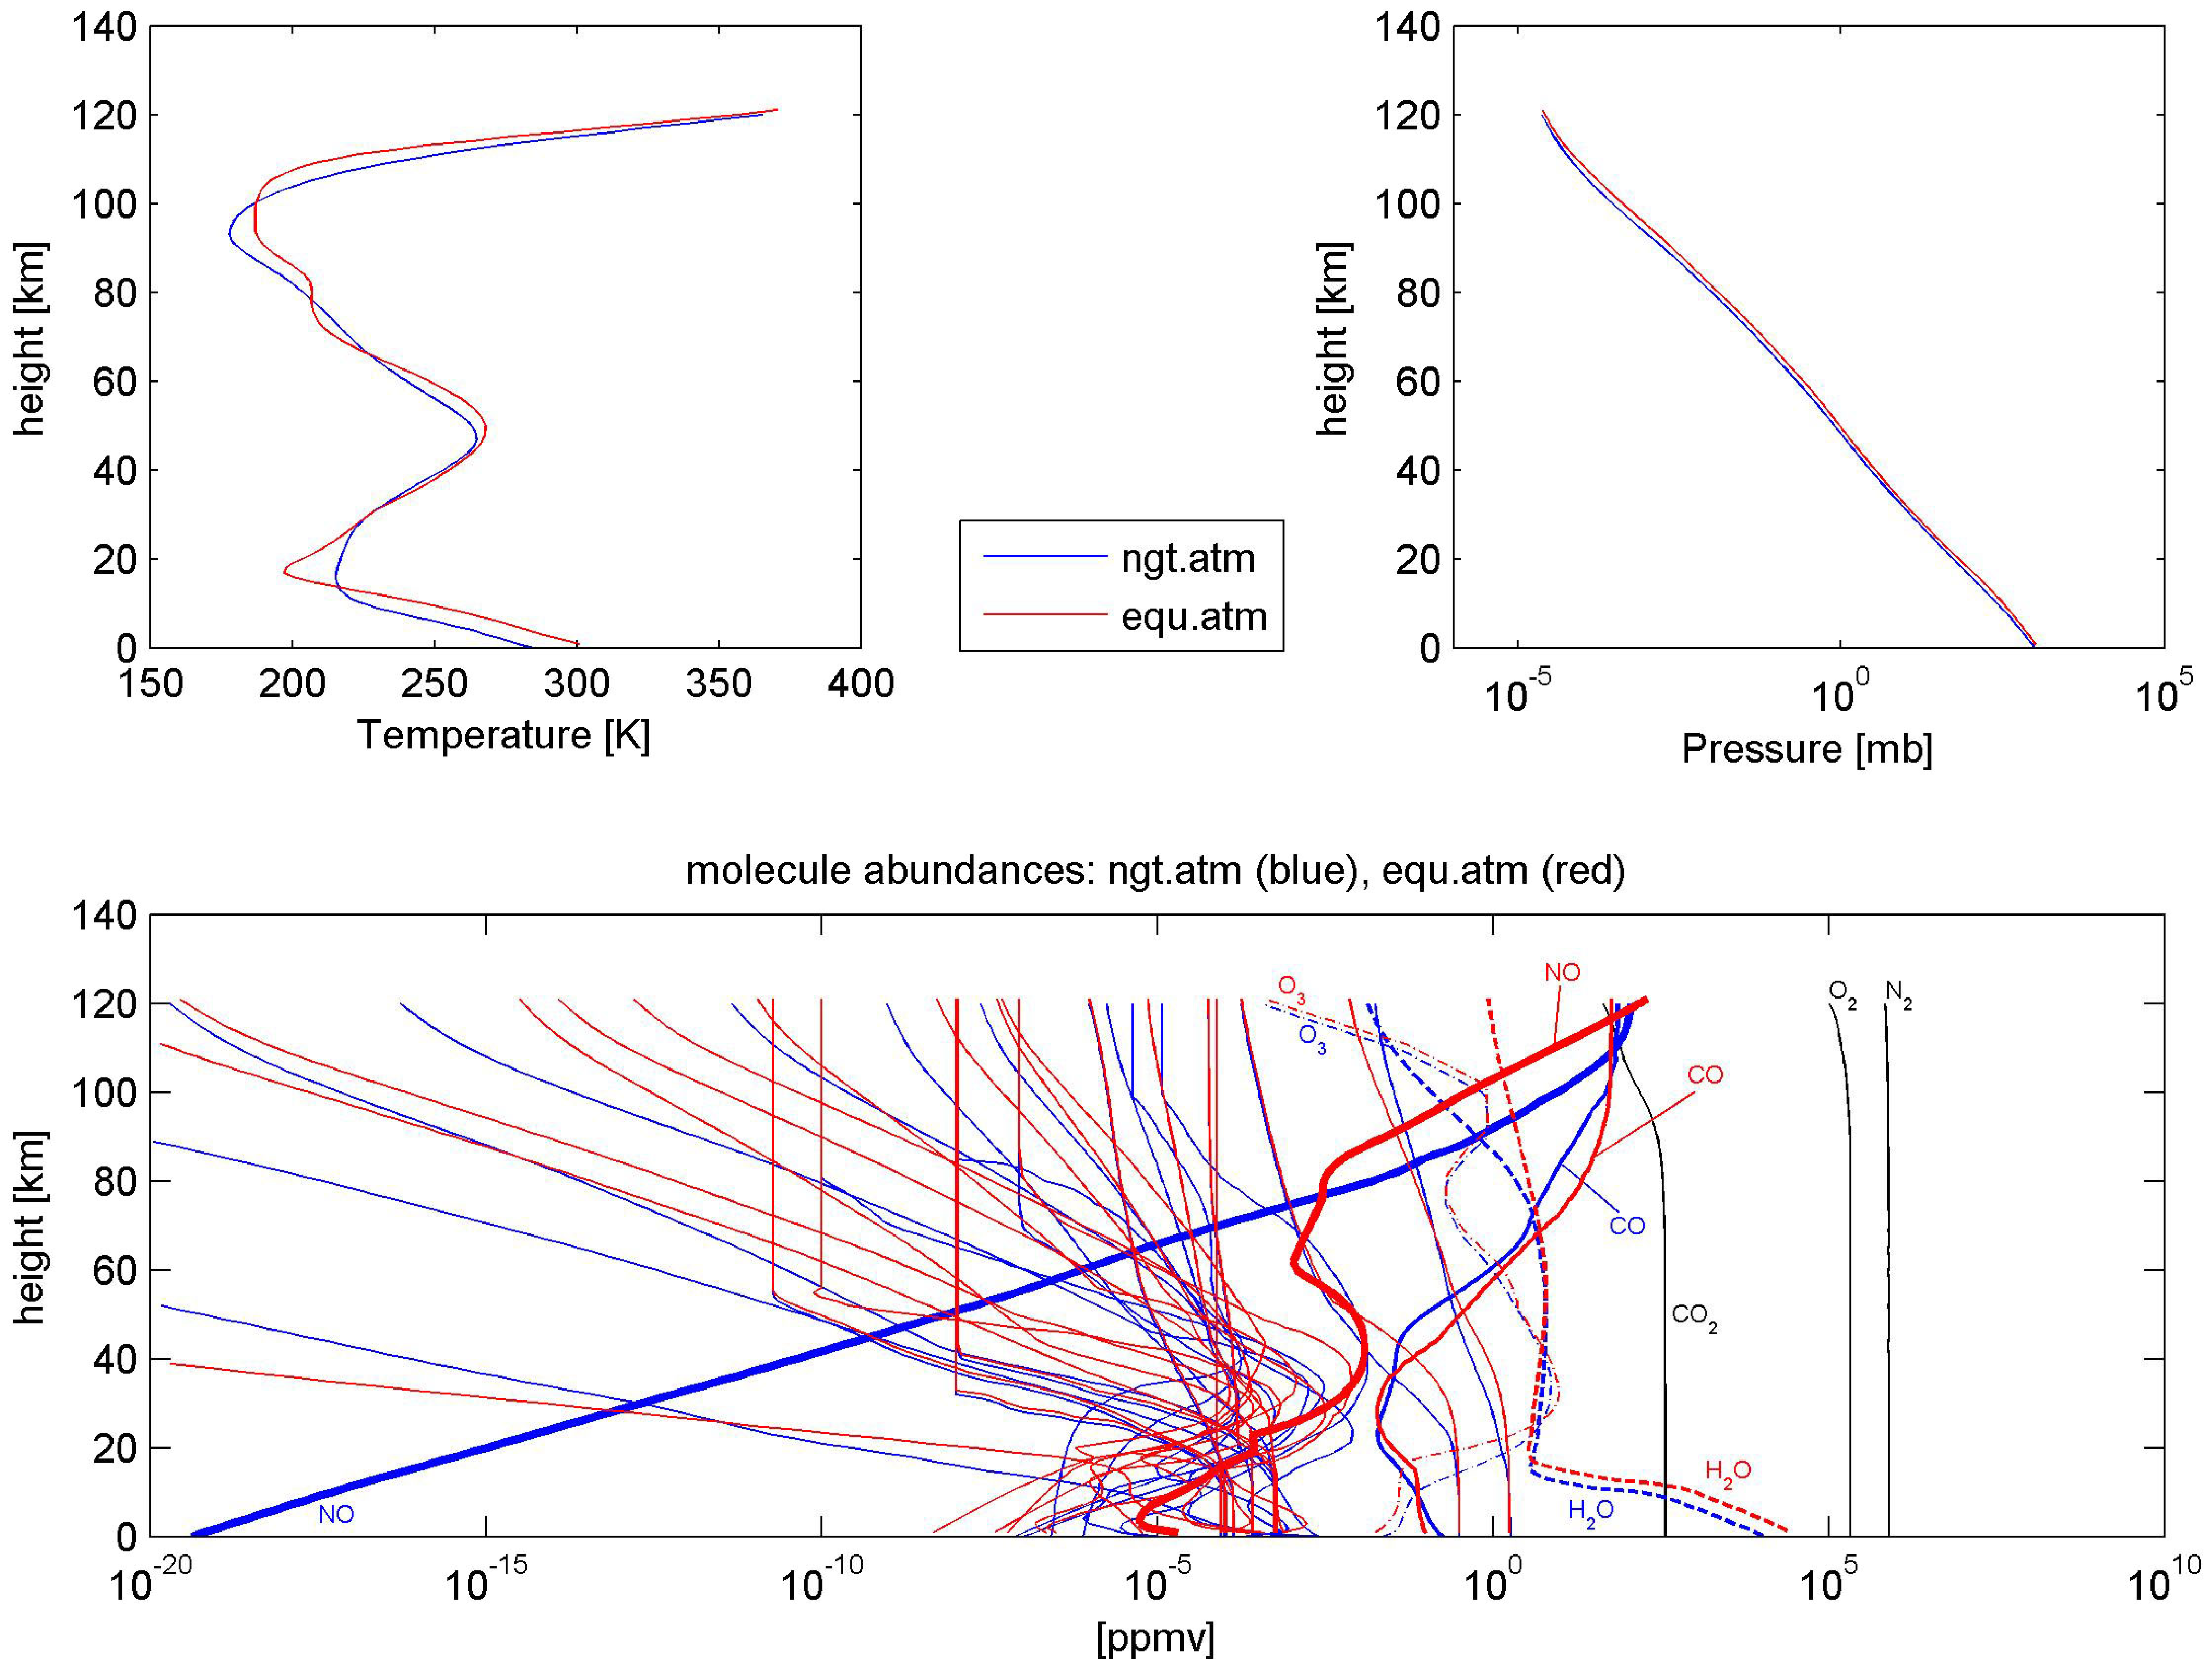
\psfig{file=figures/ngt_equ.eps,width=1.0\textwidth}
    \caption{Comparison of the equatorial (\tt equ.atm\rm) and the mid-latitude
    night time atmospheric profile (\tt ngt.atm\rm). Red lines correspond to
    the equatorial, blue lines to the mid-latitude profile.}
    \label{fig:std_atm_comp}
  \end{center}
\end{figure}
%-------------------------------------------------------------------------------
\begin{figure}[ht]
  \begin{center}
    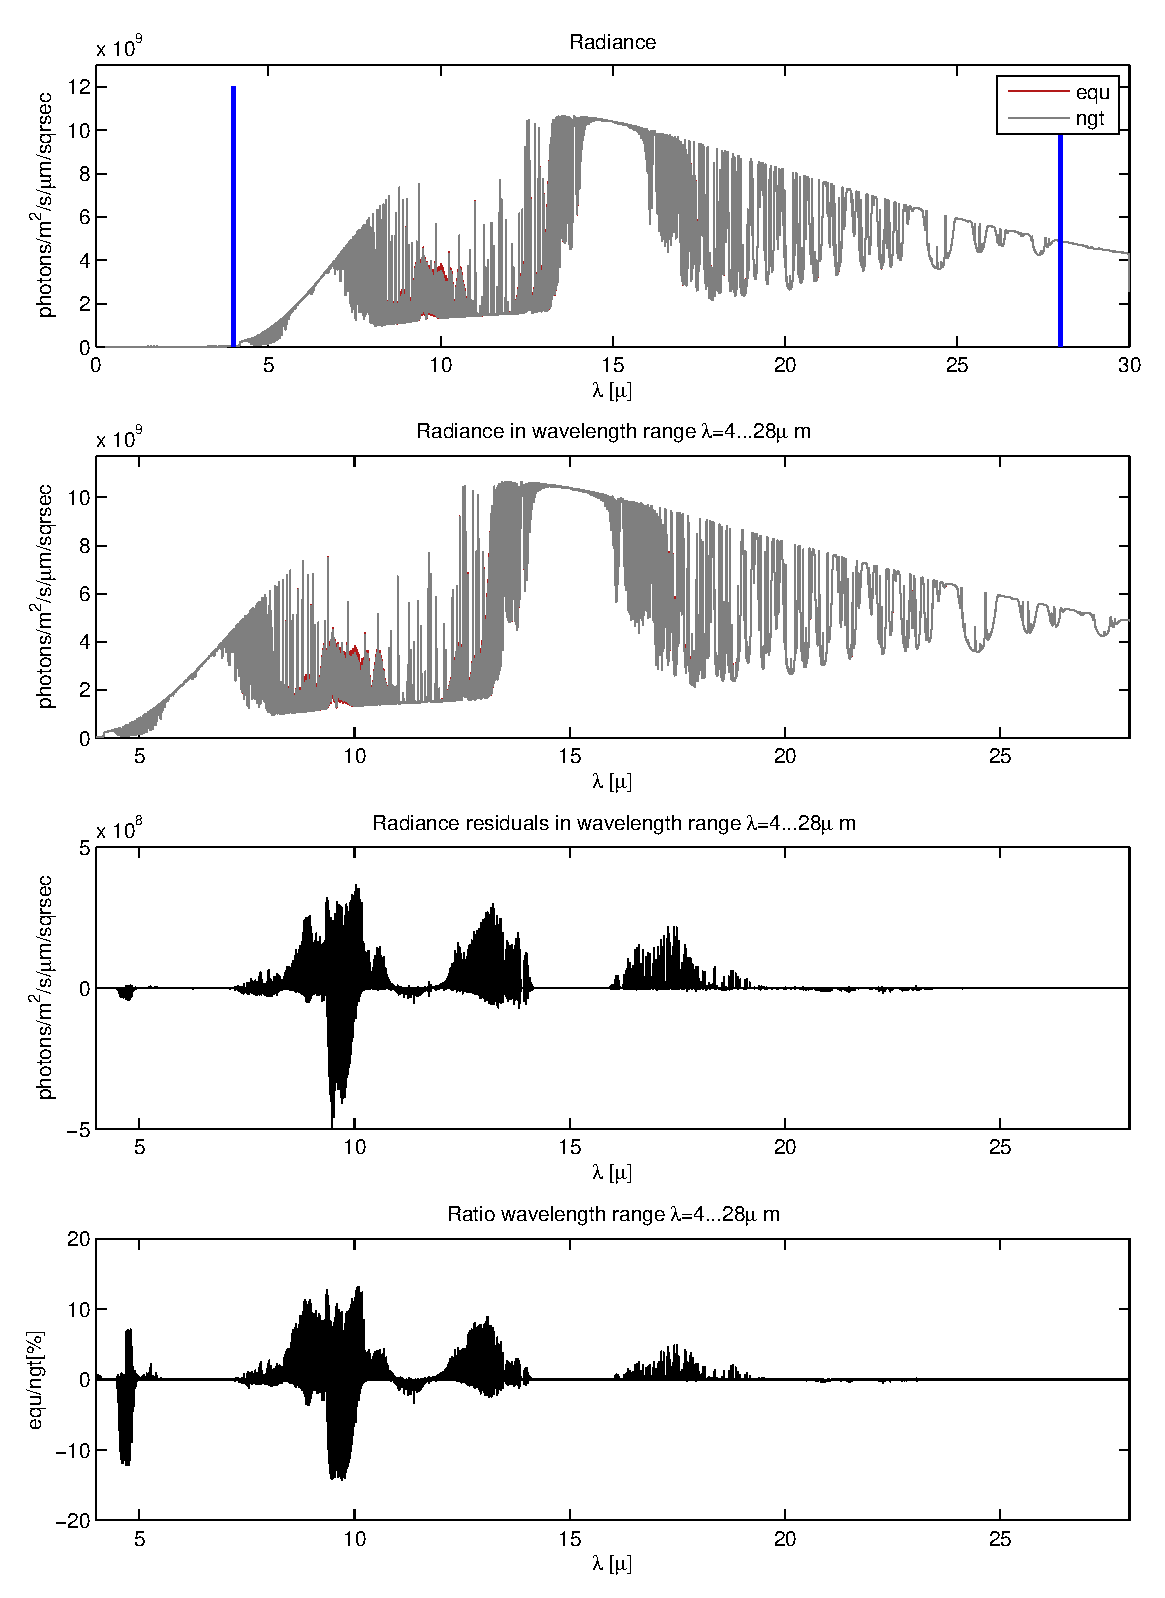
\psfig{file=figures/equ_ngt_4-28mu_rad.eps,width=0.75\textwidth}
    \caption{Direct comparison between the radiance spectra of equatorial day
    time (red line) and mid-latitude night time atmospheric standard profile
    (grey line) over the entire wavelength range $\lambda = 0.3 - 30$\,\mum{}
    (top panel). Blue lines mark the wavelength range
    ($\lambda = 4 - 28$\,\mum) plotted in the three panels below. {\it Second
    panel}: Same as in top panel, but for the limited wavelength range.
    {\it Third and bottom panel}: Residuals equ-ngt and ratio equ/ngt of the
    radiance spectra, respectively.}
    \label{fig:stdcomp_4-28_R}
  \end{center}
\end{figure}
%-------------------------------------------------------------------------------
\begin{figure}[ht]
  \begin{center}
    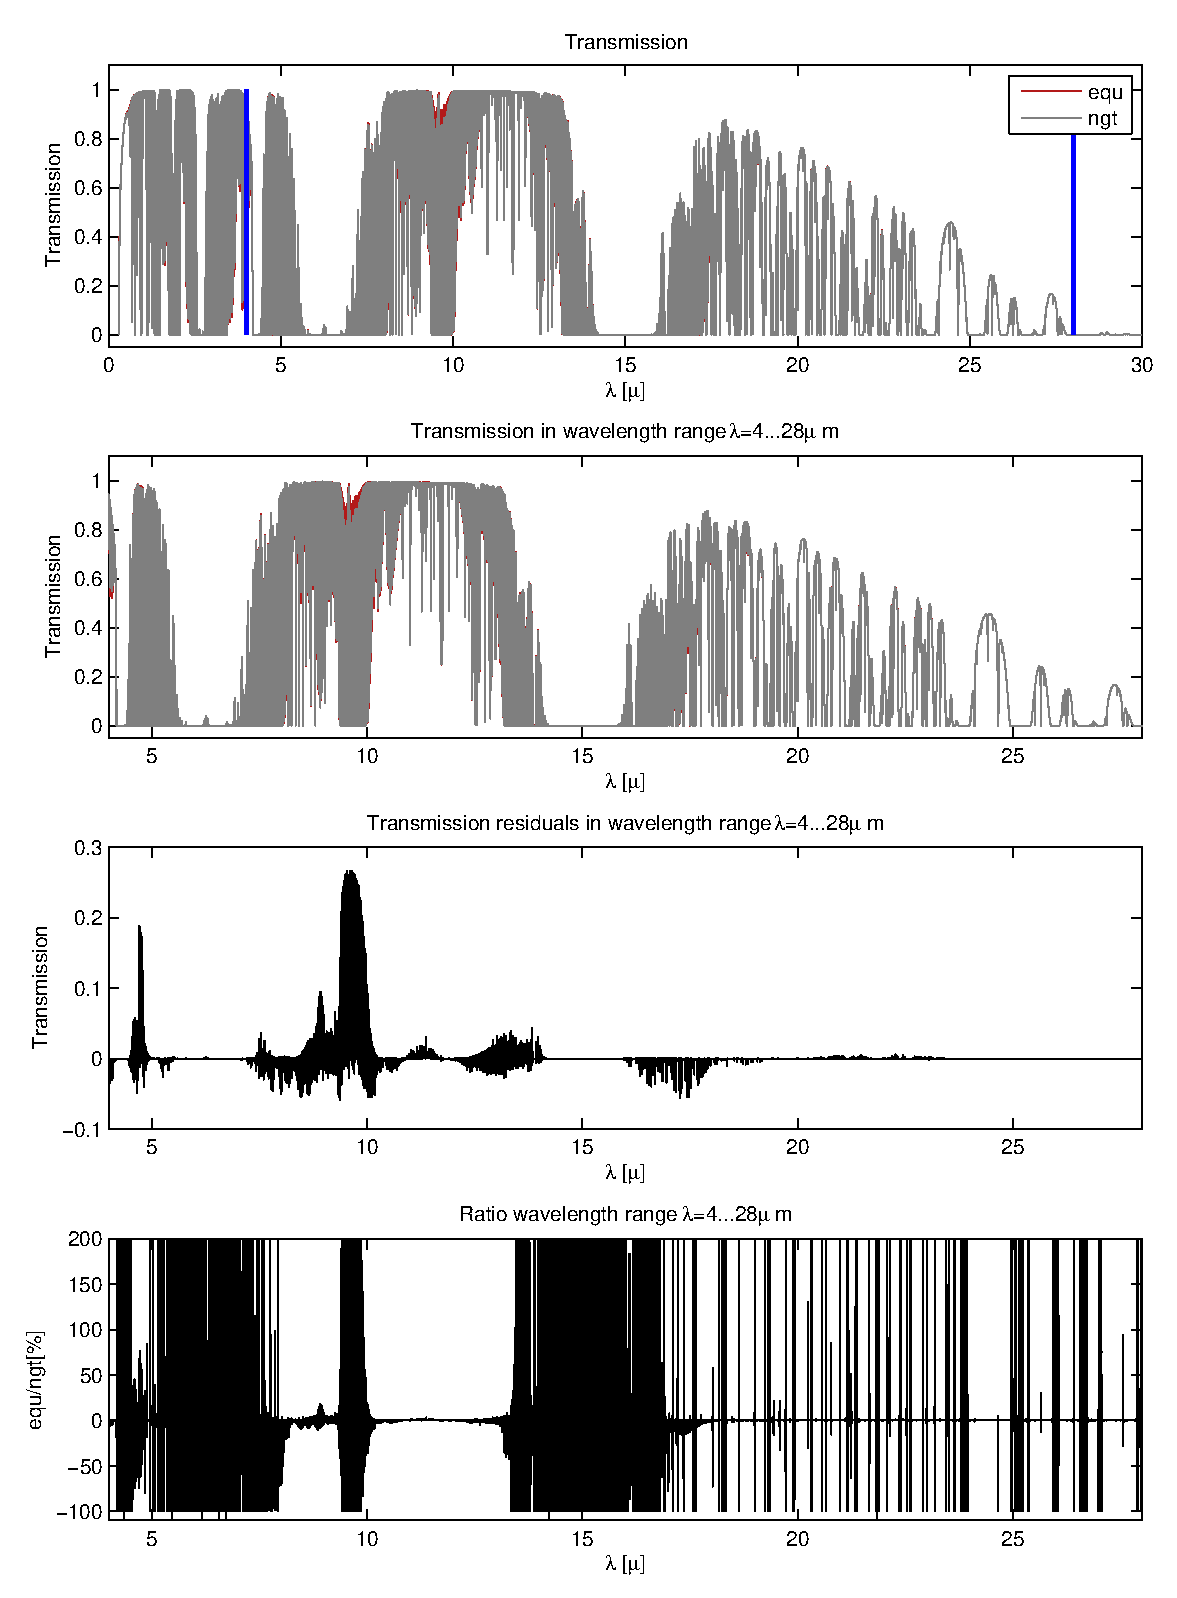
\psfig{file=figures/equ_ngt_4-28mu_tra.eps,width=0.75\textwidth}
    \caption{Same as Figure~\ref{fig:stdcomp_4-28_R}, but for the
    transmission.}
    \label{fig:stdcomp_4-28_T}
  \end{center}
\end{figure}
%-------------------------------------------------------------------------------

\clearpage

%-------------------------------------------------------------------------------
\subsubsection{GDAS profiles}\label{sec:gdas}
%-------------------------------------------------------------------------------
The \ac{GDAS} data provided by \ac{NOAA} are a model-based set of
meteorological data dedicated to weather forecast studies. The models are
archived by the \ac{ARL}, as a global, 1~degree latitude/longitude data set
based on pressure surfaces (starting from Dec.~2004). Apart from various
meteorological parameters for the surface, vertical profiles for 23 pressure
levels ranging from 0 to about 26\,km are provided for the geopotential height,
temperature, relative humidity, and wind components (not used in \mf) for three
dimensions. An example is shown in Figure~\ref{fig:gdas}.

%-------------------------------------------------------------------------------
\begin{figure}[ht]
  \begin{center}
    \begin{quote}
      \begin{small}
        \begin{verbatim}
# P[hPa] HGT[km] T[K]   RELHUM[%]
    903   0.971  294.5   49.9
    900   0.976  295.8   35.5
    850   1.467  293.7   30.9
    800   1.985  291.0   29.8
    750   2.533  288.2   27.4
    700   3.112  284.5   26.0
    650   3.726  280.7   18.8
    600   4.379  276.2   11.4
    550   5.077  271.4    8.7
    500   5.827  266.0    7.5
    450   6.638  259.9    7.5
    400   7.522  252.7   10.5
    350   8.494  244.7   25.1
    300   9.578  236.0   53.4
    250  10.813  227.0   66.5
    200  12.267  218.8   37.7
    150  14.069  209.2   17.3
    100  16.489  200.3   32.4
     50  20.571  206.1    0.0
     20  26.324  221.4    0.0
        \end{verbatim}
      \end{small}
    \end{quote}
    \caption{{\it GDAS profile} with columns for pressure, geoelevation,
    temperature, and relative humidity.}
    \label{fig:gdas}
  \end{center}
\end{figure}
%-------------------------------------------------------------------------------

The \mf\ software package provides the entire \ac{GDAS} data for the location
of Cerro Paranal from Dec.~2004 to Sep.~2013 on a 3\,h basis taken from the
\ac{NOAA}
archive\footnote{ \tt ftp://arlftp.arlhq.noaa.gov/pub/archives/gdas1/}.
Later dates (on a 6\,h basis) or data for a different site are automatically
downloaded from an online
archive\footnote{\tt http://nomad1.ncep.noaa.gov/pub/gdas/rotating/}.

%\clearpage

%-------------------------------------------------------------------------------
\subsubsection{ESO Meteo Monitor}\label{sec:emm}
%-------------------------------------------------------------------------------
The \ac{EMM} provides information on the local meteorological conditions at the
ESO sites La~Silla and Paranal. The data at Paranal are taken by a local meteo
station mounted on a 30\,m high mast installed in October 1984
\cite{meteomonitor}. This meteo station provides the following meteorological
information on a 20\,min average basis:

\begin{verbatim}
s1,d1 = wind speed (m/s) and direction (0=North, 90=East..)
        at 10m above ground (30m from 1998 onwards)
   rh = relative humidity (%) at 2m above ground
   t1 = air temperature (Celsius) at 2m above ground
   p  = pressure (mb) at 2m above ground
   td = dew point temperature (C) computed from rh and t1
\end{verbatim}

Starting from January 1st 1985, currently $\sim 400\,000$ data points are
measured with the following accuracy \cite{meteomonitor}:

\begin{verbatim}
wind direction: ~5.63deg
wind speed:     ~2% over 10m/s
temperature:    ~0.1deg
humidity:       linearity about 1%
seeing:         better than 10% above 0.25 arcsec
\end{verbatim}

The data can be retrieved online\footnote{\tt
http://archive.eso.org/asm/ambient-server} on a daily basis, or as download
provided by M.~Sarazin\footnote{\tt
http://www.eso.org/gen-fac/pubs/astclim/paranal/database/} and are
cumulatively shown in Figure~\ref{fig:meteomonitor}. Thus, for any requested
average time interval, like \eg\ December and January, ample measurements are
available. In compiling these data, care has to be taken to remove bad
measurements before further processing.

%-------------------------------------------------------------------------------
\begin{figure}[ht]
  \begin{center}
    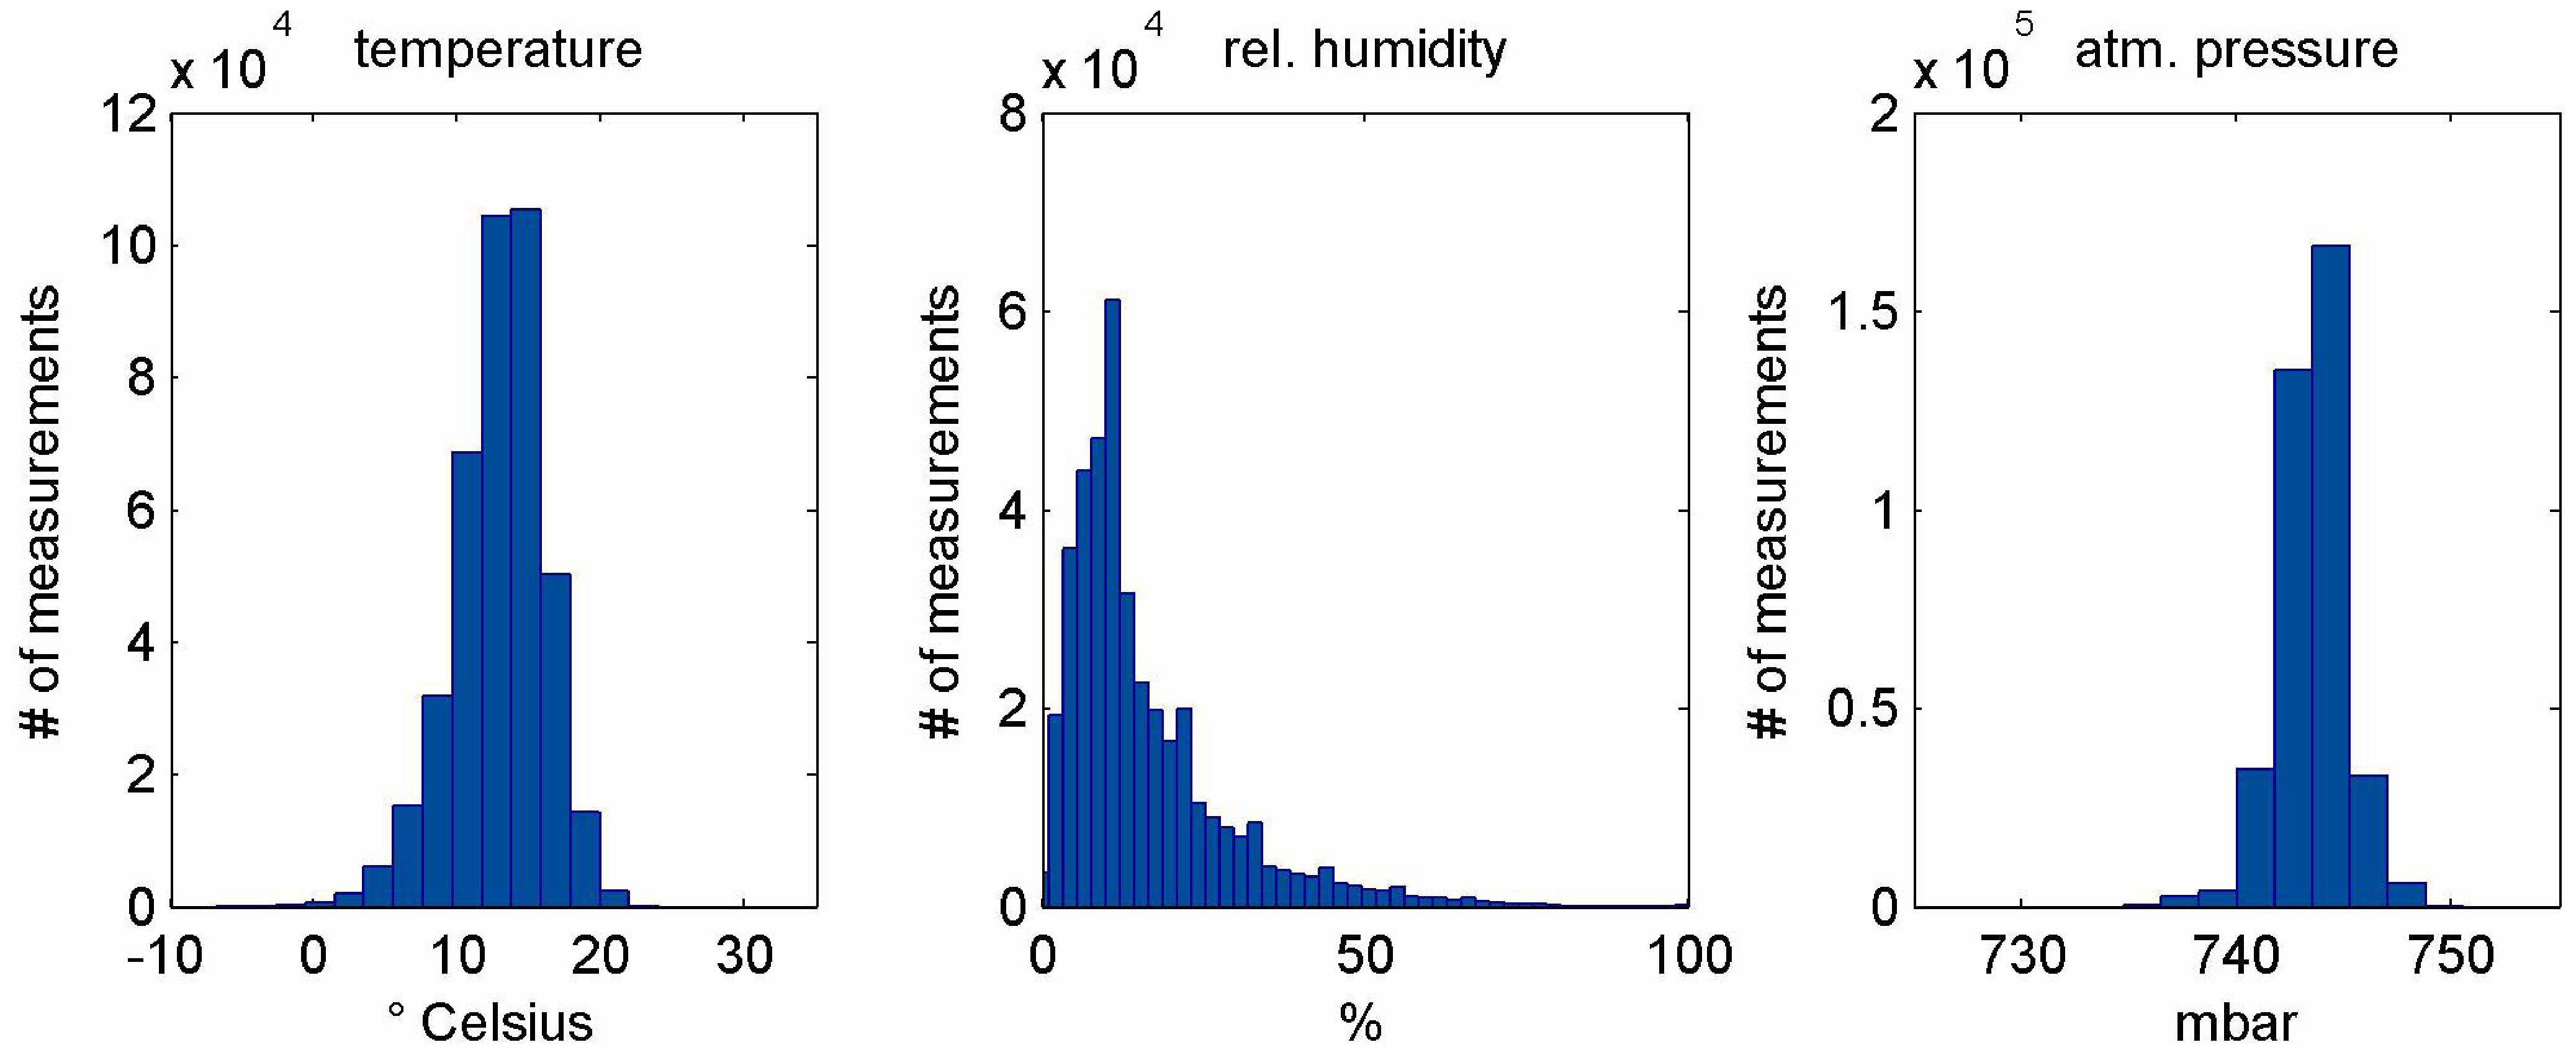
\psfig{file=figures/meteomonitor.eps,width=1.0\textwidth}
    \caption{Histograms of \ac{EMM} data (from Jan.~1985 to Jan.~2008).
{\it Left panel}: temperature; {\it middle panel}: relative humidity;
{\it right panel}: pressure.}
    \label{fig:meteomonitor}
  \end{center}
\end{figure}
%-------------------------------------------------------------------------------

\clearpage

%-------------------------------------------------------------------------------
\subsubsection{Processing of ESO Meteor Monitor data, GDAS, and MIPAS profiles}
\label{sec:processing}
%-------------------------------------------------------------------------------
The main disadvantage of the \ac{GDAS} profiles is that they do not represent
the local atmospheric conditions of the geographical position and height of the
observing site as accurately as provided by the \ac{EMM}, and even more so for
the MIPAS profiles. Therefore, one has to investigate how the three sources of
information can be merged into a single profile.

%-------------------------------------------------------------------------------
\paragraph*{GDAS profile processing}
\label{sec:gdas_processing}
%-------------------------------------------------------------------------------
The \ac{GDAS} profiles originate from a server at
\ac{NOAA}\footnote{http://140.90.198.158/pub/gdas/rotating/}. They are
retrieved via a dedicated software package \ac{GRIB} (see
Section~\ref{sec:installation}). \ac{GRIB} downloads a large data set
containing the specific \ac{GDAS} information for the requested point in time.
As this data set contains a model for the complete globe, subsequently, the
data points for the specified geolocation are extracted. Moreover, as the
\ac{GDAS} data are taken on a 3\,hr basis only, two profiles need to be
retrieved surrounding the requested point in time. The parameters
{\sc obsdate}, {\sc utc}, {\sc longitude}, and {\sc latitude} are required for
this task (see Section~\ref{sec:params}). They are usually provided by standard
and ESO FITS keywords. In the following, we will describe how the resulting two
profiles are combined to best match the date of the observations.

% As the download process from the web-server via \ac{GRIB} takes a considerable
% amount of time, \mf\ relies on two additional mechanisms to speed up the
% process. First of all, as the user works with his/her data set, the downloaded
% profiles are stored at a common location in the \mf\ directory tree
% (\verb|data/profiles/grib/| in {\sc basedir}, see Section~\ref{sec:params}).
% On subsequent calls of the routine, this location is first checked for the
% existence of the proper \ac{GDAS} profiles. 
If the profiles exist locally, no
download from the web-server is required. In addition, the \mf\ software
distribution contains a compilation of all Cerro Paranal \ac{GDAS} profiles for
the dates from Dec.~01, 2004 to Sep.~30, 2013. Thus, before requesting the data
from the web-server (in the case that they do not exist locally already), this
database is checked for the existence of the appropriate profiles. For
updates of this data set and the retrieval of data for other observing sites,
see Section~\ref{app:gdas}.

Unfortunately, the web-server does not provide \ac{GDAS} profiles for all
dates. Therefore, \mf\ incorporates a fall-back alternative to ensure
availability of \ac{GDAS} data in all occasions. To that end, the monthly
averaged profiles from the Cerro Paranal sky model are included as well (for a
detailed description see \cite{SM01UM} and Noll et al. \cite{NOL12}). If after
checking the local database or the web-server, a profile is still missing, the
best-matching profile for the two-month bins Dec.-Jan., Feb.-Mar., ...~are
taken. This is also done if the site is not Cerro Paranal.

The described procedure for the \ac{GDAS} profile retrieval is performed if
the parameter {\sc gdas\_prof} (see Section~\ref{sec:params}) is set to
``auto'', which is the default. As an alternative, a specific GDAS-like
profile (see Table~\ref{fig:gdas}) might be provided. Finally, it is possible
to avoid the use of GDAS profiles by setting {\sc gdas\_prof} to ``none''.

%-------------------------------------------------------------------------------
\paragraph*{Time averaged profiles}
\label{sec:time_average}
%-------------------------------------------------------------------------------
Typically, the requested observation date does not fall exactly onto a single
\ac{GDAS} time slot. Instead of simply retrieving the closest dataset the two
neighbouring profiles are obtained. In order to combine the two, a
time-weighted average is calculated, \ie\ performing a linear interpolation.

%-------------------------------------------------------------------------------
\paragraph*{Merging GDAS and MIPAS profiles}
\label{sec:gdas_mipas_merging}
%-------------------------------------------------------------------------------
Next, the resulting \ac{GDAS} profile is merged with the MIPAS standard
profile. To that end, the MIPAS profile is regridded to a new irregular height
grid with 50 levels (see Figure~\ref{fig:profile_levels}) spanning the whole
geoelevation range from 2-120\,km for Cerro Paranal. The \ac{GDAS} profile is
regridded to the same grid in the range 2-26\,km and then used to substitute
the respective columns in the MIPAS profile. In addition, the four height
levels from 20-26\,km are not only a simple substitute of the MIPAS data, but a
weighted mix of \ac{GDAS} and MIPAS profile, in order to provide a smooth
transition from one dataset to the other. The influence of the \ac{GDAS}
profile decreases with increasing height: 80\%, 60\%, 40\%, 20\% at 20\,km,
22\,km, 24\,km, 26\,km, respectively. Beyond 26\,km, no \ac{GDAS} information
is available.

The discussed fixed grid of layers is used if the parameter {\sc layers}
(see Section~\ref{sec:params}) is set to 1, which is the default. A value of
0 will cause the building of a natural grid consisting of all layers of the
MIPAS and the \ac{GDAS} profile. If local meteo data are used, the observer
altitude {\sc geoelev} is also added. The transition from \ac{GDAS} to MIPAS
is performed by means of a decrease of the relative difference of pressure,
temperature, and water vapour concentration of both profiles at the height of
the uppermost valid GDAS layer up to an altitude which is 1.2 times higher.
The resulting grid of layers is (slightly) more accurate than the fixed grid,
but also consists of a significantly higher number of levels.

%-------------------------------------------------------------------------------
\begin{figure}[ht]
  \begin{center}
    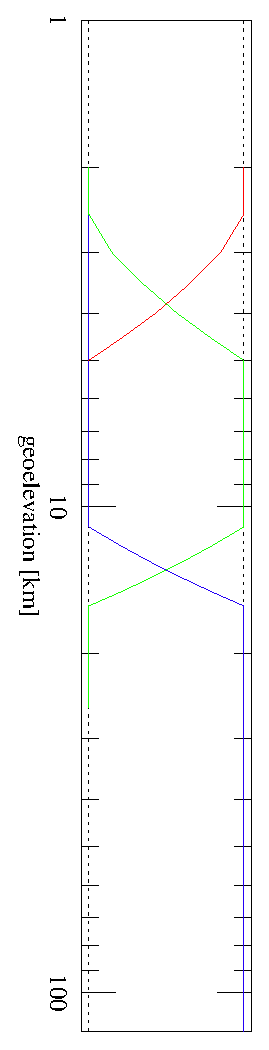
\psfig{file=figures/profiles.eps,height=1\textwidth,angle=90}
    \caption{{\it Composition of atmospheric profile:} relative importance of
    EMM data (red), \ac{GDAS} data (green) and MIPAS data (blue) as function of
    geoelevation. Note that the interface boundary of \ac{GDAS} and MIPAS data
    varies depending on the availability of the \ac{GDAS} data.}
    \label{fig:profile_levels}
  \end{center}
\end{figure}
%-------------------------------------------------------------------------------

%-------------------------------------------------------------------------------
\paragraph*{Combining GDAS/MIPAS profiles with EMM data}
\label{sec:emm_data}
%-------------------------------------------------------------------------------
Observed data from ESO telescopes provide on-site measurements at the ground
layer for pressure, temperature, and humidity originating from the ESO meteo
monitor at Cerro Paranal. A detailed study of the \ac{GDAS} data (see
Figure~\ref{fig:gdas_wind}), which represent the local troposphere, including
information concerning the dominant wind direction as a function of altitude
reveals a gradual reversal (rotation of 180$^\circ$) at a geoelevation of
5\,km, the so-called mixing altitude $h_{\mathrm{mix}}$ (see \cite{SM01UM}).
Beyond this altitude, the wind direction remains constant independent of the
observation date. Thus, it can safely be assumed that at this altitude the
influence of the local environment (as determined from the \ac{EMM} data) has
diminished.

In order to smoothly integrate the \ac{EMM} data, all \ac{GDAS} values for
pressure, temperature, and humidity below the altitude of the observatory are
set to the \ac{EMM} value. Values above the aforementioned mixing altitude are
left untouched. Intermediate values are linearly interpolated resulting in a
smooth transition. To this end, first, a logarithmically interpolated value of
the \ac{GDAS} data corresponding to the observatory's altitude $h_{\mathrm{tel}}$
is calculated for pressure, temperature, and humidity. These values describe
the reference point for the linear decrease of the relative difference between
\ac{EMM} and \ac{GDAS} data and in the interval $h_{\mathrm{tel}}-h_{\mathrm{mix}}$.

The resulting profile is a smooth combination of all input data, \ie\ MIPAS,
\ac{GDAS}, and \ac{EMM}.

The default mixing altitude of 5\,km can be manipulated by changing the
parameter {\sc emix} (see Section~\ref{sec:params}). This could be interesting
for other observing sites. Setting {\sc emix} to a value lower than the
observer altitude {\sc geoelev} causes a profile building without local meteo
data. In this case, the parameters {\sc pres}, {\sc temp}, and {\sc rhum} are
ignored.

%-------------------------------------------------------------------------------
\begin{figure}[ht]
  \begin{center}
    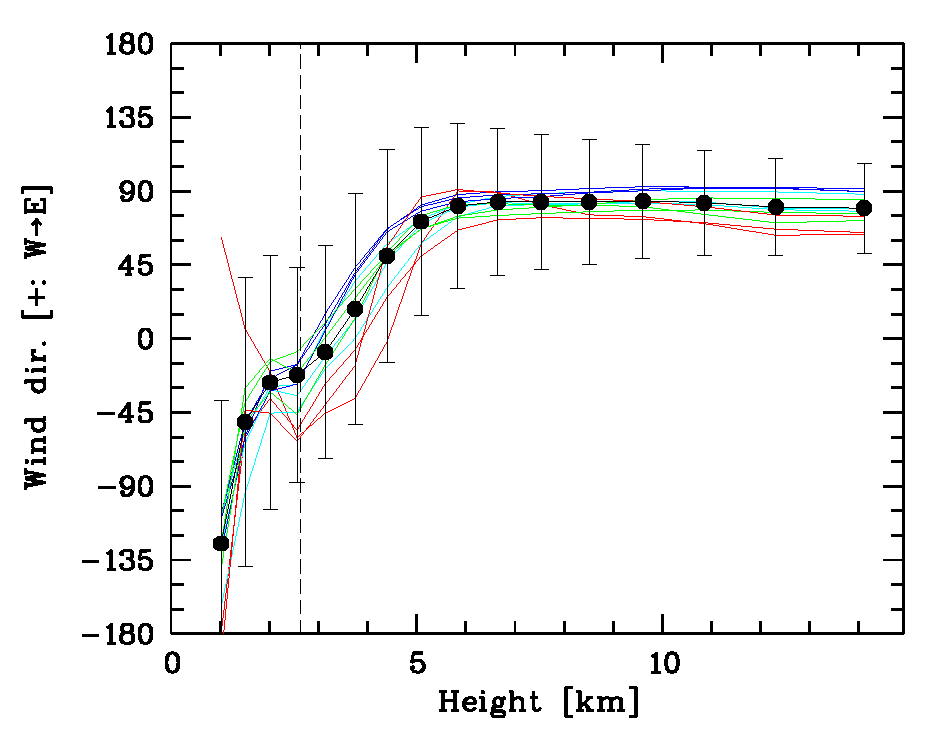
\psfig{file=figures/gdas_wdir_height_v.eps,width=0.7\textwidth}
    \caption{{\it \ac{GDAS} wind direction as function of geoelevation:} red,
cyan, blue, and green curves represent summer, autumn, winter, and spring,
respectively. The black symbols show the all year average with the
corresponding scatter. The vertical dashed line marks the geoelevation of
Paranal. At $\sim 5\,$km height, a constant plateau is reached.}
    \label{fig:gdas_wind}
  \end{center}
\end{figure}
%-------------------------------------------------------------------------------

%-------------------------------------------------------------------------------
\paragraph*{Scaling of the merged water vapour profile to a given PWV}
\label{sec:pwv_scaling}
%-------------------------------------------------------------------------------
The height profiles of the molecular abundances are defined by the atmospheric
standard profile. The only exception is water vapour, where the profile is a
combination of modelled and observed data as described above. The \ac{GDAS} and
\ac{EMM} data used cannot be controlled by the user. There might be cases where
this is not satisfying. For example, the user might be interested to use water
vapour columns derived from independent measurements for a better start
profile. For this purpose, \mf{} allows the user to enter a \ac{PWV} value
(parameter {\sc pwv}, see Section~\ref{sec:params}), which is used to scale the
merged water vapour profile. In this way, the input water vapour content of the
atmosphere can be fixed. Only the shape of the profile is then ruled by the
\ac{GDAS} and \ac{EMM} data. The profile scaling factor {\sc relcol}, which
is used in the context of the fitting procedure, refers to the modified
profile. By default, the {\sc pwv} option is switched off as indicated by a
value of -1.

%\clearpage

%-------------------------------------------------------------------------------
\subsection{Radiative transfer code}\label{sec:radcodes}
%-------------------------------------------------------------------------------
\mf\ uses the radiative transfer code Line-By-Line Radiative Transfer Model
(\lnflv{} / \lblrtmv), which is widely used in atmospheric and
climate research studies.

%-------------------------------------------------------------------------------
\subsubsection{Line File / Line-By-Line Radiative Transfer Model (LNFL/LBLRTM)}
\label{sec:lblrtm}
%-------------------------------------------------------------------------------
\ac{LBLRTM} is developed within the Radiative Transfer Working Group of the
\ac{AER} (see also Clough et al. \cite{CLO05}, \cite{AER}, and \cite{LBLRTM}).
It is publicly available. \ac{LBLRTM} can handle all molecules incorporated in
the {\tt aer\_v\_<version>} line parameter database \cite{LBLRTM} and offers a
wide range of possibilities to adjust input parameters (see
\cite{LBLRTM_instructions} for more details).

The \ac{AER} code package used here consists of two programmes: (a) the
"Line File" code \ac{LNFL}, which extracts user selected spectral lines from
the line parameter database, and provides these in appropriate form as input
for (b) the radiative transfer code \ac{LBLRTM}. Within \mf, the most recent
versions \lnflv{} and \lblrtmv{} are used.

Some \ac{LBLRTM} key features are (taken from \cite{LBLRTM}):

\begin{itemize}
  \item the Voigt line shape is used at all atmospheric levels with an
    algorithm based on a linear combination of approximating functions;
  \item it has been and continues to be extensively validated against
    atmospheric radiance spectra from the ultra-violet to the
    sub-millimeter;
  \item it incorporates the self- and foreign-broadened water vapour continuum
    model, MT\_CKD as well as continua for carbon dioxide, and for the
    collision induced bands of oxygen at 1600\,cm$^{-1}$ ($\lambda=6.25$\,\mum)
    and nitrogen at 2350\,cm$^{-1}$ ($\lambda=4.255$\,\mum);
  \item all parameters of the line database are used including the
    pressure shift coefficient, the halfwidth temperature dependence, and the
    coefficient for the self-broadening of water vapour;
  \item a version of the Total Internal Partition Function (TIPS) programme is
    used for the temperature dependence of the line intensities;
  \item the effects of CO$_2$ line coupling are treated as first order with
    the coefficients for carbon dioxide generated from Niro et al.
    \cite{NIR05};
  \item temperature dependent cross section data such as those available with
    the {\tt aer\_v\_<version>} database may be used to treat the absorption
    due to heavy molecules, \eg\ the halocarbons;
  \item an algorithm is implemented for the treatment of the variation of the
    Planck function within a vertically inhomogeneous layer as discussed in
    Clough et al. \cite{CLO92};
  \item algorithmic accuracy of \ac{LBLRTM} is approximately 0.5\% and the
    errors associated with the computational procedures are of the order of
    five times less than those associated with the line parameters so that the
    limiting error is that attributable to the line parameters and the line
    shape;
  \item its computational efficiency mitigates the computational burden of the
    line-by-line flux and cooling rate calculation (Clough et al.
    \cite{CLO92}), for example linear algebraic operations are used
    extensively in the computationally intensive parts of \ac{LBLRTM} so that
    vectorisation is particularly effective with a typical vectorised
    acceleration of 20;
  \item FFT instrument function with a choice of 9 apodisation functions;
  \item includes a realistic spectral sea surface emissivity model in the
    infrared (Masuda et al. \cite{MAS88}; Wu\&Smith \cite{WUS97});
  \item input atmospheric profiles in either altitude or pressure coordinates;
  \item interfaces with other radiative transfer models (like RRTM), and also
    the forward model for inversion algorithms (\eg\ Tropospheric Emission
    Spectrometer (TES) and Infrared Atmospheric Sounding Interferometer
    (IASI));
  \item these attributes provide spectral radiance calculations with
    accuracies consistent with the measurements against which they are
    validated and with computational times that greatly facilitate the
    application of the line-by-line approach to current radiative transfer
    applications.
\end{itemize}

In principle, the user can change the setup of the \ac{LBLRTM}. A reduced but
well documented list of input parameters and their default values is given by
the file ``config/lblrtm\_setup''. Some parameters are not fixed. They are
updated by other input data. For example, the wavelength range is given by
the input spectrum and possible cuts provided by the driver file (see
Section~\ref{sec:params}). A change of the fixed \ac{LBLRTM} input parameters
is only recommendable for those users, which have a very good knowledge of the
physics of atmospheric radiative transfer and/or \ac{LBLRTM}.

%-------------------------------------------------------------------------------
\subsubsection{{\tt aer} line database}\label{sec:molecs}
%-------------------------------------------------------------------------------
For calculating molecular spectra, the {\tt aer\_v\_<version>} database
\cite{LBLRTM} is used. It is built from \ac{HITRAN}~2008 \cite{HITRAN} and
contains several updates. Currently, it covers the full spectral range from
$0 - 25,232$\,cm$^{-1}$ (\ie\ up to $0.4\,\mu$m) provides spectral information
for 42 molecules. In total, more than 2,700,000 spectral lines are included.
The majority is based on modelled data. However, only those 30 molecules are
taken into account, which are present in the atmospheric standard profile. The
remaining ones are minor trace gases and do not contribute significantly
neither to radiance, nor transmission spectra (see Section~\ref{sec:spectra}).
Table~\ref{sec:molecs} provides an overview of all molecules based on the
{\tt aer} database (and known by \ac{LBLRTM}) and those contained in the
standard atmospheres (Column~4).

\begin{table*}[!ht]
\begin{center}
\caption{List of molecules as provided by the {\tt aer} line parameter database}
\label{tab:molecs}
\vspace{6pt}
\centering
\begin{tabular}{r | c | c | c | c}     % 5 columns
\hline\hline
\# of molecule & molecule & alt. name & std. atmosphere & \ac{LBLRTM} \\
\hline
1 & H$_2$O & Water & X & X \\
2 & CO$_2$ & Carbon dioxide & X & X \\
3 & O$_3$  & Ozone & X & X \\
4 & N$_2$O & Nitrous oxide & X & X \\
5 & CO  & Carbon monoxide & X & X \\
\hline
6 & CH$_4$ & Methane & X & X \\
7 & O$_2$  & Oxygen & X & X \\
8 & NO  & Nitric oxide & X & X \\
9 & SO$_2$ & Sulfur dioxide & X & X \\
10 & NO$_2$ & Nitrogen dioxide & X & X \\
\hline
11 & NH$_3$  & Ammonia & X & X \\
12 & HNO$_3$ & Nitric acid & X & X \\
13 & OH   & Hydroxyl &  & X \\
14 & HF   & Hydrogen fluoride &  & X \\
15 & HCl  & Hydrogen chloride &  & X \\
\hline
16 & HBr  & Hydrobromic acid &  & X \\
17 & HI   & Hydrogen iodide &  & X \\
18 & ClO  & Chlorine monoxide & X & X \\
19 & OCS  & Carbonyl sulfide & X & X \\
20 & H$_2$CO & Formaldehyde &  & X \\
\hline
21 & HOCl & Hypochlorous acid & X & X \\
22 & N$_2$   & Nitrogen & X & X \\
23 & HCN  & Hydrogen cyanide & X & X \\
24 & CH$_3$Cl & Chloromethane &  & X \\
25 & H$_2$O$_2$ & Hydrogen peroxide & X & X \\
\hline
26 & C$_2$H$_2$ & Acetylene & X & X \\
27 & C$_2$H$_6$ & Ethane & X & X \\
28 & PH$_3$  & Phosphine &  & X \\
29 & COF$_2$ & Carbonyl fluoride & X & X \\
30 & SF$_6$q  & Sulfur hexafluoride & X & X \\
\hline
31 & H$_2$S & Hydrogen sulfide  &  & X \\
32 & HCOOH & Formic acid &  & X \\
33 & HO$_2$ & Hydroperoxyl  &  & X \\
34 & O    & Oxygen &  & X \\
35 & ClONO$_2$q  &  & X & X \\
\hline
36 & NO+  & Nitrosonium &  & X \\
37 & HOBr &  &  & X \\
38 & C$_2$H$_4$ & Ethylene &  & X \\
39 & CH$_3$OH & Methanol &  & X \\
40 & BrO  &  &  & X \\
\hline
41 & C$_3$H$_8$ & Propane &  & X \\
42 & C$_2$N$_2$ & Cyanogen &  & X \\
\hline
\end{tabular}
\end{center}
\end{table*}

\clearpage

%-------------------------------------------------------------------------------
\subsection{Molecular spectra}\label{sec:spectra}
%-------------------------------------------------------------------------------
The process of fitting molecular spectra is a complex task, which requires
optimised input parameters. One of the key inputs for the fitting is the number
of molecules that are included in the fitting. Fewer molecules in the fitting
process result in the code finding a solution in significantly shorter amounts
of time. Also the fitting process is a lot more robust. However, if too few
molecules are included in the fit, the results may not provide a satisfying
residual for model and observation. Optimally, one should include exactly those
molecules in the fit, which will significantly contribute over the wavelength
range of interest.

To the end of providing some insight into what molecules are required for the
fit at a specific wavelength interval, in the following, we provide guidelines
with a specific focus on the test data provided with this software package for
the instruments CRIRES, VISIR, and X-Shooter (see Section~\ref{sec:pwv}).

We have computed spectra with \ac{LBLRTM} covering the complete wavelength
range from $0.3-30$\,\mum\ using all molecules (\ie\ C$_{2}$H$_{2}$,
C$_{2}$H$_{6}$, CH$_{4}$, CO$_{2}$, COF$_{2}$, CO, ClONO$_{2}$, ClO, F14,
H$_{2}$O$_{2}$, H$_{2}$O, HCN, HNO$_{3}$, HOCl, N$_{2}$O, N$_{2}$, NH$_{3}$,
NO$_{2}$, NO, O$_{2}$, O$_{3}$, OCS, SF$_{6}$, SO$_{2}$), individually, \ie\ one
at a time. At fixed wavelength, we have then calculated the normalised total
radiance/transmission (by summing up the contributions of all molecules and
subtracting the continuum) and the resulting relative importance of individual
molecules.

The Figures~\ref{fig:molecs_all}-\ref{fig:molecs_xshoo} shown in the Appendix,
give all molecules that, over the displayed wavelength range, exhibit at
fixed wavelength $\lambda$ a relative importance of at least 5\%. The molecular
data have been rebinned to 3000 data points for each individual wavelength
range. This results in a varying resolution and in more molecules becoming
important over smaller wavelength regimes. C$_{2}$H$_{6}$, \eg, has a few
significant lines in some of the wavelength ranges shown (\eg\
Figure~\ref{fig:molecs_crires}), but does not show up in the overview plot
(Figure~\ref{fig:molecs_all}). Typically, transmission (blue) and radiance
(red) plots do not differ significantly. Hence, we do not show them separately.
Note that these plots do not allow calculation of absolute fluxes.

These plots can be used to identify the important molecules over any wavelength
range. For the range shown in Figure~\ref{fig:molecs_crires}, \eg, the user
ought to include H$_{2}$O, CH$_{4}$, and O$_{3}$. The fitting might mildly profit
also from including C$_{2}$H$_{6}$.



%-------------------------------------------------------------------------------
\subsection{Thermal emission by telescope}\label{sec:greybody}
%-------------------------------------------------------------------------------
The telescope structure and the observing instrument cause unavoidable thermal
emission in the IR. In particular, the telescope main mirror is a significant
source of radiation. Hence, for radiance spectra, this background component has
to be considered. A simple approximation is the calculation of a grey body
spectrum, which equals a black body (BB) of temperature $T$ times a
wavelength-independent emissivity $\epsilon$. Since the emitting source, \ie\
the main mirror, also absorbs a fraction of $1 - \epsilon$ of the incoming
sky radiation, the relative contribution of the telescope emission to the
observed radiation is increased. Therefore, the apparent grey body radiation
in flux-calibrated spectra can be derived by
\begin{equation}
F_{\rm tel} = \frac{\epsilon}{(1 - \epsilon)} \,{\rm BB}(T).
\end{equation}
For $T$, \mf\ uses the temperature of the primary mirror (input parameter
{\sc m1temp}, see Section~\ref{sec:params}). Since the mirror temperature
is close to the ambient temperature of about 280-290\,K (Paranal), the grey
body emission is expected to be important at wavelengths longwards of the
$H$-band. The emissivity is a free fit parameter (see parameter {\sc telback}).
An initial value can be provided in the parameter file. The default value is
$0.1$.

%-------------------------------------------------------------------------------
\subsection{Adaptation of model to input spectrum}\label{sec:adaption}
%-------------------------------------------------------------------------------
A good correspondence of the calculated model spectrum and the observed
spectrum is usually prevented by the broadening of the spectral lines by the
instrument, small errors in the wavelength calibration, uncertainties in the
flux calibration in the case of emission spectra, or the non-flat standard star
continuum in the case of transmission spectra. Hence, these unavoidable
shortcomings of observed data have to be accounted for in the fitting
procedure. For this reason, \mf\ modifies the model spectrum using a
polynomial fit of the continuum and the wavelength grid. In addition, the model
gets convolved with a kernel mimicking the instrumental profile. In the
following, we discuss the fit parameters related to this adaptation process in
detail.

%-------------------------------------------------------------------------------
\subsubsection{The continuum}\label{sec:continuum}
%-------------------------------------------------------------------------------
The model spectrum is scaled by a polynomial of degree $n_\mathrm{c}$
({\sc cont\_n} in the parameter file; see Section~\ref{sec:params})
\begin{equation}
F_\mathrm{out}(\lambda) =
F_\mathrm{in}(\lambda) \, \sum_{i = 0}^{n_\mathrm{c}} a_i \lambda^i.
\end{equation}
For deriving the $n_\mathrm{c} + 1$ coefficients $a_i$, the zero point of the
wavelength grid is shifted to the centre of the fit range. For $a_0 = 1$ and
all other $a_i = 0$, the model spectrum remains unchanged. This is the default
configuration for the initial coefficients. In the parameter file, the
initial value of the constant term of the polynomial (parameter
{\sc cont\_const}) can be set manually. The continuum correction is carried
out independently for each fit range listed in the {\sc range\_include} file
if such a file is provided. A fit range (or the full spectrum) is further
split if it is distributed over more than one chip.

Before correcting the continuum, optionally a flux conversion is carried out.
Details on the options selected by the parameter {\sc flux\_unit} are given in
Section~\ref{sec:params}. If the required data units are not included in
{\sc flux\_unit}, this factor must be incorporated into the $a_0$ coefficient
of the polynomial. As a general rule, it is advisable to choose $a_0$ close to
the mean flux (emission) or maximum flux (transmission) of the input spectrum
(after consideration of {\sc flux\_unit}) to optimise the performance of \mf.

%-------------------------------------------------------------------------------
\subsubsection{The wavelength solution}\label{sec:wavegrid}
%-------------------------------------------------------------------------------
The wavelength grid of the model spectrum is adapted to that of the observed
spectrum by applying a Chebyshev polynomial of degree $n_\mathrm{w}$
({\sc wlc\_n} in the parameter file; see Section~\ref{sec:params})
\begin{equation}
\lambda' = \sum_{i = 0}^{n_\mathrm{w}} b_i t_i,
\end{equation}
where
\begin{equation}
t_i = \left\{ \begin{array}{ll}
1 & \textrm{for\ } i = 0 \\
\lambda & \textrm{for\ } i = 1 \\
2 \, \lambda \, t_{i-1} - t_{i-2} & \textrm{for\ } i \ge 2
\end{array} \right.
\end{equation}
and $\lambda$ ranging from -1 to 1. The temporary conversion of the wavelength
grid to a fixed interval results in coefficients $b_i$ independent of the
wavelength range and step size of the input spectrum. For $b_1 = 1$ and all
other $b_i = 0$, the model spectrum remains unchanged. This is the default
configuration for the initial coefficients. In the parameter file,
the initial value of the constant term of the polynomial (parameter
{\sc wlc\_const}) can be set manually. This parameter corresponds to a
wavelength shift relative to half the full wavelength range. For each chip or
FITS extension, the wavelength fit is carried out independently.

For checks or improvements of the input wavelength grid, the model wavelengths
rebinned to the input grid are provided in the results tables of \mf{} and
{\tt calctrans} (column ``mlambda'', see Section~\ref{sec:outputfiles}). The
wavelengths are always given in $\mu$m and vacuum. Note that the reliability of
this absolute wavelength calibration depends on the quality of the fit. Outside
the selected fitting ranges, the wavelengths have to be interpolated or
extrapolated by the Chebyshev polynomial. In particular, at optical and near-IR
wavelengths, where strong absorption bands suitable for fitting are rare, the
provided wavelengths have to be taken with care. For this reason, \mf{} does
not provide an automatic wavelength solution correction.

%-------------------------------------------------------------------------------
\subsubsection{The resolution}\label{sec:resolution}
%-------------------------------------------------------------------------------
The model spectrum is convolved with up to three different profiles in order to
get similar line shapes as in the observed spectrum. If a profile is not
desired, it can be skipped by setting its width and fit flag in the parameter
file to zero (see Section~\ref{sec:params}).

The first kernel is a simple boxcar
\begin{equation}
F_\mathrm{box}(\lambda) = \left\{ \begin{array}{ll}
1 & \textrm{for\ } -w_\mathrm{box}/2 \le \lambda \le w_\mathrm{box}/2 \\
0 & \textrm{for\ } \lambda < -w_\mathrm{box}/2 \cap \lambda > w_\mathrm{box}/2
\end{array} \right.
\end{equation}
which is adapted to the pixel scale and normalised to an integral of 1. In
the parameter file, the width $w_\mathrm{box}$ (parameter {\sc relres\_box}) has
to be given as fraction of the slit width, which is determined by the
parameters {\sc slitw}, the slit width in arcsec, and {\sc pixsc}, the pixel
scale in arcsec (see Section~\ref{sec:params}). By default, {\sc relres\_box}
is set to 1, \ie\ the slit width. The fit parameter {\sc relres\_box} can only
vary between 0 and 2.

The second convolution kernel is a Gaussian
\begin{equation}
F_\mathrm{gauss}(\lambda) = \frac{1}{\sigma \sqrt{2 \pi}}
\exp{\Bigg(-\frac{\lambda^2}{2 \sigma^2}\Bigg)}
\end{equation}
centred on 0, where
\begin{equation}
\sigma = \frac{w_\mathrm{gauss}}{2 \sqrt{2 \ln{2}}}.
\end{equation}
The FWHM $w_\mathrm{gauss}$ is given by the driver file parameter
{\sc res\_gauss} in pixels (see Section~\ref{sec:params}). It is restricted to
values below 100 pixels. The default value is 1 pixel. The number of pixels in
the kernel amounts to {\sc kernfac} (default: 3) times $w_\mathrm{gauss}$.

Finally, the third kernel is a Lorentzian
\begin{equation}
F_\mathrm{lorentz}(\lambda) = \frac{1}{\pi} \,
\frac{\lambda}{\lambda^2 + (w_\mathrm{lorentz}/2)^2}
\end{equation}
centred on 0, where $w_\mathrm{lorentz}$ is the FWHM. The width is adjusted by
the driver file parameter {\sc res\_lorentz}, which has to be provided in
pixels (see Section~\ref{sec:params}). It is restricted to values below 100
pixels. The default value is 1 pixel. The number of pixels in the kernel
amounts to {\sc kernfac} (default: 3) times $w_\mathrm{lorentz}$. Compared to a
Gaussian, the Lorentzian approaches the 0-level flux significantly slower, at
much larger distances from the maximum.

Note that width zero components can occur in typical conditions, \eg{} the line
profile is very close to a pure Lorentzian shape. If this is not intended, the
user should reduce the number of degrees of freedom by fixing individual fit
components. A zero here identifies a unity convolution (\ie{} no change
of the input spectrum).

The combination of a Gaussian and a Lorentzian is called a Voigt profile. The
flag {\sc kernmode} (see Section~\ref{sec:params}) allows the user to apply
only a single Voigt profile kernel, which is calculated by an approximate
formula that takes the FWHM of Gaussian and Lorentzian as input. In this case
({\sc kernmode} = 1), {\sc kernfac} gives the kernel size in FWHM of the
derived Voigt profile and not the FWHM of Gaussian and Lorentzian, as it is
done for the default mode of two independent convolutions ({\sc kernmode} = 0).
For the fit results, the {\sc kernmode} selection should be less important than
the relative contributions of boxcar, Gaussian, and Lorentzian to the fitted
line profile. Significant changes in the line profile can cause deviations in
the water vapour column of more than 10\% (cf. Section~\ref{sec:evaluation}).

The parameter {\sc varkern} allows the user to fit a kernel that linearly
increases with wavelength (see Section~\ref{sec:params}). If the flag is set to
1, this option is selected. It is suitable for dispersion-dominated kernels and
constant wavelength bins. In this case, the initial FWHM parameters are given
for the central wavelength of the full wavelength range (considering the data
of all chips). The default {\sc varkern}~=~0 assumes a constant kernel for the
entire wavelength range. This option is suitable for narrow wavelength ranges
and slit/object profile-dominated kernels.

Finally, the user can provide an optimised kernel by an ASCII file which is
provided by the parameter {\sc kernel\_file} (see Section~\ref{sec:params}).
If this option is used (\ie\ the default ``none'' is replaced by the
corresponding file name), the fixed input kernel overrules the creation of
a kernel based on boxcar, Gaussian, and Lorentzian components. Since there will
be no fit of the kernel shape and width, the line profile has to be known well.
Note that {\sc varkern}~=~1 will not have an effect, since the pixel-based
input kernel is wavelength independent.

\cleardoublepage
%-------------------------------------------------------------------------------
\section{Code performance}\label{sec:evaluation}
%-------------------------------------------------------------------------------
In the following, we illustrate the handling of \mf\ and the quality of the
resulting fits by means of several example spectra. In Section~\ref{sec:pwv},
the derivation of molecular abundances is discussed. In particular, the quality
of the derived water vapour column densities is investigated.
In Section~\ref{sec:tactest}, we briefly discuss the performance of \mf\ in
terms of the correction of telluric absorption features. Finally,
Section~\ref{sec:tips} provides some general rules that should be considered
for a successful application of \mf.

%-------------------------------------------------------------------------------
\subsection{Derivation of molecular abundances}\label{sec:pwv}
%-------------------------------------------------------------------------------
We illustrate the use of \mf\ for the derivation of molecular abundances by
means of a small sample of spectra consisting of a CRIRES, an X-Shooter, and
a pair of VISIR spectra (see Table~\ref{tab:sample}). The high-resolution
($R \approx 50000$) CRIRES standard star spectrum is typical of spectra that
are used for the nocturnal \ac{PWV} measurements at the VLT \cite{PWV}. Despite
of the narrow wavelength range from 3.274 to 3.352\,$\mu$m, the good resolution
allows one to fit many individual telluric absorption lines, which usually
results in convincing fits of the water vapour content and abundances of other
significant molecules in the atmosphere. The medium-resolution
($R \approx 8800$) X-Shooter VIS-arm star spectrum demonstrates \cite{PWV}
measurements in a narrow wavelength range at relatively short wavelengths
(0.940 to 0.951\,$\mu$m). Finally, the VISIR LR-mode spectra
($R \sim$ a few hundred) are examples for sky radiance spectra in the mid-IR
that are dominated by water vapour emission (see Section~\ref{sec:spectra}).
Since the very low resolution is not optimal for deriving \ac{PWV} values,
these spectra can be used to test the limits of the method. The presence of
spectra that were taken at similar time but for different wavelength regimes
allows some interesting comparisons.

\begin{table*}
\caption[]{Description of test sample}
\label{tab:sample}
\centering
\vspace{5pt}
\begin{tabular}{l l l l c c c}
\hline\hline
\noalign{\smallskip}
Label & Inst. & T/R$^\mathrm{a}$ & Resolution &
$\lambda^\mathrm{b}$ [$\mu$m] & Date & Time [UT] \\
\noalign{\smallskip}
\hline
\noalign{\smallskip}
C1 & CRIRES & T & high & $3.274 - 3.352$ & 2008/07/26 & 02:50 \\
V1 & VISIR & R & low & $10.37 - 12.50$ & 2009/10/25 & 04:07 \\
V2 & VISIR & R & low & $11.17 - 13.30$ & 2009/10/25 & 04:26 \\
X1 & X-Shooter & T & medium & $0.53 - 1.02$ & 2010/11/16 & 06:49 \\
\noalign{\smallskip}
\hline
\end{tabular}
\begin{list}{}{}
\item[$^\mathrm{a}$] transmission or radiance.
\item[$^\mathrm{b}$] The full wavelength range is shown. This is also the fit
range except for X1, which was fitted in the two ranges $0.762 - 0.770$\,$\mu$m
(part of the O$_2$ A-band) and $0.940 - 0.951$\,$\mu$m (H$_2$O absorption).
\end{list}
\end{table*}

\begin{table*}
\caption[]{\ac{PWV} results for the test sample in Table~\ref{tab:sample}}
\label{tab:results}
\centering
\vspace{5pt}
\begin{tabular}{l l c c c c c c}
\hline\hline
\noalign{\smallskip}
Label & Fit molecules$^\mathrm{a}$ & $t_\mathrm{fit}$ [min]$^\mathrm{b}$ &
\multicolumn{2}{c}{H$_2$O column [mm]} & PWV$_\mathrm{fit}$/ & rel. RMS \\
& & & ESO$^\mathrm{c}$ & {\tt molecfit} & PWV$_\mathrm{init}$$^\mathrm{d}$ & [\%] \\
\noalign{\smallskip}
\hline
\noalign{\smallskip}
C1 & H$_2$O, O$_3$, CH$_4$ &  1.2 & 0.89 & 0.99 & 0.885 & 2.0 \\
V1 & H$_2$O, CO$_2$, O$_3$ & 17.3 & 2.25 & 2.55 & 1.291 & 5.7 \\
V2 & H$_2$O, CO$_2$, O$_3$ & 16.8 & 2.25 & 1.87 & 0.982 & 9.0 \\
X1 & H$_2$O, O$_2$         &  0.6 & 0.96 & 0.92 & 0.605 & 4.1 \\
\noalign{\smallskip}
\hline
\end{tabular}
\begin{list}{}{}
\item[$^\mathrm{a}$] VISIR: CO$_2$ and O$_3$ calculated but not fitted; fixed
{\sc relcol}: CO$_2$: 1.06 (390\,ppmv; global reference value for 2011
\cite{CDIAC}), O$_3$: 1.08 (258 Dobson units; Patat et al. \cite{PAT11});
X-Shooter: O$_2$ calculated but not fitted ({\sc relcol} = 1)
\item[$^\mathrm{b}$] tested on a Core2Quad Q9550@2.83GHz, 8GB RAM, Fedora 16
(64 bit)
\item[$^\mathrm{c}$] CRIRES: taken from fit with the IDL {\tt molecgui} code
(A. Smette, ESO); VISIR: taken from the ESO \ac{PWV} monitor (VISIR but
different wavelength regime; closest measurement: $\Delta t \le 41$\,min);
X-Shooter: taken from ESO \ac{PWV} monitor (same spectrum, but measured in NIR
regime by means of a curve-of-growth analysis).
\item[$^\mathrm{d}$] ratio of the \ac{PWV} derived from best-fit and initial
atmospheric model.
\end{list}
\end{table*}

\begin{figure}
\centering
\includegraphics[width=0.7\textwidth,clip=true]
{figures/molecfit_crires_fit.pdf}
\caption[]{Comparison of the CRIRES spectrum C1 (black) and the best-fit model
(red). Wavelengths not covered by the four CRIRES chips are indicated by zero
radiance. The lower panel shows the difference of both spectra. Wavelengths
excluded from the fit are indicated by a residual of zero.}
\label{fig:crires}
\end{figure}

\begin{figure}
\centering
\includegraphics[width=0.7\textwidth,clip=true]
{figures/molecfit_VR_091024A_114_fit.pdf}
\caption[]{Comparison of VISIR spectrum V1 (black) and the best-fit model
(red). The lower panel shows the difference of both spectra.}
\label{fig:visir1}
\end{figure}

\begin{figure}
\centering
\includegraphics[width=0.7\textwidth,clip=true]
{figures/molecfit_VR_091024A_122_fit.pdf}
\caption[]{Comparison of VISIR spectrum V2 (black) and the best-fit model
(red). The lower panel shows the difference of both spectra.}
\label{fig:visir2}
\end{figure}

\begin{figure}
\centering
\includegraphics[width=0.7\textwidth,clip=true]
{figures/molecfit_xshoo_vis_1_fit_2.pdf}
\caption[]{Comparison of X-Shooter spectrum X1 (black) and the best-fit model
(red) for the fitted water vapour band. The lower panel shows the difference of
both spectra.}
\label{fig:xshooter}
\end{figure}

We evaluate \mf\ discussing a series of test runs for the sample of spectra
defined in Table~\ref{tab:sample}. For all sample spectra, the code was started
for a set of input parameters similar to those given in
Section~\ref{sec:paramfile}. By default, the spectra were fitted with
\ac{LBLRTM} and polynomials of degree 3 for the continuum and wavelength
correction. Due to a challenging continuum shape, a continuum polynomial of
degree 5 was chosen for spectrum V2. For X1, only a constant wavelength shift
was allowed because of the very narrow fit ranges compared to the full
spectrum (see Table~\ref{tab:sample}). The width and shape of the instrumental
function was partly constrained. While the width of the Gaussian was
unconstrained, the Lorentzian was fixed and the width was set to 0.5 pixels to
avoid a degenerated fit. Since this setting is somewhat arbitrary, the derived
\ac{PWV} values could be offset compared to the real ones. In particular, this
could be true for X-Shooter spectra, for which a significant Lorentzian
component could not be detected, so far. Tests indicate uncertainties in the
order of 0.1\,mm. Due to the relatively small number of pixels in the fit
range, the Gaussian/Lorentzian kernel radius of the X-Shooter and VISIR spectra
was reduced from 300\,FWHM for CRIRES to 30\,FWHM. A boxcar was only fitted for
the VISIR sky radiance spectra. Moreover, the VISIR fits were carried out with
an initial emissivity of $0.1$. For the fitting, the wavelength ranges provided
in Table~\ref{tab:sample} were used, except for a few pixels at the edges
(20/40 pixels for CRIRES, 3 pixels for VISIR). The selection of the fit
molecules depended on the fit wavelength range. 1 to 3 molecules of H$_2$O,
CO$_2$, O$_3$, and CH$_4$ were considered for a fit (see
Section~\ref{sec:spectra} for an explanation). Since the fit ranges of the
VISIR spectra were optimised for water-related features (see
Table~\ref{tab:sample}), the abundances of the minor contributions CO$_2$ and
O$_3$ were fixed and set to reasonable values. The selected molecules and the
fit results are summarised in Table~\ref{tab:results}. Figures~\ref{fig:crires}
to \ref{fig:xshooter} show examples for comparisons of observed input spectra
and best-fit models. The plots were created by \mf. It should be noted that the
setups were not tuned to provide the best possible fits, which might explain at
least some of the fitting discrepancies.

As indicated by Table~\ref{tab:results}, the six test spectra are well fitted.
The RMS relative to the mean flux ranges from 2\% for the CRIRES spectrum to
9\% for the redder VISIR spectrum V2. The strongest residual in
Figure~\ref{fig:crires} is caused by a stellar line, which was not masked due
to its negligible contribution to the global fit. In Figure~\ref{fig:visir2},
the strong emission at the red end of the spectrum is caused by CO$_2$. For
this reason, spectrum V2 is less well suited for water vapour fitting than the
spectrum V1 at shorter wavelengths. The fitting times are very different for
the four setups. They depend on the width of the wavelength range and number of
lines to be calculated by \ac{LBLRTM}. For this reason, the fit of the
X-Shooter spectrum just took 36\,s. Note that the long code run times for the
VISIR spectra could be significantly reduced if the basic (now outdated)
\ac{HITRAN}~2008 line list was used instead of the more complex {\tt aer} line
list (see Section~\ref{sec:molecs} and Appendix~\ref{app:linelist}). The
derived \ac{PWV} values range from 0.92 to 2.55\,mm. These values can be
compared to those derived with different approaches and/or different spectra.
Table~\ref{tab:results} shows good agreement of the \mf\ results and data taken
from the ESO \ac{PWV} monitor \cite{PWV}. Typical deviations are
in the order of 0.1\,mm for the high resolution data, which agrees well with
the reported uncertainties of the \ac{PWV} monitor fits. Test data fits with
different parameter sets suggest \ac{PWV} errors in the same range for \mf.
For the VISIR data, the deviations are significantly higher. The direct
comparison of the results for the two VISIR spectra confirms that these setups
are not well suited for water vapour fits. On the other hand, the RMS values
are convincing, which suggests that the fits of the low resolution VISIR
spectra suffer from degeneracies. \ac{PWV} measurements of distinctly higher
quality can be expected for data like the CRIRES spectrum with many deep and
narrow absorptions.

A reliable \ac{PWV} measurement does not imply that all fit parameters are
trustworthy. In particular, abundances of molecules without sufficiently strong
spectral features and parameters for the adaptation of the model spectrum
to the observed spectrum such as continuum, wavelength, and resolution
parameters (see Section~\ref{sec:adaption}) are affected if the fitting problem
is degenerated. An example is the convolution kernel, where the relative
contributions of boxcar, Gaussian, and Lorentzian are difficult to determine.
Another example is the telescope emissivity (see Section~\ref{sec:greybody}),
which is a fit parameter for sky radiance spectra. Values of 0.079 (V1) and
0.039 (V2) for the VISIR spectra show a significantly higher uncertainty than
the \ac{PWV} measurements. This implies that the H$_2$O abundance is a
relatively robust fit parameter and that there are parameters which require
significantly higher quality data.

Table~\ref{tab:results} also includes the ratio of the best-fit \ac{PWV} and
the \ac{PWV} derived from the initial parameters. Since the initial H$_2$O
profile is derived from an atmospheric standard profile, a suitable
meteorological \ac{GDAS} model profile, and ground-based meteorological data
from the \ac{EMM} (see Section~\ref{sec:profiles}), the derived \ac{PWV} ratios
can be used to estimate the quality of this profile-composition procedure,
provided that the radiative transfer code produce realistic molecular spectra.
A wide range of ratios between $0.605$ and $1.291$ was found, which indicates
that the input profiles can lead to a significantly under- or overestimated
atmospheric water content. This result shows the importance of the fitting
procedure for obtaining realistic \ac{PWV} values. The effect of the input
water vapour profile on the fit quality is extensively discussed in the
SM-03 Science Report \cite{SM03SR}.

%-------------------------------------------------------------------------------
\subsection{Telluric absorption correction}\label{sec:tactest}
%-------------------------------------------------------------------------------
Apart from deriving abundances of greenhouse gases, \mf\ is designed to
be used for the correction of telluric absorption features. For this
purpose, the routine {\tt calctrans} provides the best-fit model transmission
(see Section~\ref{sec:algorithm}). It also corrects the fitted spectrum.

{\tt calctrans\_lblrtm} and {\tt calctrans\_convolution} provide the best-fit
model transmission and perform the convolution of the spectrum separately.

\sloppy For
correcting other spectra taken under similar atmospheric conditions and
airmasses, the executable {\tt corrfilelist} can be used. In the following, we
briefly discuss telluric absorption correction for CRIRES
(Section~\ref{sec:crires}) and X-Shooter spectra (Section~\ref{sec:xshooter}).

%-------------------------------------------------------------------------------
\subsubsection{CRIRES}\label{sec:crires}
%-------------------------------------------------------------------------------
\begin{table*}
\caption[]{Description of data and results for the CRIRES telluric absorption
correction test}
\label{tab:tactest}
\centering
\vspace{5pt}
\begin{tabular}{c c c c c c c}
\hline\hline
\noalign{\smallskip}
Pair & Target$^\mathrm{a}$ & Time$^\mathrm{b}$ [UT] & Airmass & PWV [mm] &
rel. RMS$^\mathrm{c}$ [\%] & Model RMS$^\mathrm{d}$ [\%] \\
\noalign{\smallskip}
\hline
\noalign{\smallskip}
1 & T & 2:49 & 1.569 & 0.83 & 3.6 & 0.9 \\
1 & S & 3:08 & 1.546 & 0.90 & 2.0 &     \\
2 & T & 3:58 & 1.472 & 0.86 & 3.4 & 1.0 \\
2 & S & 4:19 & 1.475 & 0.92 & 2.1 &     \\
\noalign{\smallskip}
\hline
\end{tabular}
\begin{list}{}{}
\item[$^\mathrm{a}$] T = telluric standard star, S = science object
\item[$^\mathrm{b}$] All spectra were taken on July 30th, 2009.
\item[$^\mathrm{c}$] deviation of best-fit model from observed spectrum;
relative to mean flux
\item[$^\mathrm{d}$] deviation of model transmission curve for telluric star
from corresponding model for science spectrum; absolute value
\end{list}
\end{table*}

\begin{figure}
\centering
\includegraphics[width=0.7\textwidth,clip=true]
{figures/mfd_tactest1.pdf}
\caption[]{Correction of telluric absorption features in science spectrum 1
(black). The blue and the green curves display the corrected spectra obtained
by transmission models fitted to the science and the telluric standard star
spectra. No data is shown for wavelengths suffering from very high atmospheric
opacity (radiance lower than 1 unit).}
\label{fig:tactest1}
\end{figure}

\begin{figure}
\centering
\includegraphics[width=0.7\textwidth,clip=true]
{figures/mfd_tactest2.pdf}
\caption[]{Correction of telluric absorption features in science spectrum 2.
For details see Figure~\ref{fig:tactest1}.}
\label{fig:tactest2}
\end{figure}

In order to evaluate the performance of the code in terms of telluric feature
correction, we have studied two pairs of CRIRES observations in the wavelength
range from 3.28 to 3.36\,$\mu$m consisting of a telluric standard star spectrum
and a spectrum of a science target. The spectra of a pair were taken at almost
the same time and airmass (see Table~\ref{tab:tactest}). We run the code for
all spectra to obtain model transmission curves. The input parameters were set
as given in Section~\ref{sec:paramfile}. The resulting PWV values provided by
Table~\ref{tab:tactest} confirm that the spectra were taken at similar
atmospheric conditions. Moreover, these values suggest that the fits are
reliable, which is also indicated by RMS values relative to the mean flux
between 2.0 and 3.6\% (cf. Table~\ref{tab:results}).

The best-fit transmission curves as obtained for the standard stars and the
science targets were used to correct the spectra of the science targets. The
resulting spectra are displayed in Figures~\ref{fig:tactest1} and
\ref{fig:tactest2}. Except for wavelengths suffering from very low transmission
and strong transmission gradients, the corrected spectra show only weak line
residuals. In general, the correction appears to be satisfying for transmission
fractions greater than 70 to 80\%. The large errors for the centres of
optically thick lines can be explained by the division by very small numbers
and small errors by statistical noise and in the zero flux line of the observed
spectra. Small errors in the wavelength grid and line profile fit cause
residuals in the wings of the lines. Interestingly enough, the correction of a
science spectrum by a fit of this spectrum itself is not worse than the result
based on the standard star transmission curve. The similarity in the correction
functions is also indicated by the very small RMS values of about 1\% given in
Table~\ref{tab:tactest}. Hence, the test data set could be corrected without
the need of telluric standard star observations. However, it is not clear
whether this is also true for spectra taken at a different time, other science
targets, and other instrumental setups. Moreover, a systematic comparison with
the results of classical methods of telluric absorption correction is missing.
This is out of the scope of this document and will be discussed elsewhere.

%-------------------------------------------------------------------------------
\subsubsection{X-Shooter}\label{sec:xshooter}
%-------------------------------------------------------------------------------
For X-Shooter, an investigation of a large data set was carried out, which is
summarised in the SM-03 Science Report \cite{SM03SR}. In this document, we
focus on the illustration of the telluric absorption correction for an example
NIR-arm X-Shooter spectrum. The flux-calibrated 1D spectrum was obtained by the
ESO X-Shooter standard pipeline (see Modigliani et al. \cite{MOD10}). It was
provided to \mf\ as FITS image. See section \ref{sec:inputspec} for more
information about the Molecfit input spectrum format.

\begin{table*}
\caption[]{Fit ranges for the example X-Shooter NIR-arm spectrum}
\label{tab:fitranges}
\centering
\vspace{5pt}
\begin{tabular}{c c c}
\hline\hline
\noalign{\smallskip}
ID & Range [$\mu$m] & Molecule \\
\noalign{\smallskip}
\hline
\noalign{\smallskip}
1 & $1.12 - 1.13$ & H$_2$O \\
2 & $1.47 - 1.48$ & H$_2$O \\
3 & $1.80 - 1.81$ & H$_2$O \\
4 & $2.06 - 2.07$ & CO$_2$ \\
5 & $2.35 - 2.36$ & CH$_4$ \\
\noalign{\smallskip}
\hline
\end{tabular}
\end{table*}

\begin{figure}
\centering
\includegraphics[width=0.7\textwidth,clip=true]
{figures/molecfit_xshoo_tellstd_nir_fit.pdf}
\caption[]{Comparison of a NIR-arm X-Shooter spectrum of a telluric standard
star (black) and the best-fit model (red) for five fit ranges of 10\,nm in
size. The lower panel shows the difference of both spectra. Wavelengths
excluded from the fit are indicated by zero transmission in the upper panel
and a residual of zero in the lower panel.}
\label{fig:xsh_fit}
\end{figure}

\begin{figure}
\centering
\includegraphics[width=0.7\textwidth,clip=true]
{figures/molecfit_xshoo_tellstd_nir_tac.pdf}
\caption[]{Comparison of a NIR-arm X-Shooter spectrum of a telluric standard
star (black) and the same spectrum corrected for telluric absorption based on
the fit shown in Figure~\ref{fig:xsh_fit} (red).}
\label{fig:xsh_tac}
\end{figure}

For the fitting, we used a similar parameter setup as described in
Section~\ref{sec:pwv} for the X-Shooter VIS-arm spectrum. However, there are
some important differences. Since the telluric feature correction has to be
carried out for the entire spectrum ranging from 0.99 to 2.48\,$\mu$m, we have
defined five narrow fit ranges in different parts of the spectrum, which are
listed in Table~\ref{tab:fitranges}. Each range of 10\,nm in size comprises 100
pixels. The low coverage of the spectrum by fit ranges (about 3\% of the full
spectrum) is necessary to obtain \mf\ results within a few minutes. Tests
indicate that this limitation does not significantly deteriorate the correction
compared with runs using more windows. The fit ranges cover lines from H$_2$O,
CO$_2$, and CH$_4$ (see Table~\ref{tab:fitranges}). However, we only fit the
strongly varying water vapour lines. For the other molecules and O$_2$ and
CO, which also have lines in the near-IR regime, we use the abundances from
the atmospheric standard profile (see Section~\ref{sec:mipas}). In the case of
CO$_2$, we used a {\sc relcol} value of 1.06 instead of 1 (see
Section~\ref{sec:params}) in order to take into account the global increase in
CO$_2$ during the last decade. The use of fixed molecular column densities for
all molecules but H$_2$O makes the fit more robust and faster. The low
variability of the fixed species does not significantly affect the quality of
the telluric absorption correction (see below). Another measure to stabilise
the fit is the restriction to wavelength shifts, \ie\ the neglection of higher
order Chebyshev polynomials for the wavelength correction (see
Section~\ref{sec:wavegrid}). Moreover, the continuum correction was limited to
wavelength-independent factors for each fit range. Since the fit ranges are
very narrow, it is a good assumption that the variation of the stellar
continuum (strong stellar lines are not present) is significantly lower than
the variation of the telluric absorption. As general start value
$1 \times 10^{-13}$ was chosen to avoid changes of the continuum parameter by
many orders of magnitude in the course of the fitting procedure. Finally,
X-Shooter spectra show a nearly linear increase of the line widths with
increasing wavelength. We considered this correlation for the convolution
kernel calculation by using the {\sc varkern}~=~1 option (see
Section~\ref{sec:params}).

Figures~\ref{fig:xsh_fit} and \ref{fig:xsh_tac} show the results of the fitting
procedure and the telluric absorption correction. The figures were created by
\mf\ and {\tt calctrans} respectively. Figure~\ref{fig:xsh_fit} illustrates
the position of the fit ranges and shows the fit residuals. The relative RMS
amounts to relatively low 4.2\%. Further results of the fit are an intermediate
\ac{PWV} value of 2.4\,mm, a moderate average wavelength shift of 0.35~pixels
of the observed spectrum towards shorter wavelengths, and a best-fitting
Gaussian kernel FWHM of 1.2~pixels for a fixed Lorentzian of 0.5~pixels. As
Figure~\ref{fig:xsh_tac} demonstrates, the fit parameters derived from the
five narrow windows are also suitable to correct the full spectrum for telluric
absorption. Down to transmission values of less than 0.5, the residuals are
relatively small in general. This is particularly true for the CO$_2$ bands at
about 2\,$\mu$m. Consequently, the assumed fixed CO$_2$ concentration has
turned out to be correct. For very low transmissions close to 0, the residuals
are significantly increasing. However, this effect is expected, since the
correction in these ranges corresponds to the division of two very small
numbers, which are affected by strong relative statistical and systematical
errors. For this reason, the results for the cores of the H$_2$O bands between
the $J$, $H$, and $K$ bands have to be taken with care. It is expected that the
near-IR spectrum of a hot telluric standard star is monotonic decreasing.
However, the corrected spectrum shows bumps and troughs in regions of low
atmospheric transmission. This is most probably caused by a poor flux
calibration, since the removal of the bumps related to the H$_2$O bands would
require an unrealistic water vapour reduction of about 40\%. For this reason, a
simple interpolation between regions of high transmission must fail in the
discussed near-IR wavelength ranges. For improving the pipeline performance in
future, the \mf\ results are very promising, since they show that the
wavelength regions with reliable continuum can be extended significantly.

%-------------------------------------------------------------------------------
\subsection{Tips and tricks}\label{sec:tips}
%-------------------------------------------------------------------------------
In the following, we provide a summary of rules that should be taken into
account for a successful application of \mf:
\begin{itemize}
\item Pixels with possible defects that could affect the fit quality can be
excluded from the fit in two ways. First, the critical pixels can be listed
in an ASCII or FITS file that is provided by the parameter
{\sc prange\_exclude} (see Section~\ref{sec:params}). Second, pixels can be
skipped by adding a mask column to an input ASCII or FITS table, or adding an
mask extension to a FITS image. In both cases, the name of the column/extension
has to be given by the fourth {\sc columns} parameter.
\item The resulting best-fit parameters of \mf\ are written to a {\tt .res}
file (see Section~\ref{sec:resfile}). In the case of a complex fit, the more
reliable fit parameters could be taken from this file and used as (fixed) input
for another iteration of the fitting procedure.
\item Changing the fit parameters {\sc ftol} and {\sc xtol} (see
Section~\ref{sec:params}) can significantly affect the code run time and the
quality of the fit. In the case of unsatisfying fit results, it may be an
option to change the default values. However, the effect is often
unpredictable, since more relaxed convergence criteria can lead to worse as
well as better fit quality.
\item To achieve an optimal performance of the code, one should fit only those
molecules that significantly contribute to the wavelength range of the fit. We
suggest to base the selection of relevant molecules on the information given in
Section~\ref{sec:spectra}.
\item In principle, PWV values can be measured by means of all kinds of spectra
of bright standard stars which show telluric lines in absorption and
atmospheric emission spectra in the thermal IR. However, a good fit requires
significant H$_2$O features. This criterion cannot be fulfilled if the water
lines are very weak as in the optical. Moreover, too low resolution can smooth
out the crucial lines, which can make the fit very unstable or even impossible
(see Section~\ref{sec:pwv}).
\item For \mf\ applications aiming at the derivation of the atmospheric water
vapour content or the telluric absorption correction of astronomical spectra,
it is often sufficient to set the abundances of other molecules to a fixed
value. For the more frequent molecules in the atmosphere (see
Section~\ref{sec:spectra}), the column density from the input standard profile,
\ie\ {\sc relcol}~=~1, is usually relatively close to the true value. It has
to be taken into account that the MIPAS standard profiles were created in 2001
(see Section~\ref{sec:mipas}), which causes deviations for greenhouse gases
that indicate a significant long-term increase in atmospheric abundance. For
example, the global CO$_2$ concentration increased by about 6\% in one decade,
which suggests {\sc relcol}~=~1.06 (see Section~\ref{sec:pwv}).
\item The user can explicitly set the initial value of the constant term of
the polynomials for the continuum correction and the wavelength solution. The
higher-order coefficients are automatically set to reasonable start values if
required (see Section~\ref{sec:params}). Setting {\sc wlc\_const} is only
recommended if a wavelength shift towards a certain direction is expected. The
{\sc cont\_const} is more critical. If the continuum level of the input
spectrum strongly deviates from 1, even after setting the scaling factor
{\sc flux\_unit} (see Section~\ref{sec:params}), it is prudent to adapt this
term.
\item For a correct wavelength fit especially at high resolution, it is
important to have a correct setting of the {\sc vac\_air} parameter. The
wavelength system depends on the instrument and the wavelength calibration
approach by the data reduction pipeline. IR data (CRIRES, VISIR) tend to be
provided in vacuum wavelengths, whereas data at shorter wavelengths tend to
be provided in air wavelengths (X-Shooter). If the user does not know this
necessary input, it can be easily derived by running \mf\ with both
{\sc vac\_air} options.
\item For the instrumental profile created by the convolution of boxcar,
Gaussian, and Lorentzian kernels (see Section~\ref{sec:adaption}), a derivation
from the fit can be difficult. If the $\chi^2$ degeneration by the kernel
parameters cause a bad fit, we recommend to modify the initial values of these
parameters or to fix the width of a kernel element. Some knowledge on the true
functional form of the instrumental profile can be quite helpful. For a first
test, the width of the Lorentzian might be fixed. For CRIRES, a value of 0.75
plus a large kernel size could be reasonable (A. Smette 2012, priv. comm.).
For our tests, we used 0.5 pixels for all instruments (see
Sections~\ref{sec:pwv} and \ref{sec:tactest}), although X-Shooter spectra do
not indicate a significant contribution of a Lorentzian. The boxcar kernel can
probably be neglected if the slit width does not have a significant impact on
the line FWHM. If the user has access to a suitable line profile kernel, it
can be imported via the parameter {\sc kernel\_file} (see
Section~\ref{sec:resolution}). The three-component profile fitting is switched
off in this case.
\item The run time of the radiative transfer code LBLRTM depends on the
width of the fitted wavelength ranges. For a better performance, it is,
therefore, recommended to use fit ranges as narrow as possible. It also makes
the polynomial continuum fit more reliable. For \eg\ X-Shooter, several
representative ranges over the entire wavelength range covering lines of all
critical molecules could be defined. A suitable bin size is 10\,nm. CRIRES
spectra are sufficiently narrow that the full wavelength range can be used for
the fitting procedure.
\item For spectra covering a wide wavelength range and narrow fit ranges, the
degree of the polynomial for the wavelength solution {\sc wlc\_n} should be set
to 0 to avoid unpredictable wavelength corrections outside the fit ranges if
a telluric absorption correction is required. For X-Shooter, it is also
strongly recommended to set {\sc varkern}~=~1 in order to consider the change
of the instrumental profile with wavelength (see Section~\ref{sec:params}).
\item For telluric absorption correction in the thermal IR, it could be
advantageous to use the strong sky emission extracted as 1D spectrum as input
for \mf. {\tt calctrans} will then calculate the transmission function
belonging to the best-fit sky radiance spectrum. Finally, the object spectrum
can be corrected for telluric absorption via {\tt corrfilelist}.
\end{itemize}


\cleardoublepage
%-------------------------------------------------------------------------------
\section{Appendix}\label{app:appendix}
%-------------------------------------------------------------------------------
\subsection{Expert Fitting}\label{app:expertfit}
%-------------------------------------------------------------------------------
The expert fitting mode allows one to fit individual chips and ranges and
provides access to the coefficients of the polynomials for the continuum and
wavelength correction.
Moreover, parameter files with the best-fit values are written
which can be used for another iteration of \mf.

The example parameter file {\tt molecfit\_crires\_expert.par} can be used to
test the expert mode. The following rows differ from the standard parameter
file:

% \begin{verbatim}
% # Maximum number of chips to be checked for fit_chip and cont_chip
% # keywords (default: 4)
% nchip_max
% \end{verbatim}

% The parameters {\tt nchip\_max} is only required if there are more
% than 4 chips. Since this is not the case for the given CRIRES
% example, they can be ignored.

\begin{verbatim}
# Fit flag for fitting ranges with respect to continuum correction
# (default: fit_cont)
fit_range1:
fit_range2:
fit_range3:
fit_range4:
\end{verbatim}

The parameters {\tt fit\_range[range]} allow one to enter fit flags for the
different fitting ranges with respect to the continuum correction. These
parameters overrule the {\tt fit\_cont} parameter if set. Note that a change of
the fitting ranges can change the numbering. User-defined ranges that extend
over more than one chip will be split and numbered differently.

\begin{verbatim}
# Fit flag for chips with respect to wavelength correction
# (default: fit_wlc)
fit_chip1:
fit_chip2:
fit_chip3:
fit_chip4:
\end{verbatim}

The parameters {\tt fit\_chip[chip]} are very similar to {\tt fit\_range[range]}.
They allow for independent fits of the wavelength correction coefficients for
each chip. They overrule {\tt fit\_wlc} if set.

\begin{verbatim}
# Range-specific coefficients for continuum correction (list separated by
# spaces; default: cont_const 0. 0. ...)
cont_range1:
cont_range2:
cont_range3:
cont_range4:
\end{verbatim}

The parameters {\tt cont\_range[range]} contain the coefficients for the
continuum correction for each fitting range. They have to be listed separated
by spaces.
The number of coefficients per parameter is not restricted. They can deviate
for different ranges. However, note that the parameter {\tt cont\_n} sets a limit to
the number of coefficients that are considered for the fit ({\tt cont\_n + 1}).
The set coefficients overrule the standard values, which are
{\tt cont\_const, 0., 0.}, and so on.

\begin{verbatim}
# Chip-specific coefficients for wavelength correction (list separated by
# spaces; default: wlc_const 1. 0. 0. ...)
wlc_chip1:
wlc_chip2:
wlc_chip3:
wlc_chip4:
\end{verbatim}

The parameters {\tt wlc\_chip[range]} contain the coefficients for the
wavelength correction for each chip. The maximum number of coefficients taken
for the fit is {\tt wlc\_n + 1}.
The set coefficients overrule the standard values, which are
{\tt wlc\_const, 1., 0., 0.}, and so on.

Each provided fit flag or coefficient for the continuum and wavelength
correction will be considered as start value for the fitting procedure.
If no value is provided, \mf{} runs in the standard mode, i.e. the default
values are taken. There is a difference in the performance if all colons are
removed from the parameter labels. In this case, the traditional \mf{} mode
runs as described in the user manual. However, a single colon will already
activate the expert mode. As a consequence, an additional output file will
be written to the output directory. It has the ending {\tt \_fit.rpar}.
It equals the file for the \mf{} input parameters labelled {\tt \_fit.par}
except for the fit parameters, where the best-fit value is written.  Apart from
the {\tt cont\_range} and {\tt wlc\_chip} parameters, these are {\tt relcol},
{\tt telback}, {\tt relres\_box}, {\tt res\_gauss}, and {\tt res\_lorentz}.
The advantage of this file is that it can directly be used as input for another
run of \mf. By modifying the fit flags (and parameter values) in this file
before calling \mf, the fit results can be improved by focusing on subsets of
the fitting parameters, which makes the procedure more robust.

The expert mode offers full access to the \mf{} fitting parameters and
allows for more flexible iterative fitting. On the other hand, it increases
the complexity of the fitting procedure and there is a chance of erroneous
results if the mask files are changed and the range and chip-related parameters
are not carefully adapted. For this reason, it has not been implemented as
standard mode for \mf.

%-------------------------------------------------------------------------------
\subsection{Maintenance}\label{app:maintenance}
%-------------------------------------------------------------------------------
\subsubsection{Introduction}
%-------------------------------------------------------------------------------
The package \mf{} relies on some external codes and data, which might undergo a
change due to development even after the SM-02 project ends. Although, it is
not possible to foresee all possible modifications, some hints can be given to
use \mf{} even with updates from the external sources at a later stage. This
particularly applies to the radiative transfer code LNFL/LBLRTM, and the GDAS
data. In this appendix, we summarise the issues to be taken into account for a
successful usage of \mf{} with later versions of LNFL/LBLRTM, the line
database, and the GDAS data.

%-------------------------------------------------------------------------------
\subsubsection{Radiative transfer code LNFL/LBLRTM}\label{app:lblrtm}
%-------------------------------------------------------------------------------
The radiative transfer code package LNFL/LBLRTM is developed by
AER\cite{LBLRTM} and can directly be obtained from there. \mf{} is delivered
with \lnflv, \lblrtmv, and the \aerv.

In principle, \mf{} should also work with later versions as its principle usage
has been unchanged for several years. This means that \mf{} is expected to
provide all functionality as long as it is retained. In particular, the
principle usage of the TAPE<xx> files \cite{LBLRTMFAQ}, and the format of the
LBLRTM input file {\tt TAPE5} MUST remain unchanged. However, as LBLRTM is
widely used in atmospheric research, we do not expect major changes in the near
future. In the course of the former DR-, and later SM-projects, we used several
versions without problems.

What might change is the installation procedure of the LNFL/LBLRTM codes. If a
future release of \mf{} is provided with a newer version of the radiative
transfer code, the install script might need to be modified accordingly. For
that purpose, the developers from AER provide a README file in the tree of the
sources. In order to maximise flexibility, \mf{} only searches for executables
labelled {\tt lnfl} and {\tt lblrtm} in the {\tt <INST\_DIR>/bin/}
directory. Therefore, a soft link to the actual binaries of LNFL and LBLRTM has
to be provided by the installation script. To facilitate the modification in
the script, the corresponding section is marked there.

We recommend the following procedure for the update of \mf{} to later versions
of LNFL/LBLRTM:
\begin{itemize}
    \item Updates of the LNFL/LBLRTM are usually once or twice per year (see
Section "What's new" at \cite{LBLRTM}). Therefore, a quarterly check for new
versions is sufficient.
    \item Download the latest version of LNFL/LBLRTM from \cite{LBLRTM}
    \item Make sure that the principle usage has not changed. Check the
documents in the {\tt docs} directory in the tree of the LBLRTM sources. There,
you should find a FAQ document, the release notes, and a detailed HTML
description of the {\tt TAPE5} input file for LBLRTM.
    \item Read the {\tt README} files whether the installation procedure has
changed. These files should be located in the {\tt src/build} directory of LNFL
and LBLRTM.
    \item Check whether there is also a line list update and follow the steps
described in Section~\ref{app:linelist}.
    \item Adapt the installation script of \mf{}.
    \item Evaluate by means of the delivered examples.
\end{itemize}

%-------------------------------------------------------------------------------
\subsubsection{AER Line parameter list}\label{app:linelist}
%-------------------------------------------------------------------------------
Usually the line parameter list delivered with the LNFL/LBLRTM package is
updated at the same time as the code. We recommend to use the version which is
delivered together with the corresponding code version.

To integrate the new line list, simply unpack the tarball and copy the new line
parameter file (usually labelled {\tt aer\_v\_<version>} to the directory {\tt
<INST\_DIR>/data/hitran/} of your \mf{} installation. This can be
done also by modifying the install script accordingly. The corresponding
section is marked there in a special way. Moreover, it is necessary to provide
the new line list name to the {\sc \_line\_db} parameter in the
{\tt lblrtm\_setup} file in the {\tt<INST\_DIR>/config/} directory.

Note that it has turned out that at long wavelengths relevant for VISIR, \mf{}
can be significantly slower if the recommended {\tt aer} line list is used
instead of the basic HITRAN~2008 database (see Section~\ref{sec:pwv}).
Unfortunately, this line list is no more available at the HITRAN website
\cite{HITRAN}, which now provides the 2012 version. The new version has not
been tested in terms of performance in \mf{}. Hence, it cannot be guaranteed
that it works at all. If you want to test an original HITRAN line list, you
have to put it in the {\tt data/hitran/} folder and modify {\sc \_line\_db} in
the {\tt lblrtm\_setup} file. In addition, the parameter {\sc \_line\_db\_fmt}
has to be changed from 100 to 160 because of a different file format.

%-------------------------------------------------------------------------------
\subsubsection{GDAS data}\label{app:gdas}
%-------------------------------------------------------------------------------
In contrast to the radiative transfer code, which is updated once/twice per
year, the GDAS profiles are updated permanently. \mf{} initially searches in a
local tarball for the corresponding profiles (script \\{\tt
<INST\_DIR>/bin/get\_gdas\_profiles.sh}), and tries to download it
from the web in the case they are not found locally. The latter is done by the
script {\tt <INST\_DIR>/bin/extract\_grib.sh} with the help of the
GRIB software.

However, the incorporated download server\footnote{\tt
http://nomad3.ncep.noaa.gov/pub/gdas/rotating/} does not seem to be very stable
and organised in a predictable way. It might happen, that the profiles are
not found.
Therefore regularly updated data tarballs are available from \molecpage.
They can be downloaded and placed into the {\tt <INST\_DIR>/data/profiles/gdas}
folder in case the automatic update mechanism fails.

Additionally \mf{} contains the script used to produce the updated files for
the website. It can also be used to update the local GDAS database. The script
downloads the GDAS data archive from a different
server\footnote{\tt ftp://ftp.arl.noaa.gov/archives/gdas1/}. The data there
is organised on weekly basis, each stored in a single file labelled
{\tt gdas1.<mmm><yy>.w\#}, being <mmm> the month (e.g. jan, feb, mar,...) and
<yy> the year. The extension "w\#" describes the number of the week of this
month:

\#=1 - days 1-7 of the month\\
\#=2 - days 8-14\\
\#=3 - days 15-21\\
\#=4 - days 22-28\\
\#=5 - days 29 - rest of the month \\

For example, the file {\tt gdas1.apr07.w3} contains data of the third
week of April 2007 (15th to 21st of April 2007). More information on the file
structure is given here\footnote{\tt http://www.ready.noaa.gov/gdas1.php}.

These files provide the GDAS profiles of the world wide grid. Therefore, it is
necessary to extract the profiles in the same way as described in
Section~\ref{sec:profiles}. This can be achieved with the shell script {\tt
update\_gdas\_db.sh}. It downloads the data on monthly basis, and extracts the
profiles as required by \mf{}, and adds them to the local database. However,
this may take a while as the amount of data to be downloaded is large (up to
580\,MB per week) and the server is fairly slow.

The shell script invokes a C-programme {\tt extract\_gdas\_profiles}. Although,
both tools are part of the molecfit package, they can be used independently of
\mf{} to provide the possibility to update the GDAS archive on different
machines. This might be useful as some disc space is required temporarily.  If
this is intended, both tools have to be installed in the following way on the
target machine:

\begin{itemize}
\item
  create subfolders {\tt bin/} and {\tt data/downloads/paranal/} in the target
  directory on the target machine.
\item
  Copy the shell script {\tt update\_gdas\_db.sh} and the C source file
  {\tt extract\_gdas\_profiles.c} to the {\tt bin/} folder in target directory
  on the target machine.
\item
  There compile the C programme by invoking
\begin{verbatim}
    gcc extract_gdas_profiles.c -lm -o extract_gdas_profiles
\end{verbatim}
\item
  Copy the tarball file {\tt gdas\_profiles\_C-70.4-24.6.tar.gz} delivered with
  the \mf{} package to the directory
  {\tt <targetdir@targetmachine>/data/downloads/paranal/}. This tarball is
  being updated.
\end{itemize}

To update the local GDAS database please follow these steps:
\begin{itemize}
    \item
The final release of \mf{} contains GDAS profiles up to March 2014.
So, if this is your first update, invoke the update script with the
parameter oct13:
\begin{verbatim}
    cd <INST_DIR>/
\end{verbatim}
OR
\begin{verbatim}
    cd <targetdir@targetmachine>
\end{verbatim}
(depending on your installation (see above)
\item invoke the update script
\begin{verbatim}
    bin/update_gdas_database.sh oct13 P
\end{verbatim}
and proceed until the end of the last fully missing month, if necessary. Note:
You only can download full months. The file
{\tt data/paranal/last\_month.txt} shows a history of past updates.
\item Copy the resulting tarball\\
{\tt data/downloads/paranal/gdas\_profiles\_C-70.4-24.6.tar.gz} to the folder
\\{\tt <INST\_DIR>/data/profiles/gdas/} in your \mf{} installation path.
\item Optionally: delete the downloaded files in {\tt data/downloads/gdas/}.
\end{itemize}
Some dates are missing. Please check the website\footnote{\tt
http://ready.arl.noaa.gov/archives.php} for more details. There are no GDAS
data available before 1st of December 2004.

%-------------------------------------------------------------------------------
\subsection{License issues}\label{app:licenses}
%-------------------------------------------------------------------------------
\subsubsection{LNFL/LBLRTM}
%-------------------------------------------------------------------------------
{\bf URL:} http://rtweb.aer.com/lblrtm\_frame.html

\paragraph*{LNFL Terms and Conditions}

The LNFL software you are downloading has been copyrighted by Atmospheric and
Environmental Research, Inc. (AER) and is proprietary to AER. AER grants USER
the right to download, install, use and copy this software for scientific and
research purposes only. By downloading this software, you are agreeing that:
\begin{itemize}
\item If you redistribute any portion of the software, whether in original or
modified form, each source code file redistributed will include the AER
copyright notice currently present in that file.
\item The software or any modified version of the software may not be
incorporated into proprietary software or commercial software offered for sale.
\item Should you utilize the results of LNFL in your research, we request that
you appropriately reference this usage in any associated publications.
\item This software is provided as is without any express or implied
warranties.
\end{itemize}

\paragraph*{LBLRTM Terms and Conditions}

The LBLRTM software you are downloading has been copyrighted by Atmospheric and
Environmental Research, Inc. (AER) and is proprietary to AER. AER grants USER
the right to download, install, use and copy this software for scientific and
research purposes only. By downloading this software, you are agreeing that:
\begin{itemize}
\item If you redistribute any portion of the software, whether in original or
modified form, each source code file redistributed will include the AER
copyright notice currently present in that file.
\item The software or any modified version of the software may not be
incorporated into proprietary software or commercial software offered for sale.
\item Should you utilize the results of LBLRTM in your research, we request
that you appropriately reference this usage in any associated publications.
\item This software is provided as is without any express or implied
warranties.
\end{itemize}

\paragraph*{Principal References}

Clough, S. A., M. W. Shephard, E. J. Mlawer, J. S. Delamere, M. J. Iacono, K.
Cady-Pereira, S. Boukabara, and P. D. Brown, Atmospheric radiative transfer
modeling: a summary of the AER codes, Short Communication, J. Quant. Spectrosc.
Radiat. Transfer, 91, 233-244, 2005.

Clough, S.A., M.J. Iacono, and J.-L. Moncet, Line-by-line calculation of
atmospheric fluxes and cooling rates: Application to water vapor. J. Geophys.
Res., 97, 15761-15785, 1992.

%-------------------------------------------------------------------------------
%\subsubsection{RFM}
%-------------------------------------------------------------------------------
%{\bf  URL :} http://www.atm.ox.ac.uk/RFM/

%-------------------------------------------------------------------------------
\subsubsection{cmpfit library}
%-------------------------------------------------------------------------------
{\bf  URL :} http://www.physics.wisc.edu/~craigm/idl/cmpfit.html
{\bf  URL :} http://cow.physics.wisc.edu/~craigm/idl/idl.html

\paragraph*{DISCLAIMER}

MPFIT: A MINPACK-1 Least Squares Fitting Library in C

Original public domain version by B. Garbow, K. Hillstrom, J. More'
  (Argonne National Laboratory, MINPACK project, March 1980)
  Copyright (1999) University of Chicago
    (see below)

Tranlation to C Language by S. Moshier (moshier.net)
  (no restrictions placed on distribution)

Enhancements and packaging by C. Markwardt
  (comparable to IDL fitting routine MPFIT

   see http://cow.physics.wisc.edu/~craigm/idl/idl.html)
  Copyright (C) 2003, 2004, 2006, 2007 Craig B. Markwardt

  This software is provided as is without any warranty whatsoever.
  Permission to use, copy, modify, and distribute modified or
  unmodified copies is granted, provided this copyright and disclaimer
  are included unchanged.


Source code derived from MINPACK must have the following disclaimer
text provided.

===========================================================================\\
Minpack Copyright Notice (1999) University of Chicago.  All rights reserved

Redistribution and use in source and binary forms, with or
without modification, are permitted provided that the
following conditions are met:

1. Redistributions of source code must retain the above
copyright notice, this list of conditions and the following
disclaimer.

2. Redistributions in binary form must reproduce the above
copyright notice, this list of conditions and the following
disclaimer in the documentation and/or other materials
provided with the distribution.

3. The end-user documentation included with the
redistribution, if any, must include the following
acknowledgment:

   "This product includes software developed by the
   University of Chicago, as Operator of Argonne National
   Laboratory.

Alternately, this acknowledgment may appear in the software
itself, if and wherever such third-party acknowledgments
normally appear.

4. WARRANTY DISCLAIMER. THE SOFTWARE IS SUPPLIED "AS IS"
WITHOUT WARRANTY OF ANY KIND. THE COPYRIGHT HOLDER, THE
UNITED STATES, THE UNITED STATES DEPARTMENT OF ENERGY, AND
THEIR EMPLOYEES: (1) DISCLAIM ANY WARRANTIES, EXPRESS OR
IMPLIED, INCLUDING BUT NOT LIMITED TO ANY IMPLIED WARRANTIES
OF MERCHANTABILITY, FITNESS FOR A PARTICULAR PURPOSE, TITLE
OR NON-INFRINGEMENT, (2) DO NOT ASSUME ANY LEGAL LIABILITY
OR RESPONSIBILITY FOR THE ACCURACY, COMPLETENESS, OR
USEFULNESS OF THE SOFTWARE, (3) DO NOT REPRESENT THAT USE OF
THE SOFTWARE WOULD NOT INFRINGE PRIVATELY OWNED RIGHTS, (4)
DO NOT WARRANT THAT THE SOFTWARE WILL FUNCTION
UNINTERRUPTED, THAT IT IS ERROR-FREE OR THAT ANY ERRORS WILL
BE CORRECTED.

5. LIMITATION OF LIABILITY. IN NO EVENT WILL THE COPYRIGHT
HOLDER, THE UNITED STATES, THE UNITED STATES DEPARTMENT OF
ENERGY, OR THEIR EMPLOYEES: BE LIABLE FOR ANY INDIRECT,
INCIDENTAL, CONSEQUENTIAL, SPECIAL OR PUNITIVE DAMAGES OF
ANY KIND OR NATURE, INCLUDING BUT NOT LIMITED TO LOSS OF
PROFITS OR LOSS OF DATA, FOR ANY REASON WHATSOEVER, WHETHER
SUCH LIABILITY IS ASSERTED ON THE BASIS OF CONTRACT, TORT
(INCLUDING NEGLIGENCE OR STRICT LIABILITY), OR OTHERWISE,
EVEN IF ANY OF SAID PARTIES HAS BEEN WARNED OF THE
POSSIBILITY OF SUCH LOSS OR DAMAGES.

%-------------------------------------------------------------------------------
\subsubsection{HITRAN}
%-------------------------------------------------------------------------------
{\bf URL:} http://www.cfa.harvard.edu/hitran/\\
{\bf URL}: http://www.cfa.harvard.edu/hitran/Updated/ref-table.pdf

\paragraph*{Principal references}

Rothman et al., "The HITRAN 2008 molecular spectroscopic database", Journal of
Quantitative Spectroscopy and Radiative Transfer, vol. 110, pp. 533-572 (2009)

%-------------------------------------------------------------------------------
\subsubsection{GDAS}
%-------------------------------------------------------------------------------
{\bf URL:} http://ready.arl.noaa.gov/gdas1.php

\paragraph*{Air Resources Laboratory - Disclaimer}

The information on government servers is in the public domain, unless
specifically annotated otherwise, and may be used freely by the public. Before
using information obtained from this server special attention should be given
to the date and time of the data and products being displayed. This information
shall not be modified in content and then presented as official government
material. The user shall credit NOAA Air Resources Laboratory in any
publications, presentations, or other derivative works that result from the use
of this material. NOAA Air Resources Laboratory is not obligated to provide any
support, consulting, training, or assistance of any kind with regard to the use
of this material.

This material is provided "AS IS" and any express or implied warranties
including, but not limited to, the warranties of merchantability and fitness
for a particular purpose are disclaimed. In no event shall NOAA Air Resources
Laboratory be liable to you or to any third party for any direct, indirect,
incidental, consequential, special or exemplary damages or lost profit
resulting from any use or misuse of this data.

This server is available 24 hours a day, seven days a week, however this server
is not operational and is not maintained 24 hours a day, seven days a week.
Timely delivery of data and products from this server through the Internet is
not guaranteed.

Any references or links from the ARL web server to any non-Federal Government
Web sites do not imply endorsement of any particular product, service,
organization, company, information provider, or content. We are not responsible
for the contents of any "off-site" web pages referenced from ARL servers.

%-------------------------------------------------------------------------------
%\subsubsection{ESO Meteo Monitor / HATPRO radiometer data}
%-------------------------------------------------------------------------------

%-------------------------------------------------------------------------------
%\subsection{Acknowledgements}
%-------------------------------------------------------------------------------
%We would like to thank.....***TBD***

\cleardoublepage
\section*{Acronyms}
\begin{acronym}
\acro{AER}{Atmospheric and Environmental Research Inc.}
\acro{AOPP}{Atmospheric, Oceanic and Planetary Physics, Oxford University, UK}
\acro{ARL}{Air Resources Laboratory}
\acro{ASCII}{American Standard Code for Information Interchange}
\acro{CPL}{Common Pipeline Library}
\acro{CRIRES}{CRyogenic high-resolution InfraRed Echelle Spectrograph}
\acro{EMM}{ESO Meteo Monitor}
\acro{Envisat}{Environmental Satellite}
\acro{ESO}{European Southern Observatory}
\acro{FITS}{Flexible Image Transport System}
\acro{FWHM}{full width at half-maximum}
\acro{GDAS}{Global Data Assimilation System}
\acro{GRIB}{GRIdded Binary}
\acro{GUI}{Graphical User Interface}
\acro{HITRAN}{HIgh-resolution TRANsmission molecular absorption database}
\acro{HTML}{Hypertext Markup Language}
\acro{IDL}{Interactive Data Language}
\acro{LBLRTM}{Line-by-line Radiative Transfer Model}
\acro{LNFL}{Line File}
\acro{MIPAS}{Michelson Interferometer for Passive Atmospheric Sounding}
\acro{MIR}{mid-infrared}
\acro{NCEP}{National Centers for Environmental Prediction}
\acro{NIR}{near-infrared}
\acro{NOAA}{National Oceanic and Atmospheric Administration}
\acro{PWV}{precipitable water vapour}
\acro{RFM}{Reference Forward Model}
\acro{RMS}{root mean square}
\acro{RPG}{Radiometer Physics GmbH}
\acro{VISIR}{VLT Imager and Spectrometer for mid InfraRed}
%\acro{}{}
%\acro{}{}
\end{acronym}

\cleardoublepage
\begin{appendix}
\section{Molecular spectra}
%-------------------------------------------------------------------------------
\begin{figure}[ht]
  \begin{center}
    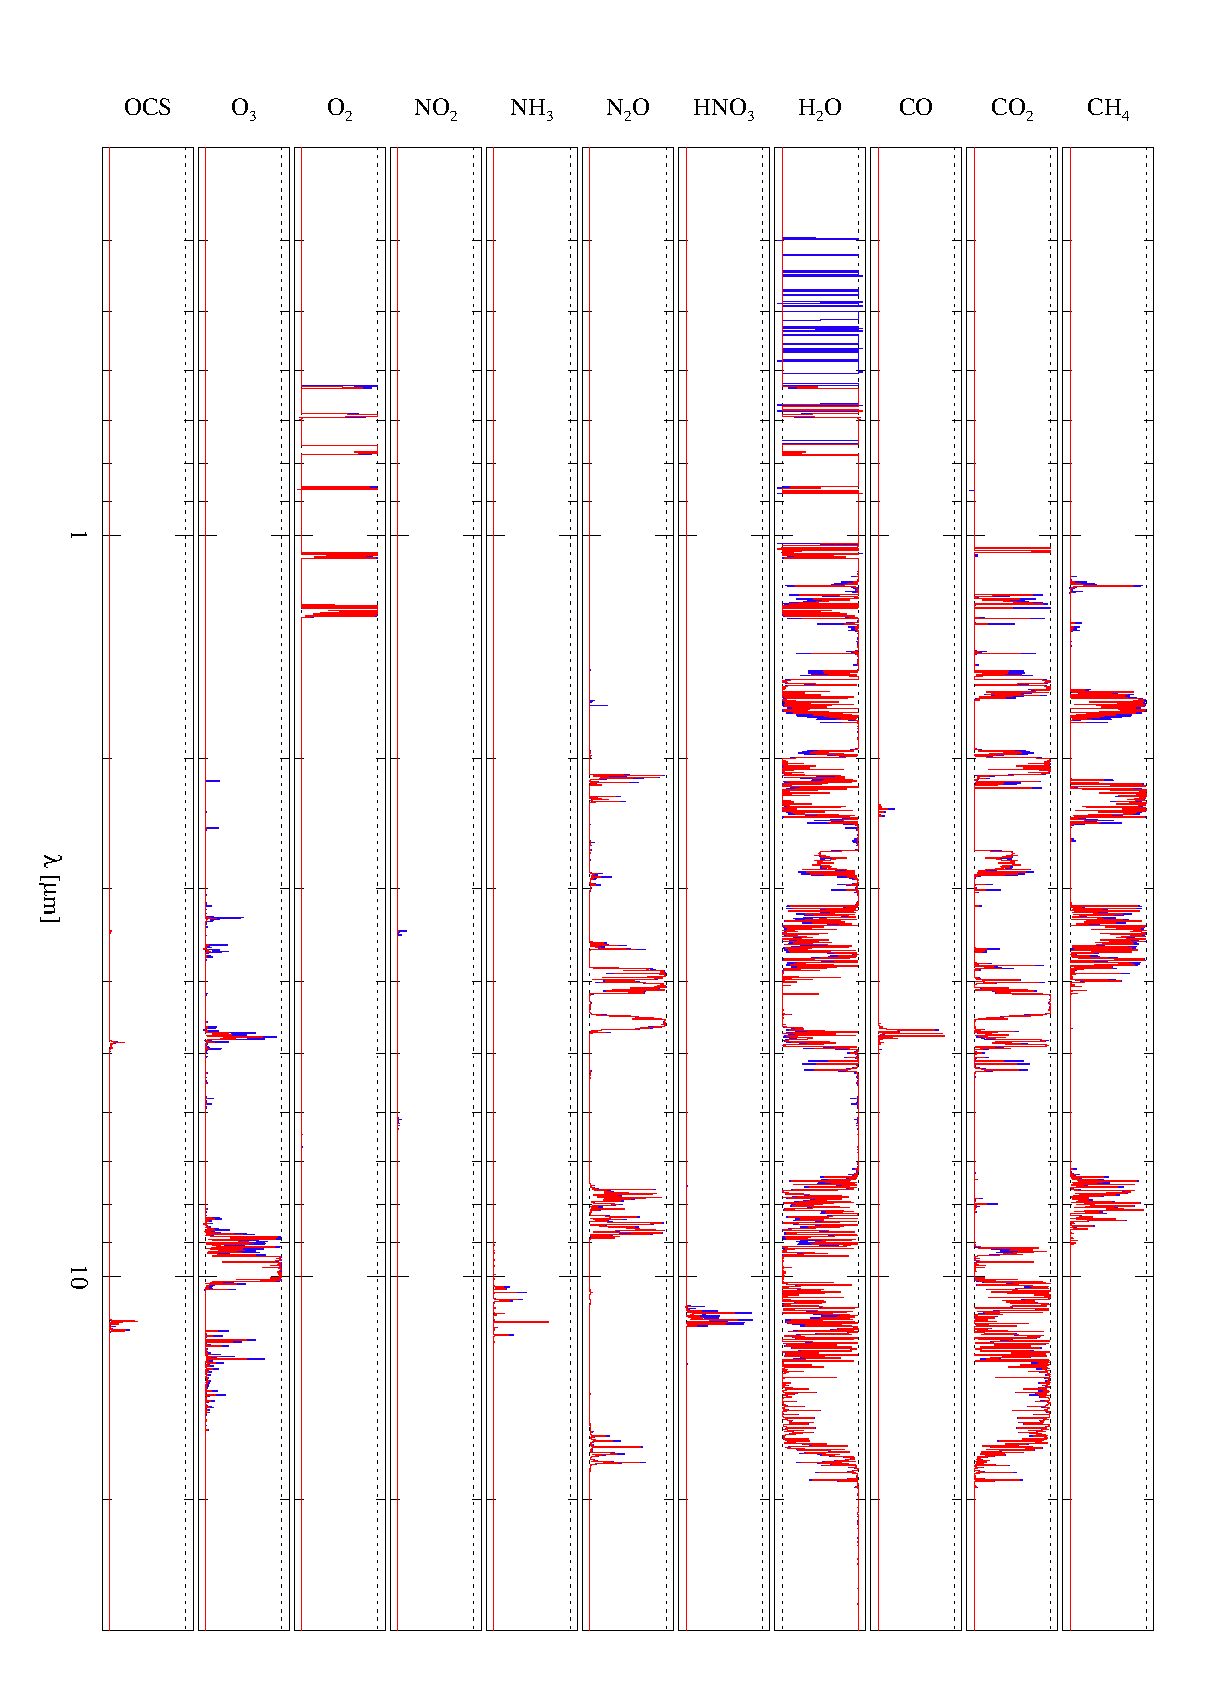
\psfig{file=figures/cheat_sheet_RT.eps,width=0.97\textwidth,angle=0}
    \caption{{\it Influence of individual molecules as a function of
    wavelength:} this figure shows the relative importance of all molecules at
    a given wavelength, which exceed more than 5\% of the total radiance (in
    red) or transmission (in blue). See text for more detail.}
    \label{fig:molecs_all}
  \end{center}
\end{figure}
%-------------------------------------------------------------------------------
\begin{figure}[ht]
  \begin{center}
    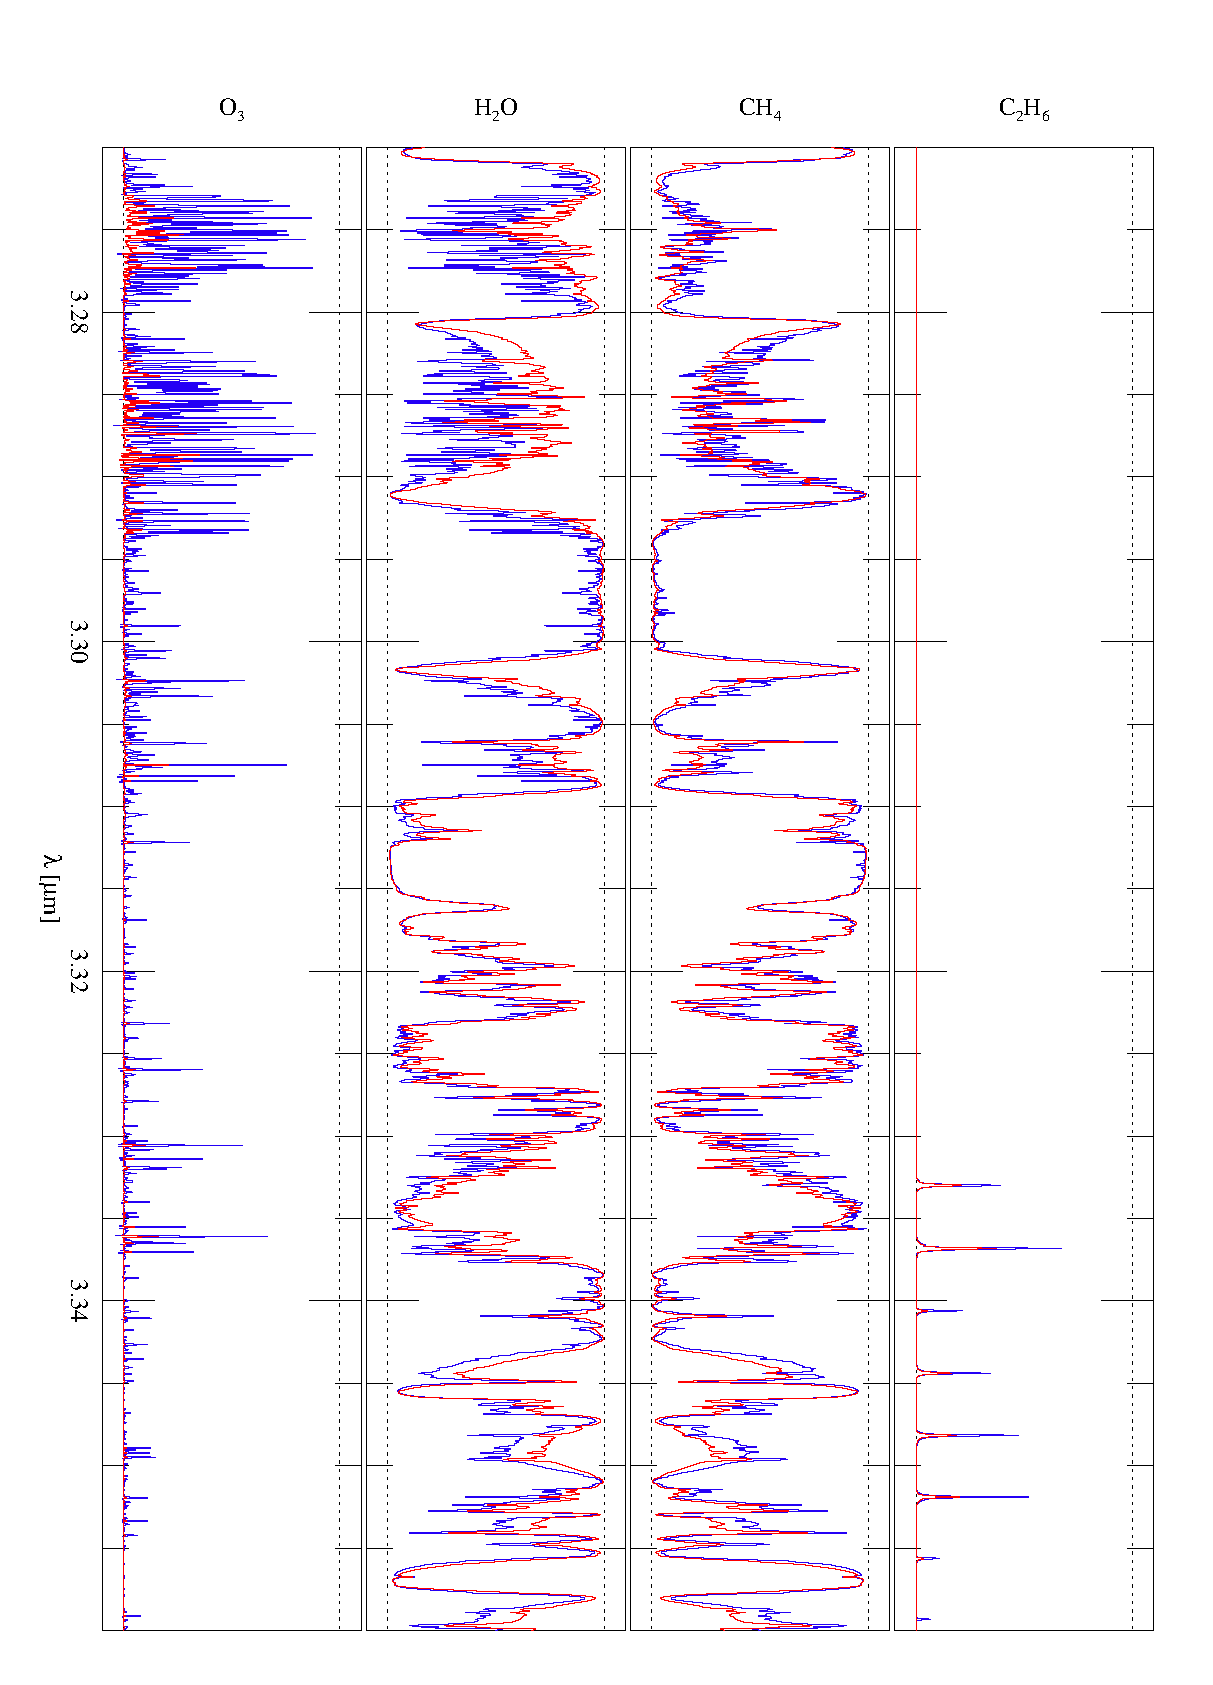
\psfig{file=figures/crires_RT.eps,width=0.97\textwidth,angle=0}
    \caption{{\it Influence of individual molecules as a function of
    wavelength:} same as Figure~\ref{fig:molecs_all}, but for the CRIRES test
    data wavelength regime. See text for more detail.}
    \label{fig:molecs_crires}
  \end{center}
\end{figure}
%-------------------------------------------------------------------------------
\begin{figure}[ht]
  \begin{center}
    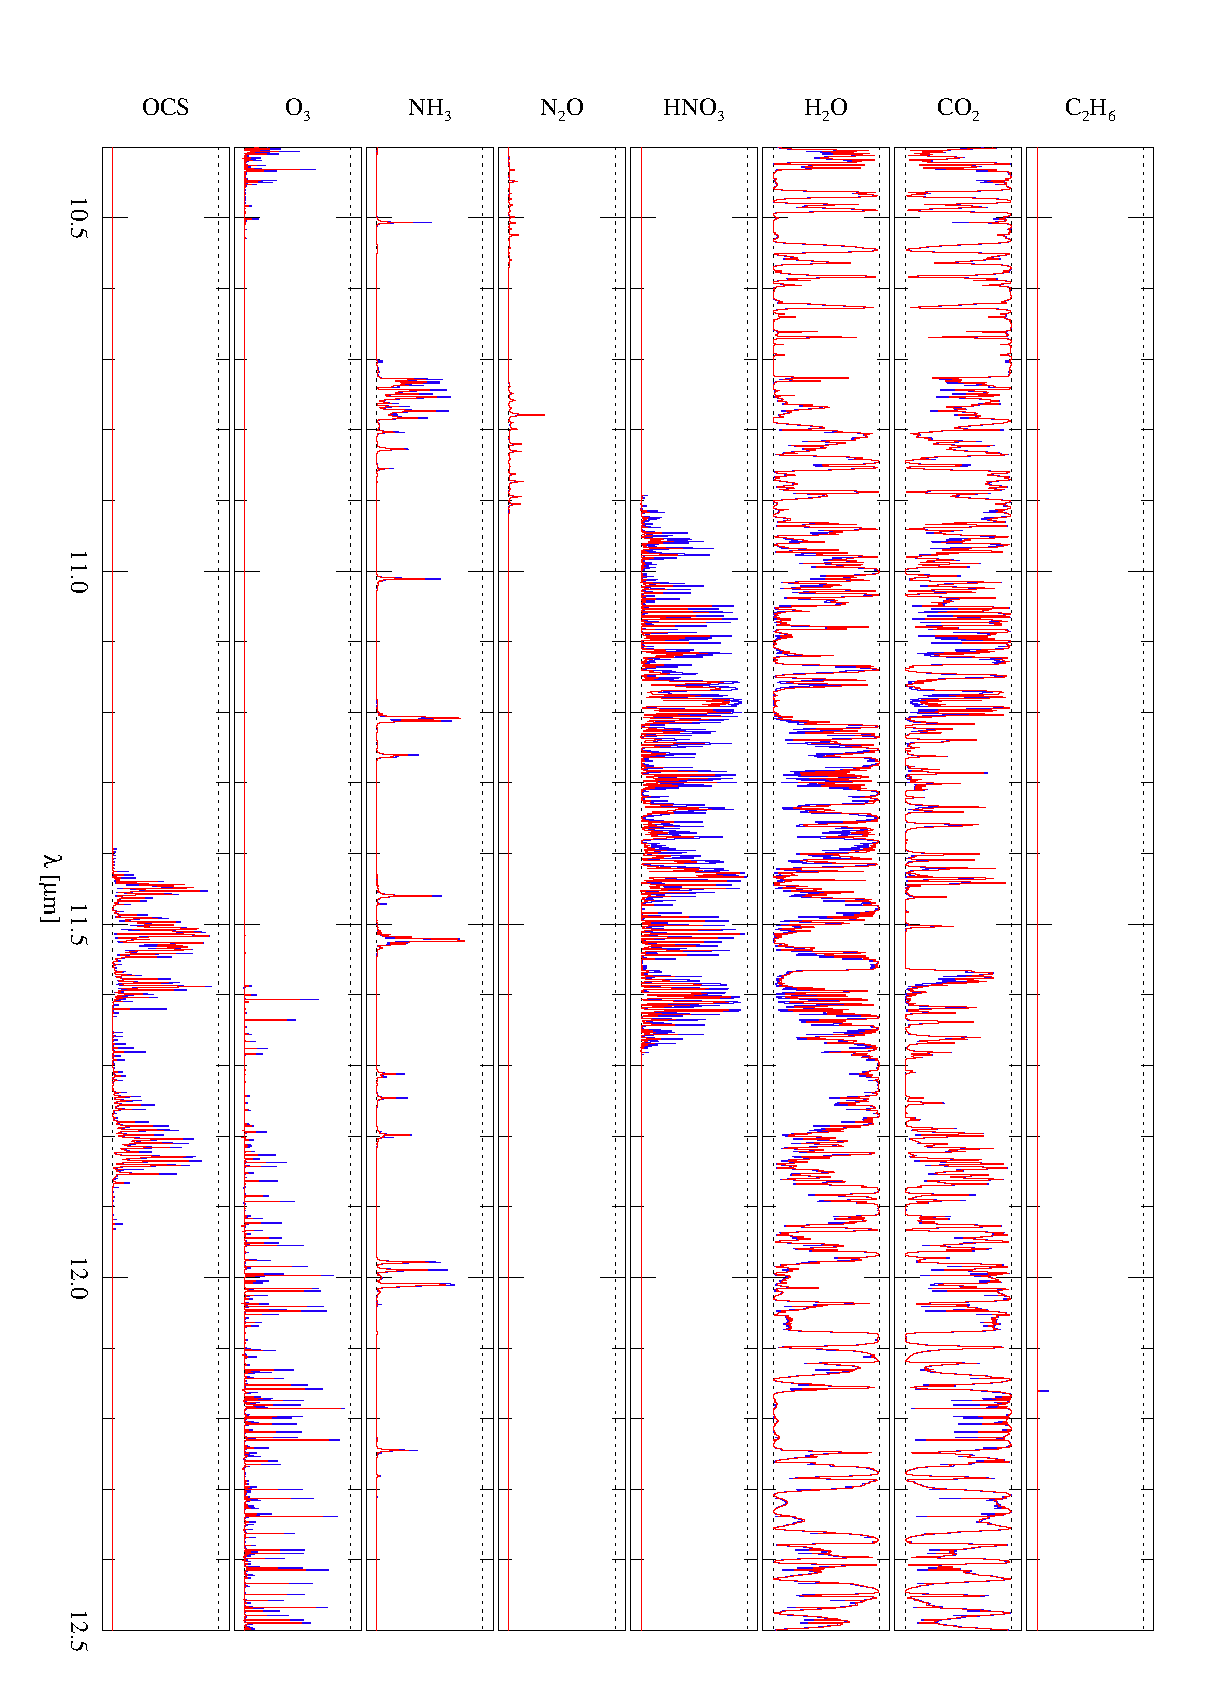
\psfig{file=figures/visir3_RT.eps,width=0.97\textwidth,angle=0}
    \caption{{\it Influence of individual molecules as a function of
    wavelength:} same as Figure~\ref{fig:molecs_all}, but for the VISIR test
    data wavelength regime. See text for more detail.}
    \label{fig:molecs_visir3}
  \end{center}
\end{figure}
%-------------------------------------------------------------------------------
\begin{figure}[ht]
    \begin{center}
    \psfig{file=figures/visir4_RT.eps,width=0.97\textwidth,angle=0}
    \caption{{\it Influence of individual molecules as a function of
    wavelength:} same as Figure~\ref{fig:molecs_all}, but for the VISIR test
    data wavelength regime. See text for more detail.}
    \label{fig:molecs_visir4}
  \end{center}
\end{figure}
%-------------------------------------------------------------------------------
\begin{figure}[ht]
  \begin{center}
    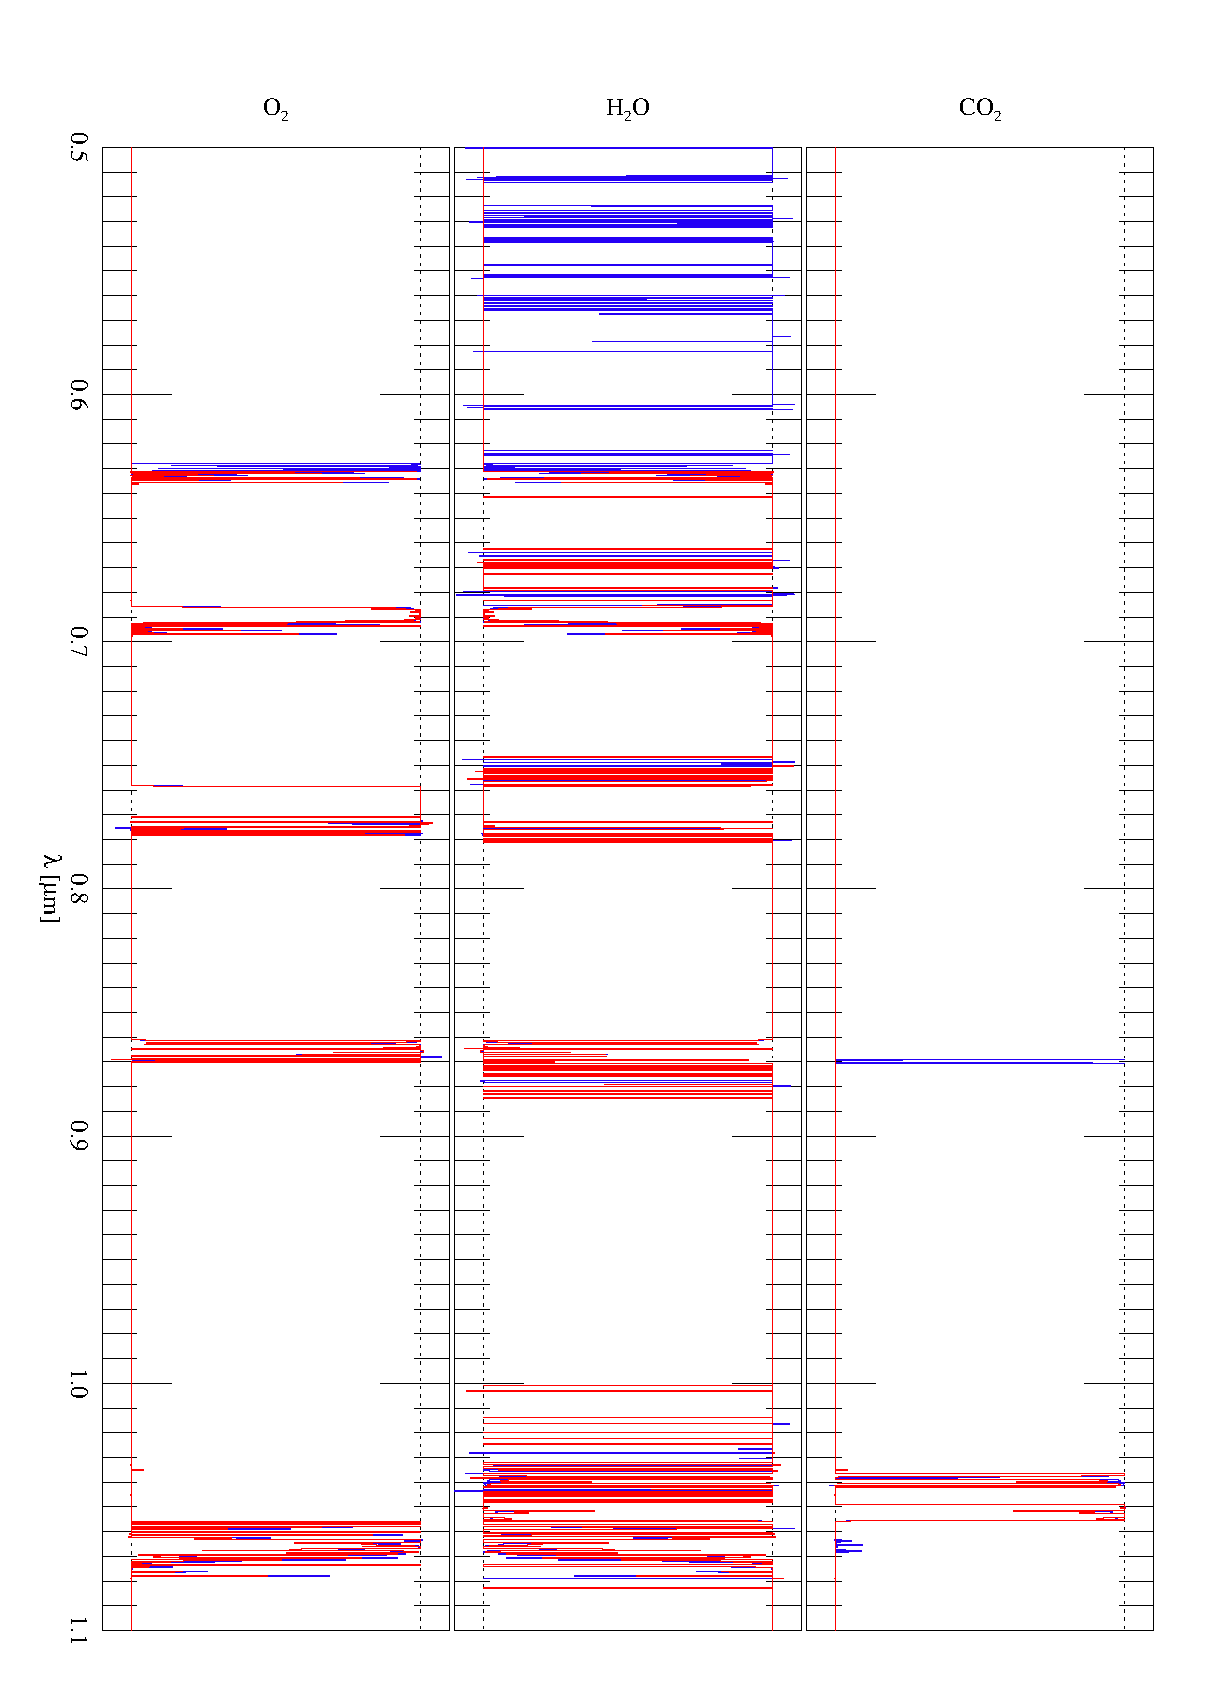
\psfig{file=figures/xshooter_RT.eps,width=0.97\textwidth,angle=0}
    \caption{{\it Influence of individual molecules as a function of
    wavelength:} same as Figure~\ref{fig:molecs_all}, but for the X-Shooter
    VIS-arm test data wavelength regime. See text for more detail.}
    \label{fig:molecs_xshoo}
  \end{center}
\end{figure}
%-------------------------------------------------------------------------------
\end{appendix}

%\clearpage

\begin{thebibliography}{99}

\section*{{\hspace{-\leftmargin}}References}

\bibitem[Anu Dudhia 2009]{anu09}
Anu Dudhia, private communication 2009

\bibitem[1992]{CLO92}
Clough, S.A., Iacono,  M.J., \& Moncet, J.-L. 1992, J. Geophys. Res., 97, 15761

\bibitem[2005]{CLO05}
Clough, S.A, Shephard, M.W., Mlawer. E.J., et al. 2005, J. Quant. Spectrosc.
Radiat. Transfer, 91, 233

\bibitem[1988]{MAS88}
Masuda, K., Takashima, T., \& Takayama, Y. 1988, Remote Sens. Environ., 24, 313

\bibitem[2010]{MOD10}
Modigliani. A., Goldoni, P., Royer, F., et al. 2010, Proc. SPIE, 7737, 773728

\bibitem[1980]{MOR80}
Mor\'e, J.J., Garbow, B.S., \& Hillstrom, K.E. 1980, User Guide for MINPACK-1,
Argonne National Laboratory Report ANL-80-74, Argonne, Ill.

\bibitem[2005]{NIR05}
Niro, F., Jucks, K., \& Hartmann, J.-M. 2005, J. Quant. Spectrosc. Radiat.
Transfer, 95, 469

\bibitem[2012]{NOL12}
Noll, S., Kausch, W., Barden, M., et al. 2012, A\&A, 543, A92

\bibitem[2011]{PAT11}
Patat, F., Moehler, S., O'Brien, K., at al. 2011, A\&A, 527, A91

\bibitem[1997]{WUS97}
Wu, X. \& Smith, L. 1997, Appl. Opt., 36, 2609 \\[0.5cm]

\bibitem[DR06-UM]{DR06UM}
DR06 User Manual, VLT-MAN-ESO-19550-5286

\bibitem[SM-01-UM]{SM01UM}
SM-01 User Manual, VLT-MAN-ESO-19550-5770

\bibitem[MF-GUI]{MFGUI}
MOLECFIT: Graphical User Interface and Tutorial, VLT-MAN-ESO-19550-5928

\bibitem[SM-03-DS]{SM03DS}
SM-03 Detailed Specification Document, VLT-SPE-ESO-19550-5769 \\[0.5cm]

\bibitem[SM-03-SR]{SM03SR}
SM-03 Science Report, VLT-TRE-ESO-19550-5774 \\[0.5cm]

\subsection*{{\hspace{-\leftmargin}}Links}

\bibitem[1]{RFM}
\texttt{http://www.atm.ox.ac.uk/RFM/}

\bibitem[2]{LBLRTM}
\texttt{http://rtweb.aer.com/lblrtm\_frame.html}

\bibitem[3]{LBLRTMFAQ}
\texttt{http://rtweb.aer.com/docs/FAQ\_LBLRTM.pdf}

\bibitem[4]{CMPFIT}
\texttt{http://www.physics.wisc.edu/~craigm/idl/cmpfit.html}

\bibitem[5]{AER}
\texttt{http://www.aer.com/}

\bibitem[6]{HITRAN}
\texttt{http://www.cfa.harvard.edu/HITRAN/}

\bibitem[7]{meteomonitor}
VLT Astronomical Site Monitor, ASM Data, User Manual, VLT-MAN-ESO-17440-1773

\bibitem[8]{NOAA}
\texttt{http://www.arl.noaa.gov/READYamet.php}

\bibitem[9]{GDAS}
\texttt{http://ready.arl.noaa.gov/gdas1.php}

\bibitem[10]{GRIB}
\texttt{http://nomads.ncep.noaa.gov/txt\_descriptions/fast\_downloading\_grib.shtml}

\bibitem[11]{GDASarchive}
\texttt{ftp://arlftp.arlhq.noaa.gov/pub/archives/gdas1/}

\bibitem[12]{LBLRTM_instructions}
\texttt{http://irina.eas.gatech.edu/Lab\_5560/lblrtm/lblrtm\_inst.html}

\bibitem[13]{Embury}
\texttt{https://www.wiki.ed.ac.uk/display/arcwiki/WP+1.1.1+Task+2}

\bibitem[14]{PWV}
\texttt{http://www.eso.org/observing/dfo/quality/GENERAL/PWV/HEALTH/}

\bibitem[15]{CDIAC}
\texttt{http://cdiac.ornl.gov/}

\bibitem[16]{CPL}
\texttt{http://www.eso.org/sci/software/cpl}

\bibitem[17]{WGRIB}
\texttt{http://www.cpc.ncep.noaa.gov/products/wesley/wgrib2}


\end{thebibliography}

\centerline{--- End of document ---}            % only if that's an even page

\end{document}
